\chapter{C++ Interface}

\section{CXCORE. Basic Functionality}

\subsection{Introduction}

Starting from OpenCV 2.0 the new modern C++ interface has been introduced.
It is crisp (less typing is needed to code the same thing), type-safe (no more CvArr $\sim$ void*)
and in general more convenient to use. Here is a short sample of what it looks like:

\begin{lstlisting}
//
// Simple retro-style photo effect done by adding noise to
// the luminance channel and reducing intensity of the chroma channels
//

// include standard OpenCV headers, same as before
#include "cv.h"
#include "highgui.h"

// all the new API is put into "cv" namespace. Export its content
using namespace cv;

// enable/disable use of mixed API in the code below.
#define DEMO_MIXED_API_USE 1

int main( int argc, char** argv )
{
    const char* imagename = argc > 1 ? argv[1] : "lena.jpg";
#if DEMO_MIXED_API_USE
    // Ptr<T> is safe ref-conting pointer class
    Ptr<IplImage> iplimg = cvLoadImage(imagename);
    
    // cv::Mat replaces the CvMat and IplImage, but it's easy to convert
    // between the old and the new data structures
    // (by default, only the header is converted and the data is shared)
    Mat img(iplimg); 
#else
    // the newer cvLoadImage alternative with MATLAB-style name
    Mat img = imread(imagename);
#endif

    if( !img.data ) // check if the image has been loaded properly
        return -1;

    Mat img_yuv;
    // convert image to YUV color space.
    // The output image will be allocated automatically
    cvtColor(img, img_yuv, CV_BGR2YCrCb); 

    // split the image into separate color planes
    vector<Mat> planes;
    split(img_yuv, planes);

    // another Mat constructor; allocates a matrix of the specified size and type
    Mat noise(img.size(), CV_8U);
    
    // fills the matrix with normally distributed random values;
    // there is also randu() for uniformly distributed random numbers. 
    // Scalar replaces CvScalar, Scalar::all() replaces cvScalarAll().
    randn(noise, Scalar::all(128), Scalar::all(20));
                                                     
    // blur the noise a bit, kernel size is 3x3 and both sigma's are set to 0.5
    GaussianBlur(noise, noise, Size(3, 3), 0.5, 0.5);

    const double brightness_gain = 0;
    const double contrast_gain = 1.7;
#if DEMO_MIXED_API_USE
    // it's easy to pass the new matrices to the functions that
    // only work with IplImage or CvMat:
    // step 1) - convert the headers, data will not be copied
    IplImage cv_planes_0 = planes[0], cv_noise = noise;
    // step 2) call the function; do not forget unary "&" to form pointers
    cvAddWeighted(&cv_planes_0, contrast_gain, &cv_noise, 1,
                 -128 + brightness_gain, &cv_planes_0);
#else
    addWeighted(planes[0], constrast_gain, noise, 1,
                -128 + brightness_gain, planes[0]);
#endif
    const double color_scale = 0.5;
    // Mat::convertTo() replaces cvConvertScale.
    // One must explicitly specify the output matrix type
    // (we keep it intact, i.e. pass planes[1].type())
    planes[1].convertTo(planes[1], planes[1].type(),
                        color_scale, 128*(1-color_scale));

    // alternative form of convertTo if we know the datatype
    // at compile time ("uchar" here).
    // This expression will not create any temporary arrays
    // and should be almost as fast as the above variant
    planes[2] = Mat_<uchar>(planes[2]*color_scale + 128*(1-color_scale));

    // Mat::mul replaces cvMul(). Again, no temporary arrays are
    // created in case of simple expressions.
    planes[0] = planes[0].mul(planes[0], 1./255);

    // now merge the results back
    merge(planes, img_yuv);
    // and produce the output RGB image
    cvtColor(img_yuv, img, CV_YCrCb2BGR);

    // this is counterpart for cvNamedWindow
    namedWindow("image with grain", CV_WINDOW_AUTOSIZE);
#if DEMO_MIXED_API_USE
    // this is to demonstrate that img and iplimg really share the data -
    // the result of the above processing is stored in img and thus in iplimg too.
    cvShowImage("image with grain", iplimg);
#else
    imshow("image with grain", img);
#endif
    waitKey();

    return 0;
    // all the memory will automatically be released
    // by vector<>, Mat and Ptr<> destructors.
}
\end{lstlisting}

In the rest of the introduction we discuss the key features of the new interface in more details.

\subsection{Namespace \texttt{cv} and Function Naming}

All the newly introduced classes and functions are placed into \texttt{cv} namespace. Therefore, to access this functionality from your code, use \texttt{cv::} specifier or \texttt{"using namespace cv;"} directive:
\begin{lstlisting}
#include "cv.h"

...
cv::Mat H = cv::findHomography(points1, points2, cv::RANSAC, 5);
...
\end{lstlisting}
or
\begin{lstlisting}
#include "cv.h"

using namespace cv;

...
Mat H = findHomography(points1, points2, RANSAC, 5 );
...
\end{lstlisting}

It is probable that some of the current or future OpenCV external names conflict with STL
or other libraries, in this case use explicit namespace specifiers to resolve the name conflicts:
\begin{lstlisting}
Mat a(100, 100, CV_32F);
randu(a, Scalar::all(1), Scalar::all(std::rand()%256+1));
cv::log(a, a);
a /= std::log(2.);
\end{lstlisting}

For most used C functions and structures from OpenCV 1.x you may find the direct counterparts in the new C++ interface. The name is usually formed by omitting \texttt{cv} or \texttt{Cv} prefix and turning the first letter to the low case (unless it's a own name, like Canny, Sobel etc). In case when there is no the new-style counterpart, it's possible to use the old functions with the new structures, as shown the first sample in the chapter.

\subsection{Memory Management}

The new interface does most of memory deallocation or even memory allocation operations automatically when needed.

First of all, \cross{Mat}, \cross{SparseMat} and other classes have destructors
that deallocate memory buffers occupied by the structures when needed.

Secondly, this "when needed" means that the destructors do not always deallocate the buffers, they take into account possible data sharing.
That is, in a destructor the reference counter associated with the underlying data is decremented and the data is deallocated
if and only if the reference counter reaches zero, that is, when no other structures use the same buffers. When such a structure
containing a reference counter is copied, usually just the header is duplicated and the underlying data is not; instead, the reference counter is incremented to memorize that there is another owner of the same data.
Also, some structures, such as \texttt{Mat}, can use pre-allocated data rather than data allocated by the structures' methods.
In this case the reference counter is \texttt{NULL} pointer and then no reference counting is done - the data is not deallocated by the destructors and should be deallocated manually by the user. We saw this scheme in the first example in the chapter:
\begin{lstlisting}
// allocates IplImages and wraps it into shared pointer class.
Ptr<IplImage> iplimg = cvLoadImage(...);

// constructs Mat header for IplImage data;
// does not copy the data;
// the reference counter will be NULL
Mat img(iplimg);
...
// in the end of the block img destructor is called,
// which does not try to deallocate the data because
// of NULL pointer to the reference counter.
//
// Then Ptr<IplImage> destructor is called that decrements
// the reference counter and if it reached 0, calls cvReleaseImage().
\end{lstlisting}

The copying semantics was mentioned in the above paragraph, but deserves a dedicated explanation.
By default, the new OpenCV structures implement cheap, so called O(1) (i.e. constant-time) assignment operations. It gives user possibility to pass quite big data structures to functions (though, \texttt{const Mat\&} is even faster), return them (e.g. see the example with \cross{findHomography} above) and store in OpenCV and STL containers, and do all of this very efficiently. On the other hand, most of the new data structures provide clone()
method that creates a full copy of an object. Here is the sample:
\begin{lstlisting}
// create a big 8Mb matrix
Mat A(1000, 1000, CV_64F);

// create another header for the same matrix;
// this is instant operation, regardless of the matrix size.
Mat B = A;
// create another header for the 3-rd row of A; no data is copied either
Mat C = B.row(3);
// now create a separate copy of the matrix
Mat D = B.clone();
// copy the 5-th row of B to C, that is, copy the 5-th row of A to the 3-rd row of A.
B.row(5).copyTo(C);
// now let A and D share the data; after that the modified version
// of A is still referenced by B and C.
A = D;
// now make B an empty matrix (which references no memory buffers),
// but the modified version of A will still be referenced by C,
// despite that C is just a single matrix row
B.release(); 
             
// finally, make a full copy of C and deallocate the modified
// big matrix, since it's not referenced by anyone
C = C.clone();
\end{lstlisting}

Memory management of the new data structures is automatic and thus easy. If, however, your code uses \cross{IplImage},
\cross{CvMat} or other C data structures a lot, memory management can still be automated without immediate migration
to \cross{Mat} by using the already mentioned template class \cross{Ptr}, similar to \texttt{shared\_ptr} from Boost and C++ TR1.
It warps a pointer to an arbitrary object, provides transparent access to all the object fields and associates a reference counter with it.
Instance of the class can be passed to any function that expects the original pointer. For correct deallocation of the object, you should specialize \texttt{Ptr<T>::delete\_obj()} method, like it was done for classic OpenCV datatypes:
\begin{lstlisting}
// cxoperations.hpp:
...
template<> inline Ptr<IplImage>::delete_obj() {
    cvReleaseImage(&obj);
}
...
\end{lstlisting}
See \cross{Ptr} description for more details and other usage scenarios.


\subsection{Memory Management Part II. Automatic Data Allocation}

With the new interface not only explicit memory deallocation is not needed anymore,
but the memory allocation is often done automatically too. That was demonstrated in the example
in the beginning of the chapter when \texttt{cvtColor} was called, and here are some more details.

\cross{Mat} and other array classes provide method \texttt{create} that allocates a new buffer for array
data if and only if the currently allocated array is not of the required size and type.
If a new buffer is needed, the previously allocated buffer is released
(by engaging all the reference counting mechanism described in the previous section).
Now, since it is very quick to check whether the needed memory buffer is already allocated,
most new OpenCV functions that have output arrays call the \texttt{create} method and
this way the Automatic Data Allocation concept is implemented. Here is the example:
\begin{lstlisting}
#include "cv.h"
#include "highgui.h"

int main(int, char**)
{
    VideoCapture cap(0);
    if(!cap.isOpened()) return -1;

    Mat edges;
    namedWindow("edges",1);
    for(;;)
    {
        Mat frame;
        cap >> frame;
        cvtColor(frame, edges, CV_BGR2GRAY);
        GaussianBlur(edges, edges, Size(7,7), 1.5, 1.5);
        Canny(edges, edges, 0, 30, 3);
        imshow("edges", edges);
        if(waitKey(30) >= 0) break;
    }
    return 0;
}
\end{lstlisting}
The matrix \texttt{edges} is allocated during the first frame processing and unless the resolution will suddenly change,
the same buffer will be reused for every next frame's edge map.

In many cases the output array type and size can be inferenced from the input arrays' respective characteristics, but not always.
In these rare cases functions take separate input parameters that specify the data type and/or size of the output arrays,
like \cross{resize}. Anyway, a vast majority of the new-style array processing functions call \texttt{create}
for each of the output array, with just a few exceptions like \texttt{mixChannels}, \texttt{RNG::fill} and some others.

Note that this output array allocation semantic is only implemented in the new functions. If you want to pass the new structures to some old OpenCV function, you should first allocate the output arrays using \texttt{create} method, then make \texttt{CvMat} or \texttt{IplImage} headers and after that call the function.

\subsection{Algebraic Operations}

Just like in v1.x, OpenCV 2.x provides basic functions operating on matrices, like \texttt{add},
\texttt{subtract}, \texttt{gemm} etc. In addition, it introduces overloaded operators that give user convenient
algebraic notation and nearly as fast as the functions. For example, here is how the least squares problem $Ax=b$
can be solved using normal equations:
\begin{lstlisting}
Mat x = (A.t()*A).inv()*(A.t()*b);
\end{lstlisting}

The complete list of overloaded operators can be found in \cross{Matrix Expressions}.

\subsection{Fast Element Access}

Historically, OpenCV provided many different ways to access image and matrix elements, and none of them was both fast and convenient.
With the new data structures, OpenCV 2.x introduces a few more alternatives, hopefully more convenient than before. For detailed description of the operations, please, check \cross{Mat} and \href{#MatT}{Mat\_} description. Here is part of the retro-photo-styling example rewritten (in simplified form) using the element access operations:

\begin{lstlisting}
...
// split the image into separate color planes
vector<Mat> planes;
split(img_yuv, planes);

// method 1. process Y plane using an iterator
MatIterator_<uchar> it = planes[0].begin<uchar>(),
                    it_end = planes[0].end<uchar>();
for(; it != it_end; ++it)
{
    double v = *it*1.7 + rand()%21-10;
    *it = saturate_cast<uchar>(v*v/255.);
}

// method 2. process the first chroma plane using pre-stored row pointer.
// method 3. process the second chroma plane using
             individual element access operations
for( int y = 0; y < img_yuv.rows; y++ )
{
    uchar* Uptr = planes[1].ptr<uchar>(y);
    for( int x = 0; x < img_yuv.cols; x++ )
    {
        Uptr[x] = saturate_cast<uchar>((Uptr[x]-128)/2 + 128);
        uchar& Vxy = planes[2].at<uchar>(y, x);
        Vxy = saturate_cast<uchar>((Vxy-128)/2 + 128);
    }
}

merge(planes, img_yuv);
...
\end{lstlisting}


\subsection{Saturation Arithmetics}

In the above sample you may have noticed \href{saturate}{saturate\_cast<>()} operator, and that's how all the pixel processing is done in OpenCV. When a result of image operation is 8-bit image with pixel values ranging from 0 to 255, each output pixel value is clipped to this available range:

\[
I(x,y)=\min(\max(value, 0), 255)
\]

and the similar rules are applied to 8-bit signed and 16-bit signed and unsigned types. This "saturation" semantics (different from usual C language "wrapping" semantics, where lowest bits are taken) is implemented in every image processing function, from the simple \texttt{cv::add} and \texttt{cvAdd} to \texttt{cv::cvtColor}, \texttt{cv::resize}, \texttt{cv::filter2D} etc.
It is not a new feature of OpenCV v2.x, it was there from very beginning. In the new version this special \href{saturate}{saturate\_cast<T>()} template operator is introduced to simplify implementation of this semantic in your own functions.


\subsection{Error handling}

The modern error handling mechanism in OpenCV uses exceptions, as opposite to the manual stack unrolling used in previous versions. When OpenCV is built in DEBUG configuration, the error handler provokes memory access violation, so that the full call stack and context can be analyzed with debugger.

\subsection{Threading and Reenterability}

OpenCV uses OpenMP to do thread some time-consuming operations. Threading can be explicitly controlled by \cross{setNumThreads} function. Also, functions and "const" methods of the classes are generally re-enterable, that is, they can be called from different threads asynchronously.

\subsection{Basic Structures}

\cvfunc{DataType}\label{DataType}
Template "traits" class for other OpenCV primitive data types

\begin{lstlisting}
template<typename _Tp> class DataType
{
    // value_type is always a synonym for _Tp.
    typedef _Tp value_type;
    
    // intermediate type used for operations on _Tp.
    // it is int for uchar, signed char, unsigned short, signed short and int,
    // float for float, double for double, ...
    typedef <...> work_type;
    // in case of multi-channel data it is the data type of each channel
    typedef <...> channel_type;
    enum
    {
        // CV_8U ... CV_64F
        depth = DataDepth<channel_type>::value,
        // 1 ... 
        channels = <...>,
        // '1u', '4i', '3f', '2d' etc.
        fmt=<...>,
        // CV_8UC3, CV_32FC2 ...
        type = CV_MAKETYPE(depth, channels)
    };
};
\end{lstlisting}

The template class \texttt{DataType} is descriptive class for OpenCV primitive data types and other types that comply with the following definition. A primitive OpenCV data type is one of \texttt{unsigned char, bool ($\sim$unsigned char), signed char, unsigned short, signed short, int, float, double} or a tuple of values of one of these types, where all the values in the tuple have the same type. If you are familiar with OpenCV \cross{CvMat}'s type notation, CV\_8U ... CV\_32FC3, CV\_64FC2 etc., when a primitive type can be defined as a type for which you can give a unique identifier in a form \verb*"CV\_<bit-depth>{U|S|F}C<number_of_channels>". A universal type able to store a single instance of such primitive data type is \cross{Vec}. Multiple instances of such a type can be stored in a \texttt{std::vector}, \texttt{Mat}, \texttt{Mat\_}, \texttt{MatND}, \texttt{MatND\_}, \texttt{SparseMat}, \texttt{SparseMat\_} or any other container that is able to store \cross{Vec} instances.
 
The class \texttt{DataType} is basically used to provide some description of any data type without adding any fields or methods to the corresponding class (and it is actually impossible to add anything to primitive C/C++ data types). This technique is known in C++ as class traits. It's not \texttt{DataType} itself that is used, but its specialized versions, such as:

\begin{lstlisting}
template<> class DataType<uchar>
{
    typedef uchar value_type;
    typedef int work_type;
    typedef uchar channel_type;
    enum { channel_type = CV_8U, channels = 1, fmt='u', type = CV_8U };
};
...
template<typename _Tp> DataType<std::complex<_Tp> >
{
    typedef std::complex<_Tp> value_type;
    typedef std::complex<_Tp> work_type;
    typedef _Tp channel_type;
    // DataDepth is another helper trait class
    enum { depth = DataDepth<_Tp>::value, channels=2,
        fmt=(channels-1)*256+DataDepth<_Tp>::fmt,
        type=CV_MAKETYPE(depth, channels) };
};
...
\end{lstlisting}

The main purpose of the classes is to convert compile time type information to OpenCV-compatible data type identifier, for example:

\begin{lstlisting}
// allocates 30x40 floating-point matrix
Mat A(30, 40, DataType<float>::type);

Mat B = Mat_<std::complex<double> >(3, 3);
// the statement below will print 6, 2 /* i.e. depth == CV_64F, channels == 2 */ 
cout << B.depth() << ", " << B.channels() << endl; 
\end{lstlisting}

that is, such traits are used to tell OpenCV which data type you are working with, even if such a type is not native. Also, this mechanism is useful for generic algorithm implementation (in particular, it is used this way internally in OpenCV).

\cvfunc{Point\_}
Template class for 2D points

\begin{lstlisting}
template<typename _Tp> class Point_
{
public:
    typedef _Tp value_type;
    
    Point_();
    Point_(_Tp _x, _Tp _y);
    Point_(const Point_& pt);
    Point_(const CvPoint& pt);
    Point_(const CvPoint2D32f& pt);
    Point_(const Size_<_Tp>& sz);
    Point_(const Vec<_Tp, 2>& v);
    Point_& operator = (const Point_& pt);
    template<typename _Tp2> operator Point_<_Tp2>() const;
    operator CvPoint() const;
    operator CvPoint2D32f() const;
    operator Vec<_Tp, 2>() const;

    // computes dot-product (this->x*pt.x + this->y*pt.y)
    _Tp dot(const Point_& pt) const;
    // computes dot-product using double-precision arithmetics
    double ddot(const Point_& pt) const;
    // returns true if the point is inside the rectangle "r".
    bool inside(const Rect_<_Tp>& r) const;
    
    _Tp x, y;
};
\end{lstlisting}

The class represents a 2D point, specified by its coordinates $x$ and $y$.
Instance of the class is interchangeable with С structures \texttt{CvPoint} and \texttt{CvPoint2D32f}. There is also cast operator to convert point coordinates to the specified type. The conversion from floating-point coordinates to integer coordinates is done by rounding; in general case the conversion uses \href{saturate}{saturate\_cast<>()} operation on each of the coordinates. Besides the class members listed in the declaration above, the following operations on points are implemented:

\begin{itemize}
    \item \texttt{pt1 = pt2 $\pm$ pt3}
    \item \texttt{pt1 = pt2 * $\alpha$, pt1 = $\alpha$ * pt2}
    \item \texttt{pt1 += pt2, pt1 -= pt2, pt1 *= $\alpha$}
    \item \texttt{double value = norm(pt); // $L_2$-norm}
    \item \texttt{pt1 == pt2, pt1 != pt2}    
\end{itemize}

For user convenience, the following type aliases are defined:
\begin{lstlisting}
typedef Point_<int> Point2i;
typedef Point2i Point;
typedef Point_<float> Point2f;
typedef Point_<double> Point2d;
\end{lstlisting}

Here is a short example:
\begin{lstlisting}
Point2f a(0.3f, 0.f), b(0.f, 0.4f);
Point pt = (a + b)*10.f;
cout << pt.x << ", " << pt.y << endl; 
\end{lstlisting}

\cvfunc{Point3\_}

Template class for 3D points

\begin{lstlisting}

template<typename _Tp> class Point3_
{
public:
    typedef _Tp value_type;
    
    Point3_();
    Point3_(_Tp _x, _Tp _y, _Tp _z);
    Point3_(const Point3_& pt);
    explicit Point3_(const Point_<_Tp>& pt);
    Point3_(const CvPoint3D32f& pt);
    Point3_(const Vec<_Tp, 3>& v);
    Point3_& operator = (const Point3_& pt);
    template<typename _Tp2> operator Point3_<_Tp2>() const;
    operator CvPoint3D32f() const;
    operator Vec<_Tp, 3>() const;

    _Tp dot(const Point3_& pt) const;
    double ddot(const Point3_& pt) const;
    
    _Tp x, y, z;
};
\end{lstlisting}

The class represents a 3D point, specified by its coordinates $x$, $y$ and $z$.
Instance of the class is interchangeable with С structure \texttt{CvPoint2D32f}. Similarly to \texttt{Point\_}, the 3D points' coordinates can be converted to another type, and the vector arithmetic and comparison operations are also supported.

The following type aliases are available:

\begin{lstlisting}
typedef Point3_<int> Point3i;
typedef Point3_<float> Point3f;
typedef Point3_<double> Point3d;
\end{lstlisting}

\cvfunc{Size\_}

Template class for specfying image or rectangle size.

\begin{lstlisting}
template<typename _Tp> class Size_
{
public:
    typedef _Tp value_type;
    
    Size_();
    Size_(_Tp _width, _Tp _height);
    Size_(const Size_& sz);
    Size_(const CvSize& sz);
    Size_(const CvSize2D32f& sz);
    Size_(const Point_<_Tp>& pt);
    Size_& operator = (const Size_& sz);
    _Tp area() const;

    operator Size_<int>() const;
    operator Size_<float>() const;
    operator Size_<double>() const;
    operator CvSize() const;
    operator CvSize2D32f() const;

    _Tp width, height;
};
\end{lstlisting}

The class \texttt{Size\_} is similar to \texttt{Point\_}, except that the two members are called \texttt{width} and \texttt{height} instead of \texttt{x} and \texttt{y}. The structure can be converted to and from the old OpenCV structures \cross{CvSize} and \cross{CvSize2D32f}. The same set of arithmetic and comparison operations as for \texttt{Point\_} is available. 

OpenCV defines the following type aliases:

\begin{lstlisting}
typedef Size_<int> Size2i;
typedef Size2i Size;
typedef Size_<float> Size2f;
\end{lstlisting}

\cvfunc{Rect\_}

Template class for 2D rectangles

\begin{lstlisting}
template<typename _Tp> class Rect_
{
public:
    typedef _Tp value_type;
    
    Rect_();
    Rect_(_Tp _x, _Tp _y, _Tp _width, _Tp _height);
    Rect_(const Rect_& r);
    Rect_(const CvRect& r);
    // (x, y) <- org, (width, height) <- sz
    Rect_(const Point_<_Tp>& org, const Size_<_Tp>& sz);
    // (x, y) <- min(pt1, pt2), (width, height) <- max(pt1, pt2) - (x, y)
    Rect_(const Point_<_Tp>& pt1, const Point_<_Tp>& pt2);
    Rect_& operator = ( const Rect_& r );
    // returns Point_<_Tp>(x, y)
    Point_<_Tp> tl() const;
    // returns Point_<_Tp>(x+width, y+height)
    Point_<_Tp> br() const;
    
    // returns Size_<_Tp>(width, height)
    Size_<_Tp> size() const;
    // returns width*height
    _Tp area() const;

    operator Rect_<int>() const;
    operator Rect_<float>() const;
    operator Rect_<double>() const;
    operator CvRect() const;

    // x <= pt.x && pt.x < x + width &&
    // y <= pt.y && pt.y < y + height ? true : false
    bool contains(const Point_<_Tp>& pt) const;

    _Tp x, y, width, height;
};
\end{lstlisting}

The rectangle is described by the coordinates of the top-left corner (which is the default interpretation of \texttt{Rect\_::x} and \texttt{Rect\_::y} in OpenCV; though, in your algorithms you may treat \texttt{x} and \texttt{y} as coordinates of the bottom-left corner), the rectangle width and height. Another assumption OpenCV usually makes is that the top and left boundary of the rectangle are inclusive, while the right and bottom boundaries are not, for example, the method \texttt{Rect\_::contains} returns true if
\begin{eqnarray*}
      x \leq pt.x < x+width,\\
      y \leq pt.y < y+height
\end{eqnarray*}
And virtually every loop over an image \cross{ROI} in OpenCV (where ROI is specified by \texttt{Rect\_<int>}) is implemented as:
\begin{lstlisting}
for(int y = roi.y; y < roi.y + rect.height; y++)
    for(int x = roi.x; x < roi.x + rect.width; x++)
    {
        // ...
    }
\end{lstlisting}

In addition to the class members, the following operations on rectangles are implemented:
\begin{itemize}
    \item \texttt{rect1 = rect1 $\pm$ point1} (shifting rectangle by a certain offset)
    \item \texttt{rect1 = rect1 $\pm$ size1} (expanding or shrinking rectangle by a certain amount)
    \item \texttt{rect1 += point1, rect1 -= point1, rect1 += size1, rect1 -= size1} (augmenting operations)
    \item \texttt{rect1 = rect2 \& rect3} (rectangle intersection)
    \item \texttt{rect1 = rect2 | rect3} (minimum area rectangle containing \texttt{rect2} and \texttt{rect3})
    \item \texttt{rect1 \&= rect2, rect1 |= rect2} (and the corresponding augmenting operations)
    \item \texttt{rect1 == rect2, rect1 != rect2} (rectangle comparison)
\end{itemize}

Example. Here is how the partial ordering on rectangles can be established (rect1 $\subseteq$ rect2):
\begin{lstlisting}
template<typename _Tp> inline bool
operator <= (const Rect_<_Tp>& r1, const Rect_<_Tp>& r2)
{
    return (r1 & r2) == r1;
}
\end{lstlisting}

For user convenience, the following type alias is available:
\begin{lstlisting}
typedef Rect_<int> Rect;
\end{lstlisting}

\cvfunc{RotatedRect}\label{RotatedRect}
Possibly rotated rectangle

\begin{lstlisting}
class RotatedRect
{
public:
    // constructors
    RotatedRect();
    RotatedRect(const Point2f& _center, const Size2f& _size, float _angle);
    RotatedRect(const CvBox2D& box);
    
    // returns minimal up-right rectangle that contains the rotated rectangle
    Rect boundingRect() const;
    // backward conversion to CvBox2D
    operator CvBox2D() const;
    
    // mass center of the rectangle
    Point2f center;
    // size
    Size2f size;
    // rotation angle in degrees
    float angle;
};
\end{lstlisting}

The class \texttt{RotatedRect} replaces the old \cross{CvBox2D} and fully compatible with it.

\cvfunc{TermCriteria}\label{TermCriteria}

Termination criteria for iterative algorithms

\begin{lstlisting}
class TermCriteria
{
public:
    enum { COUNT=1, MAX_ITER=COUNT, EPS=2 };

    // constructors
    TermCriteria();
    // type can be MAX_ITER, EPS or MAX_ITER+EPS.
    // type = MAX_ITER means that only the number of iterations does matter;
    // type = EPS means that only the required precision (epsilon) does matter
    //    (though, most algorithms put some limit on the number of iterations anyway)
    // type = MAX_ITER + EPS means that algorithm stops when
    // either the specified number of iterations is made,
    // or when the specified accuracy is achieved - whatever happens first.
    TermCriteria(int _type, int _maxCount, double _epsilon);
    TermCriteria(const CvTermCriteria& criteria);
    operator CvTermCriteria() const;

    int type;
    int maxCount;
    double epsilon;
};
\end{lstlisting}

The class \texttt{TermCriteria} replaces the old \cross{CvTermCriteria} and fully compatible with it.


\cvfunc{Vec}\label{Vec}
Template class for short numerical vectors

\begin{lstlisting}
template<typename _Tp, int cn> class Vec
{
public:
    typedef _Tp value_type;
    enum { depth = DataDepth<_Tp>::value, channels = cn,
           type = CV_MAKETYPE(depth, channels) };
    
    // default constructor: all elements are set to 0
    Vec();
    // constructors taking up to 10 first elements as parameters
    Vec(_Tp v0);
    Vec(_Tp v0, _Tp v1);
    Vec(_Tp v0, _Tp v1, _Tp v2);
    ...
    Vec(_Tp v0, _Tp v1, _Tp v2, _Tp v3, _Tp v4,
        _Tp v5, _Tp v6, _Tp v7, _Tp v8, _Tp v9);
    Vec(const Vec<_Tp, cn>& v);
    // constructs vector with all the components set to alpha.
    static Vec all(_Tp alpha);
    
    // two variants of dot-product
    _Tp dot(const Vec& v) const;
    double ddot(const Vec& v) const;
    
    // cross-product; valid only when cn == 3.
    Vec cross(const Vec& v) const;
    
    // element type conversion
    template<typename T2> operator Vec<T2, cn>() const;
    
    // conversion to/from CvScalar (valid only when cn==4)
    operator CvScalar() const;
    
    // element access
    _Tp operator [](int i) const;
    _Tp& operator[](int i);

    _Tp val[cn];
};
\end{lstlisting}

The class is most universal representation of short numerical vectors or tuples. It is possible to convert \texttt{Vec<T,2>} to/from \texttt{Point\_}, \texttt{Vec<T,3>} to/from \texttt{Point3\_} and \texttt{Vec<T,4>} to \cross{CvScalar}. The elements of \texttt{Vec} are accessed using \texttt{operator[]} and expected vector operations are implemented too:

\begin{itemize}
    \item \texttt{v1 = v2 $\pm$ v3, v1 = v2 * $\alpha$, v1 = $\alpha * v2$} (plus the corresponding augmenting operations; note that these operations apply \href{saturate}{saturate\_cast<\_Tp>()} to the each computed vector component)
    \item \texttt{v1 == v2, v1 != v2}
    \item \texttt{double n = norm(v1); // $L_2$-norm}
\end{itemize}

For user convenience, the following type aliases are introduced:
\begin{lstlisting}
typedef Vec<uchar, 2> Vec2b;
typedef Vec<uchar, 3> Vec3b;
typedef Vec<uchar, 4> Vec4b;

typedef Vec<short, 2> Vec2s;
typedef Vec<short, 3> Vec3s;
typedef Vec<short, 4> Vec4s;

typedef Vec<int, 2> Vec2i;
typedef Vec<int, 3> Vec3i;
typedef Vec<int, 4> Vec4i;

typedef Vec<float, 2> Vec2f;
typedef Vec<float, 3> Vec3f;
typedef Vec<float, 4> Vec4f;
typedef Vec<float, 6> Vec6f;

typedef Vec<double, 2> Vec2d;
typedef Vec<double, 3> Vec3d;
typedef Vec<double, 4> Vec4d;
typedef Vec<double, 6> Vec6d;
\end{lstlisting}

The class \texttt{Vec} can be used for declaring various numerical objects, e.g. \texttt{Vec<double,9>} can be used to store a 3x3 double-precision matrix. It is also very useful for declaring and processing multi-channel arrays, see \texttt{Mat\_} description.

\cvfunc{Scalar\_}
4-element vector

\begin{lstlisting}
template<typename _Tp> class Scalar_ : public Vec<_Tp, 4>
{
public:
    Scalar_();
    Scalar_(_Tp v0, _Tp v1, _Tp v2=0, _Tp v3=0);
    Scalar_(const CvScalar& s);
    Scalar_(_Tp v0);
    static Scalar_<_Tp> all(_Tp v0);
    operator CvScalar() const;

    template<typename T2> operator Scalar_<T2>() const;

    Scalar_<_Tp> mul(const Scalar_<_Tp>& t, double scale=1 ) const;
    template<typename T2> void convertTo(T2* buf, int channels, int unroll_to=0) const;
};

typedef Scalar_<double> Scalar;
\end{lstlisting}

The template class \texttt{Scalar\_} and it's double-precision instantiation \texttt{Scalar} represent 4-element vector. They are absolutely similar to \texttt{Vec<\_Tp, 4>} expect that they can be constructed from \texttt{CvScalar}. \texttt{Scalar} is widely used in OpenCV for passing pixel values and it is a drop-in replacement for \cross{CvScalar} that was used for the same purpose in the earlier versions of OpenCV.

\cvfunc{Range}\label{Range}
Specifies a continuous subsequence (a.k.a. slice) of a sequence.

\begin{lstlisting}
class Range
{
public:
    Range();
    Range(int _start, int _end);
    Range(const CvSlice& slice);
    int size() const;
    bool empty() const;
    static Range all();
    operator CvSlice() const;

    int start, end;
};
\end{lstlisting}

The class is used to specify a row or column span in a matrix (\cross{Mat}), and for many other purposes. \texttt{Range(a,b)} is basically the same as \texttt{a:b} in Matlab or \texttt{a..b} in Python. As in Python, \texttt{start} is inclusive left boundary of the range, and \texttt{end} is exclusive right boundary of the range. Such a half-opened interval is usually denoted as $[start,end)$.

The static method \texttt{Range::all()} returns some special variable that means "the whole sequence" or "the whole range", just like "\texttt{:}" in Matlab or "\texttt{...}" in Python. All the methods and functions in OpenCV that take \texttt{Range} support this special \texttt{Range::all()} value, but of course, in case of your own custom processing you will probably have to implement it manually:
\begin{lstlisting}
void my_function(..., const Range& r, ....)
{
    if(r == Range::all()) {
        // process all the data
    }
    else {
        // process [r.start, r.end)
    } 
}
\end{lstlisting}

\cvfunc{Mat}\label{Mat}

OpenCV C++ matrix class.

\begin{lstlisting}
class Mat
{
public:
    // constructors
    Mat();
    // constructs matrix of the specified size and type
    // (_type is CV_8UC1, CV_64FC3, CV_32SC(12) etc.)
    Mat(int _rows, int _cols, int _type);
    // constucts matrix and fills it with the specified value _s.
    Mat(int _rows, int _cols, int _type, const Scalar& _s);
    Mat(Size _size, int _type);
    // copy constructor
    Mat(const Mat& m);
    // constructor for matrix headers pointing to user-allocated data
    Mat(int _rows, int _cols, int _type, void* _data, size_t _step=AUTO_STEP);
    Mat(Size _size, int _type, void* _data, size_t _step=AUTO_STEP);
    // creates a matrix header for a part of the bigger matrix
    Mat(const Mat& m, const Range& rowRange, const Range& colRange);
    Mat(const Mat& m, const Rect& roi);
    // converts old-style CvMat to the new matrix; the data is not copied by default
    Mat(const CvMat* m, bool copyData=false);
    // converts old-style IplImage to the new matrix; the data is not copied by default
    Mat(const IplImage* img, bool copyData=false);
    // builds matrix from std::vector with or without copying the data
    template<typename _Tp> Mat(const vector<_Tp>& vec, bool copyData=false);
    // helper constructor to compile matrix expressions
    Mat(const MatExpr_Base& expr);
    // destructor - calls release()
    ~Mat();
    // assignment operators
    Mat& operator = (const Mat& m);
    Mat& operator = (const MatExpr_Base& expr);

    ...
    // returns a new matrix header for the specified row
    Mat row(int y) const;
    // returns a new matrix header for the specified column
    Mat col(int x) const;
    // ... for the specified row span
    Mat rowRange(int startrow, int endrow) const;
    Mat rowRange(const Range& r) const;
    // ... for the specified column span
    Mat colRange(int startcol, int endcol) const;
    Mat colRange(const Range& r) const;
    // ... for the specified diagonal
    // (d=0 - the main diagonal,
    //  >0 - a diagonal from the lower half,
    //  <0 - a diagonal from the upper half)
    Mat diag(int d=0) const;
    // constructs a square diagonal matrix which main diagonal is vector "d"
    static Mat diag(const Mat& d);

    // returns deep copy of the matrix, i.e. the data is copied
    Mat clone() const;
    // copies the matrix content to "m".
    // It calls m.create(this->size(), this->type()).
    void copyTo( Mat& m ) const;
    // copies those matrix elements to "m" that are marked with non-zero mask elements.
    void copyTo( Mat& m, const Mat& mask ) const;
    // converts matrix to another datatype with optional scalng. See cvConvertScale.
    void convertTo( Mat& m, int rtype, double alpha=1, double beta=0 ) const;

    ...
    // sets every matrix element to s
    Mat& operator = (const Scalar& s);
    // sets some of the matrix elements to s, according to the mask
    Mat& setTo(const Scalar& s, const Mat& mask=Mat());
    // creates alternative matrix header for the same data, with different
    // number of channels and/or different number of rows. see cvReshape.
    Mat reshape(int _cn, int _rows=0) const;

    // matrix transposition by means of matrix expressions
    MatExpr_<...> t() const;
    // matrix inversion by means of matrix expressions
    MatExpr_<...> inv(int method=DECOMP_LU) const;
    // per-element matrix multiplication by means of matrix expressions
    MatExpr_<...> mul(const Mat& m, double scale=1) const;
    MatExpr_<...> mul(const MatExpr_<...>& m, double scale=1) const;

    // computes cross-product of 2 3D vectors
    Mat cross(const Mat& m) const;
    // computes dot-product
    double dot(const Mat& m) const;

    // Matlab-style matrix initialization. see the description
    static MatExpr_Initializer zeros(int rows, int cols, int type);
    static MatExpr_Initializer zeros(Size size, int type);
    static MatExpr_Initializer ones(int rows, int cols, int type);
    static MatExpr_Initializer ones(Size size, int type);
    static MatExpr_Initializer eye(int rows, int cols, int type);
    static MatExpr_Initializer eye(Size size, int type);
    
    // allocates new matrix data unless the matrix already has specified size and type.
    // previous data is unreferenced if needed.
    void create(int _rows, int _cols, int _type);
    void create(Size _size, int _type);
    // increases the reference counter; use with care to avoid memleaks
    void addref();
    // decreases reference counter;
    // deallocate the data when reference counter reaches 0.
    void release();

    // locates matrix header within a parent matrix. See below
    void locateROI( Size& wholeSize, Point& ofs ) const;
    // moves/resizes the current matrix ROI inside the parent matrix.
    Mat& adjustROI( int dtop, int dbottom, int dleft, int dright );
    // extracts a rectangular sub-matrix
    // (this is a generalized form of row, rowRange etc.)
    Mat operator()( Range rowRange, Range colRange ) const;
    Mat operator()( const Rect& roi ) const;

    // converts header to CvMat; no data is copied
    operator CvMat() const;
    // converts header to IplImage; no data is copied
    operator IplImage() const;
    
    // returns true iff the matrix data is continuous
    // (i.e. when there are no gaps between successive rows).
    // similar to CV_IS_MAT_CONT(cvmat->type)
    bool isContinuous() const;
    // returns element size in bytes,
    // similar to CV_ELEM_SIZE(cvmat->type)
    size_t elemSize() const;
    // returns the size of element channel in bytes.
    size_t elemSize1() const;
    // returns element type, similar to CV_MAT_TYPE(cvmat->type)
    int type() const;
    // returns element type, similar to CV_MAT_DEPTH(cvmat->type)
    int depth() const;
    // returns element type, similar to CV_MAT_CN(cvmat->type)
    int channels() const;
    // returns step/elemSize1()
    size_t step1() const;
    // returns matrix size:
    // width == number of columns, height == number of rows
    Size size() const;
    // returns true if matrix data is NULL
    bool empty() const;

    // returns pointer to y-th row
    uchar* ptr(int y=0);
    const uchar* ptr(int y=0) const;

    // template version of the above method
    template<typename _Tp> _Tp* ptr(int y=0);
    template<typename _Tp> const _Tp* ptr(int y=0) const;
    
    // template methods for read-write or read-only element access.
    // note that _Tp must match the actual matrix type -
    // the functions do not do any on-fly type conversion
    template<typename _Tp> _Tp& at(int y, int x);
    template<typename _Tp> _Tp& at(Point pt);
    template<typename _Tp> const _Tp& at(int y, int x) const;
    template<typename _Tp> const _Tp& at(Point pt) const;
    
    // template methods for iteration over matrix elements.
    // the iterators take care of skipping gaps in the end of rows (if any)
    template<typename _Tp> MatIterator_<_Tp> begin();
    template<typename _Tp> MatIterator_<_Tp> end();
    template<typename _Tp> MatConstIterator_<_Tp> begin() const;
    template<typename _Tp> MatConstIterator_<_Tp> end() const;

    enum { MAGIC_VAL=0x42FF0000, AUTO_STEP=0, CONTINUOUS_FLAG=CV_MAT_CONT_FLAG };

    // includes several bit-fields:
    //  * the magic signature
    //  * continuity flag
    //  * depth
    //  * number of channels
    int flags;
    // the number of rows and columns
    int rows, cols;
    // a distance between successive rows in bytes; includes the gap if any
    size_t step;
    // pointer to the data
    uchar* data;

    // pointer to the reference counter;
    // when matrix points to user-allocated data, the pointer is NULL
    int* refcount;
    
    // helper fields used in locateROI and adjustROI
    uchar* datastart;
    uchar* dataend;
};
\end{lstlisting}

The class \texttt{Mat} represents a 2D numerical array that can act as a matrix (and further it's referred to as a matrix), image, optical flow map etc. It is very similar to \cross{CvMat} type from earlier versions of OpenCV, and similarly to \texttt{CvMat}, the matrix can be multi-channel, but it also fully supports \cross{ROI} mechanism, just like \cross{IplImage}.

There are many different ways to create \texttt{Mat} object. Here are the some popular ones:
\begin{itemize}
\item using \texttt{create(nrows, ncols, type)} method or
    similar \texttt{Mat(nrows, ncols, type[, fill\_value])} constructor.
    A new matrix of the specified size and specifed type is allocated.
    \texttt{type} has the same meaning as in \cross{cvCreateMat} method,
    e.g. \texttt{CV\_8UC1} means 8-bit single-channel matrix,
    \texttt{CV\_32FC2} means 2-channel (i.e. complex) floating-point matrix etc:
        
\begin{lstlisting}
// make 7x7 complex matrix filled with 1+3j.
cv::Mat M(7,7,CV_32FC2,Scalar(1,3));
// and now turn M to 100x60 15-channel 8-bit matrix.
// The old content will be deallocated
M.create(100,60,CV_8UC(15));
\end{lstlisting}
        
    As noted in the introduction of this chapter, \texttt{create()}
    will only allocate a new matrix when the current matrix dimensionality
    or type is different from the specified.
        
\item by using a copy constructor or assignment operator, where on the right side it can
      be a matrix or expression, see below. Again, as noted in the introduction,
      matrix assignment is O(1) operation because it only copies the header
      and increases the reference counter. \texttt{Mat::clone()} method can be used to get full
      (a.k.a. deep) copy of the matrix when you need it.
          
\item by constructing a header for a part of another matrix. It can be a single row, single column,
      several rows, several columns, rectangular region in the matrix (called a minor in algebra) or
      a diagonal. Such operation is also O(1) operation because the new header will reference the same data.
      You can actually modify a part of the matrix using this feature, e.g.
          
\begin{lstlisting}
// add 5-th row, multiplied by 3 to the 3rd row
M.row(3) = M.row(3) + M.row(5)*3;

// create new 320x240 image
cv::Mat img(Size(320,240),CV_8UC3);
// select a roi
cv::Mat roi(img, Rect(10,10,100,100));
// fill the ROI with (0,255,0) (which is green in RGB space);
// the original 320x240 image will be modified
roi = Scalar(0,255,0);
\end{lstlisting}

      Thanks to the additional \texttt{datastart} and \texttt{dataend} members, it is possible to
      compute the relative sub-matrix position in the main \emph{"container"} matrix using \texttt{locateROI()}:
      
\begin{lstlisting}
Mat A = Mat::eye(10, 10, CV_32S);
// extracts A columns, 1 (inclusive) to 3 (exclusive).
Mat B = A(Range::all(), Range(1, 3));
// extracts B rows, 5 (inclusive) to 9 (exclusive).
// that is, C ~ A(Range(5, 9), Range(1, 3))
Mat C = B(Range(5, 9), Range::all());
Size size; Point ofs;
C.locateROI(size, ofs);
// size will be (10,10) and ofs will be (/*x=*/1, /*y=*/5)
\end{lstlisting}
          
      As in case of whole matrices, if you need a deep copy, use \texttt{clone()} method
      of the extracted sub-matrices.
          
\item by making a header for user-allocated-data. It can be useful for
    \begin{enumerate}
        \item processing "foreign" data using OpenCV (e.g. when you implement
        DirectShow filter or gstreamer processing module), e.g.
            
\begin{lstlisting}
void process_video_frame(const unsigned char* pixels,
                         int width, int height, int step)
{
    cv::Mat img(height, width, CV_8UC3, pixels, step);
    cv::GaussianBlur(img, img, Size(7,7), 1.5, 1.5);
}
\end{lstlisting}
            
        \item for quick initialization of small matrices and/or super-fast element access
\begin{lstlisting}
double m[3][3] = {{a, b, c}, {d, e, f}, {g, h, i}};
cv::Mat M(3, 3, CV_64F, m);
M = M.inv();
\end{lstlisting}
        \end{enumerate}
        
        partial yet very common cases of this "user-allocated data" case are conversions
        from \cross{CvMat} and \cross{IplImage} to \texttt{Mat}. For this purpose there are special constructors
        taking pointers to \texttt{CvMat} or \texttt{IplImage} and the optional
        flag indicating whether to copy the data or not.
        
        Backward conversion from \texttt{Mat} to \texttt{CvMat} or \texttt{IplImage} is provided via cast operators
        \texttt{Mat::operator CvMat() const} an \texttt{Mat::operator IplImage()}.
        The operators do \emph{not} copy the data.
        
\item by using MATLAB-style matrix initializers, \texttt{zeros(), ones(), eye()}, e.g.:

\begin{lstlisting}
// create 100x100 double-precision identity martix and add it to M.
M += Mat::eye(100, 100, CV_64F);
\end{lstlisting}

\item by using comma-separated initializer:
\begin{lstlisting}
// create 3x3 double-precision identity matrix
Mat M = (Mat_<double>(3,3) << 1, 0, 0, 0, 1, 0, 0, 0, 1);
\end{lstlisting}

here we first call constructor of \texttt{Mat\_} class (that we describe further) with the proper matrix, and then we just put << operator followed by comma-separated values that can be constants, variables, expressions etc. Also, note the extra parentheses that are needed to avoid compiler errors.
        
\end{itemize}

Once matrix is created, it will be automatically managed by using reference-counting mechanism (unless the matrix header is built on top of user-allocated data, in which case you should handle the data yourself).
So the matrix data will be deallocated when no one points to it; if you want to release the data pointed by a matrix header before the matrix destructor is called, the \texttt{Mat::release()} method is the safe way to do it.

The next important thing to learn about matrix is element access. Here is how the matrix is stored. The elements are stored in row-major order (row by row). The \texttt{data} member points to the first element of the first row, \texttt{rows} contains the number of matrix rows and \texttt{cols} -- the number of matrix columns. There is yet another member, called \texttt{step} that is used to actually compute address of a matrix element. The \texttt{step} is needed because the matrix can be a part of another matrix or because there can some padding space for proper alignment in the end of each row:
%\includegraphics[width=1.0\textwidth]{pics/roi.png}
Given these parameters, address of the matrix element $M_{ij}$ is computed as following:


\texttt{addr($M_{ij}$)=M.data + M.step*i + j*M.elemSize()}


if you know matrix element type, e.g. it is \texttt{float}, then you can use \texttt{at<>()} method:


\texttt{addr($M_{ij}$)=\&M.at<float>(i,j)}

(where \& is used to convert the reference returned by \texttt{at} to a pointer).
if you need to process a whole row of matrix, much more efficient way is to get the pointer to the row first, and then just use plain C operator []:

\begin{lstlisting}
// compute sum of positive matrix elements
// (assuming that M is double-precision matrix)
double sum=0;
for(int i = 0; i < M.rows; i++)
{
    const double* Mi = M.ptr<double>(i);
    for(int j = 0; j < M.cols; j++)
        sum += std::max(Mi[j], 0.);
}
\end{lstlisting}

Some operations, like the above one, do not actually depend on the matrix shape, they just process elements of a matrix one by one (or elements from multiple matrices that are sitting in the same place, e.g. matrix addition). Such operations are called element-wise and it makes sense to check whether all the input/output matrices are continuous, i.e. have no gaps in the end of each row, and if yes, process them as a single long row:

\begin{lstlisting}
// compute sum of positive matrix elements, optimized variant
double sum=0;
int cols = M.cols, rows = M.rows;
if(M.isContinuous())
{
    cols *= rows;
    rows = 1;
}
for(int i = 0; i < rows; i++)
{
    const double* Mi = M.ptr<double>(i);
    for(int j = 0; j < cols; j++)
        sum += std::max(Mi[j], 0.);
}
\end{lstlisting}
In case of continuous matrix the loop body will be executed only once, so the overhead will be smaller, which will be especially noticeable in case of small matrices.

Finally, there are STL-style iterators that are smart enough to skip gaps between successive rows:
\begin{lstlisting}
// compute sum of positive matrix elements, iterator-based variant
double sum=0;
MatConstIterator_<double> it = M.begin<double>(), it_end = M.end<double>();
for(; it != it_end; ++it)
    sum += std::max(*it, 0.);
\end{lstlisting}

The matrix iterators are random-access iterators, so they can be passed to arbitrary STL algorithm, including \texttt{std::sort()}.

\cvfunc{Matrix Expressions}

This is a list of implemented matrix operations that can be combined in arbitrary complex expressions
(here \emph{A}, \emph{B} stand for matrices (\texttt{Mat}), \emph{s} for a scalar (\texttt{Scalar}),
\emph{$\alpha$} for a real-valued scalar (\texttt{double})):

\begin{itemize}
    \item addition, subtraction, negation: \texttt{A$\pm$ B, A$\pm$ s, s$\pm$ A, -A}
    \item scaling: \texttt{A*$\alpha$, A/$\alpha$}
    \item per-element multiplication and division: \texttt{A.mul(B), A/B, $\alpha$/A}
    \item matrix multiplication: \texttt{A*B}
    \item transposition: \texttt{A.t() $\sim A^t$}
    \item matrix inversion and pseudo-inversion, solving linear systems and least-squares problems:
        \texttt{A.inv([method]) $\sim A^{-1}$}, \texttt{A.inv([method])*B $\sim X:\,AX=B$}
    \item comparison: \texttt{A$\gtreqqless$ B, A $\ne$ B, A$\gtreqqless \alpha$, A $\ne \alpha$}
          (the result of comparison is 8-bit single channel mask, which elements are set to 255
          (if the particular element or pair of elements satisfy the condition) and 0 otherwise)
    \item bitwise logical operations: \verb"A & B, A & s, A | B, A | s, A ^ B, A ^ s, ~A"
    \item element-wise minimum and maximum: \texttt{min(A, B), min(A, $\alpha$), max(A, B), max(A, $\alpha$)}
    \item element-wise absolute value: \texttt{abs(A)}
    \item cross-product, dot-product: \texttt{A.cross(B), A.dot(B)}
    \item any function of matrix or matrices and scalars that returns a matrix or a scalar, such as
          \cross{norm}, \cross{mean}, \cross{sum}, \cross{countNonZero}, \cross{trace},
          \cross{determinant}, \cross{repeat} etc.
    \item matrix initializers (\texttt{eye(), zeros(), ones()}), matrix comma-separated initializers,
          matrix constructors and operators that extract sub-matrices (see \cross{Mat} description).
    \item \verb"Mat_<destination_type>()" constructors to cast the result to the proper type.
\end{itemize}
Note, however, that comma-separated initializers and probably some other operations may require additional explicit \texttt{Mat()} or \verb"Mat_<T>()" constuctor calls to resolve possible ambiguity.

\cvfunc{Mat\_}
Template matrix class derived from \cross{Mat}

\begin{lstlisting}
template<typename _Tp> class Mat_ : public Mat
{
public:
    typedef _Tp value_type;
    typedef typename DataType<_Tp>::channel_type channel_type;
    typedef MatIterator_<_Tp> iterator;
    typedef MatConstIterator_<_Tp> const_iterator;

    Mat_();
    // equivalent to Mat(_rows, _cols, DataType<_Tp>::type)
    Mat_(int _rows, int _cols);
    // other forms of the above constructor
    Mat_(int _rows, int _cols, const _Tp& value);
    explicit Mat_(Size _size);
    Mat_(Size _size, const _Tp& value);
    // copy/conversion contructor. If m is of different type, it's converted
    Mat_(const Mat& m);
    // copy constructor
    Mat_(const Mat_& m);
    // construct a matrix on top of user-allocated data.
    // step is in bytes(!!!), regardless of the type
    Mat_(int _rows, int _cols, _Tp* _data, size_t _step=AUTO_STEP);
    // minor selection
    Mat_(const Mat_& m, const Range& rowRange, const Range& colRange);
    Mat_(const Mat_& m, const Rect& roi);
    // to support complex matrix expressions
    Mat_(const MatExpr_Base& expr);
    // makes a matrix out of Vec or std::vector. The matrix will have a single column
    template<int n> explicit Mat_(const Vec<_Tp, n>& vec);
    Mat_(const vector<_Tp>& vec, bool copyData=false);

    Mat_& operator = (const Mat& m);
    Mat_& operator = (const Mat_& m);
    // set all the elements to s.
    Mat_& operator = (const _Tp& s);

    // iterators; they are smart enough to skip gaps in the end of rows
    iterator begin();
    iterator end();
    const_iterator begin() const;
    const_iterator end() const;

    // equivalent to Mat::create(_rows, _cols, DataType<_Tp>::type)
    void create(int _rows, int _cols);
    void create(Size _size);
    // cross-product
    Mat_ cross(const Mat_& m) const;
    // to support complex matrix expressions
    Mat_& operator = (const MatExpr_Base& expr);
    // data type conversion
    template<typename T2> operator Mat_<T2>() const;
    // overridden forms of Mat::row() etc.
    Mat_ row(int y) const;
    Mat_ col(int x) const;
    Mat_ diag(int d=0) const;
    Mat_ clone() const;

    // transposition, inversion, per-element multiplication
    MatExpr_<...> t() const;
    MatExpr_<...> inv(int method=DECOMP_LU) const;

    MatExpr_<...> mul(const Mat_& m, double scale=1) const;
    MatExpr_<...> mul(const MatExpr_<...>& m, double scale=1) const;

    // overridden forms of Mat::elemSize() etc.
    size_t elemSize() const;
    size_t elemSize1() const;
    int type() const;
    int depth() const;
    int channels() const;
    size_t step1() const;
    // returns step()/sizeof(_Tp)
    size_t stepT() const;

    // overridden forms of Mat::zeros() etc. Data type is omitted, of course
    static MatExpr_Initializer zeros(int rows, int cols);
    static MatExpr_Initializer zeros(Size size);
    static MatExpr_Initializer ones(int rows, int cols);
    static MatExpr_Initializer ones(Size size);
    static MatExpr_Initializer eye(int rows, int cols);
    static MatExpr_Initializer eye(Size size);

    // some more overriden methods
    Mat_ reshape(int _rows) const;
    Mat_& adjustROI( int dtop, int dbottom, int dleft, int dright );
    Mat_ operator()( const Range& rowRange, const Range& colRange ) const;
    Mat_ operator()( const Rect& roi ) const;

    // more convenient forms of row and element access operators 
    _Tp* operator [](int y);
    const _Tp* operator [](int y) const;

    _Tp& operator ()(int row, int col);
    const _Tp& operator ()(int row, int col) const;
    _Tp& operator ()(Point pt);
    const _Tp& operator ()(Point pt) const;

    // to support matrix expressions
    operator MatExpr_<Mat_, Mat_>() const;
    
    // conversion to vector.
    operator vector<_Tp>() const;
};
\end{lstlisting}

The class \texttt{Mat\_<\_Tp>} is a "thin" template wrapper on top of \texttt{Mat} class. It does not have any extra data fields, nor it or \texttt{Mat} have any virtual methods and thus references or pointers to these two classes can be freely converted one to another. But do it with care, e.g.:

\begin{lstlisting}
// create 100x100 8-bit matrix
Mat M(100,100,CV_8U);
// this will compile fine. no any data conversion will be done.
Mat_<float>& M1 = (Mat_<float>&)M;
// the program will likely at the statement below
M1(99,99) = 1.f;
\end{lstlisting}

While \texttt{Mat} is sufficient in most cases, \texttt{Mat\_} can be more convenient if you use a lot of element access operations and if you know matrix type at compile time. Note that \texttt{Mat::at<\_Tp>(int y, int x)} and \texttt{Mat\_<\_Tp>::operator ()(int y, int x)} do absolutely the same and run at the same speed, but the latter is certainly shorter:

\begin{lstlisting}
Mat_<double> M(20,20);
for(int i = 0; i < M.rows; i++)
    for(int j = 0; j < M.cols; j++)
        M(i,j) = 1./(i+j+1);
Mat E, V;
eigen(M,E,V);
cout << E.at<double>(0,0)/E.at<double>(M.rows-1,0);
\end{lstlisting}

\emph{How to use \texttt{Mat\_} for multi-channel images/matrices?}

This is simple - just pass \texttt{Vec} as \texttt{Mat\_} parameter:
\begin{lstlisting}
// allocate 320x240 color image and fill it with green (in RGB space)
Mat_<Vec3b> img(240, 320, Vec3b(0,255,0));
// now draw a diagonal white line
for(int i = 0; i < 100; i++)
    img(i,i)=Vec3b(255,255,255);
// and now scramble the 2nd (red) channel of each pixel
for(int i = 0; i < img.rows; i++)
    for(int j = 0; j < img.cols; j++)
        img(i,j)[2] ^= (uchar)(i ^ j);
\end{lstlisting}

\cvfunc{MatND}\label{MatND}
n-dimensional dense array

\begin{lstlisting}
class MatND
{
public:
    // default constructor
    MatND();
    // constructs array with specific size and data type
    MatND(int _ndims, const int* _sizes, int _type);
    // constructs array and fills it with the specified value
    MatND(int _ndims, const int* _sizes, int _type, const Scalar& _s);
    // copy constructor. only the header is copied.
    MatND(const MatND& m);
    // sub-array selection. only the header is copied
    MatND(const MatND& m, const Range* ranges);
    // converts old-style nd array to MatND; optionally, copies the data
    MatND(const CvMatND* m, bool copyData=false);
    ~MatND();
    MatND& operator = (const MatND& m);

    // creates a complete copy of the matrix (all the data is copied)
    MatND clone() const;
    // sub-array selection; only the header is copied
    MatND operator()(const Range* ranges) const;

    // copies the data to another matrix.
    // Calls m.create(this->size(), this->type()) prior to
    // copying the data
    void copyTo( MatND& m ) const;
    // copies only the selected elements to another matrix.
    void copyTo( MatND& m, const MatND& mask ) const;
    // converts data to the specified data type.
    // calls m.create(this->size(), rtype) prior to the conversion
    void convertTo( MatND& m, int rtype, double alpha=1, double beta=0 ) const;

    // assigns "s" to each array element. 
    MatND& operator = (const Scalar& s);
    // assigns "s" to the selected elements of array
    // (or to all the elements if mask==MatND())
    MatND& setTo(const Scalar& s, const MatND& mask=MatND());
    // modifies geometry of array without copying the data
    MatND reshape(int _newcn, int _newndims=0, const int* _newsz=0) const;

    // allocates a new buffer for the data unless the current one already
    // has the specified size and type.
    void create(int _ndims, const int* _sizes, int _type);
    // manually increment reference counter (use with care !!!)
    void addref();
    // decrements the reference counter. Dealloctes the data when
    // the reference counter reaches zero.
    void release();

    // converts the matrix to 2D Mat or to the old-style CvMatND.
    // In either case the data is not copied.
    operator Mat() const;
    operator CvMatND() const;
    // returns true if the array data is stored continuously 
    bool isContinuous() const;
    // returns size of each element in bytes
    size_t elemSize() const;
    // returns size of each element channel in bytes
    size_t elemSize1() const;
    // returns OpenCV data type id (CV_8UC1, ... CV_64FC4,...)
    int type() const;
    // returns depth (CV_8U ... CV_64F)
    int depth() const;
    // returns the number of channels
    int channels() const;
    // step1() ~ step()/elemSize1()
    size_t step1(int i) const;

    // return pointer to the element (versions for 1D, 2D, 3D and generic nD cases)
    uchar* ptr(int i0);
    const uchar* ptr(int i0) const;
    uchar* ptr(int i0, int i1);
    const uchar* ptr(int i0, int i1) const;
    uchar* ptr(int i0, int i1, int i2);
    const uchar* ptr(int i0, int i1, int i2) const;
    uchar* ptr(const int* idx);
    const uchar* ptr(const int* idx) const;

    // convenient template methods for element access.
    // note that _Tp must match the actual matrix type -
    // the functions do not do any on-fly type conversion
    template<typename _Tp> _Tp& at(int i0);
    template<typename _Tp> const _Tp& at(int i0) const;
    template<typename _Tp> _Tp& at(int i0, int i1);
    template<typename _Tp> const _Tp& at(int i0, int i1) const;
    template<typename _Tp> _Tp& at(int i0, int i1, int i2);
    template<typename _Tp> const _Tp& at(int i0, int i1, int i2) const;
    template<typename _Tp> _Tp& at(const int* idx);
    template<typename _Tp> const _Tp& at(const int* idx) const;

    enum { MAGIC_VAL=0x42FE0000, AUTO_STEP=-1,
        CONTINUOUS_FLAG=CV_MAT_CONT_FLAG, MAX_DIM=CV_MAX_DIM };

    // combines data type, continuity flag, signature (magic value) 
    int flags;
    // the array dimensionality
    int dims;

    // data reference counter
    int* refcount;
    // pointer to the data
    uchar* data;
    // and its actual beginning and end
    uchar* datastart;
    uchar* dataend;

    // step and size for each dimension, MAX_DIM at max
    int size[MAX_DIM];
    size_t step[MAX_DIM];
};
\end{lstlisting}

The class \texttt{MatND} describes n-dimensional dense numerical single-channel or multi-channel array. This is a convenient representation for multi-dimensional histograms (when they are not very sparse, otherwise \texttt{SparseMat} will do better), voxel volumes, stacked motion fields etc. The data layout of matrix $M$ is defined by the array of \texttt{M.step[i]}, so that the address of element $(i_0,...,i_{M.dims-1})$, where $0\leq i_k<M.size[k]$ is computed as:
\[
addr(M_{i_0,...,i_{M.dims-1}}) = M.data + M.step[0]*i_0 + M.step[1]*i_1 + ... + M.step[M.dims-1]*i_{M.dims-1}
\]
which is more general form of the respective formula for \cross{Mat}, wherein \texttt{size[0]}$\sim$\texttt{rows},
\texttt{size[1]}$\sim$\texttt{cols}, \texttt{step[0]} was simply called \texttt{step}, and \texttt{step[1]} was not stored at all but computed as \texttt{Mat::elemSize()}.

In other aspects \texttt{MatND} is also very similar to \texttt{Mat}, with the following limitations and differences:
\begin{itemize}
    \item much less operations are implemented for \texttt{MatND}
    \item currently, algebraic expressions with \texttt{MatND} are not supported
    \item the \texttt{MatND} iterator is completely different from \texttt{Mat} and \texttt{Mat\_} iterators. The latter are per-element iterators, while the former is per-slice iterator, see below.
\end{itemize}

Here is how you can use \texttt{MatND} to compute NxNxN histogram of color 8bpp image (i.e. each channel value ranges from 0..255 and we quantize it to 0..N-1):

\begin{lstlisting}
void computeColorHist(const Mat& image, MatND& hist, int N)
{
    const int histSize[] = {N, N, N};
    
    // make sure that the histogram has proper size and type
    hist.create(3, histSize, CV_32F);
    
    // and clear it
    hist = Scalar(0);
    
    // the loop below assumes that we the image
    // is 8-bit 3-channel, so let's check it.
    CV_Assert(image.type() == CV_8UC3);
    MatConstIterator_<Vec3b> it = image.begin<Vec3b>(),
                             it_end = image.end<Vec3b>();    
    for( ; it != it_end; ++it )
    {
        const Vec3b& pix = *it;
        
        // we could have added 1.f/(image.rows*image.cols)
        // instead of 1.f to make the histogram normalized.
        hist.at<float>(pix[0]*N/256, pix[1]*N/256, pix[2]*N/256) += 1.f;
    }
}
\end{lstlisting}

And here is how you can iterate through \texttt{MatND} elements:

\begin{lstlisting}
void normalizeColorHist(MatND& hist)
{
#if 1    
    // intialize iterator (the style is different from STL).
    // after initialization the iterator will contain
    // the number of slices or planes
    // the iterator will go through
    MatNDIterator it(hist);
    double s = 0;
    // iterate through the matrix. on each iteration
    // it.planes[*] (of type Mat) will be set to the current plane.
    for(int p = 0; p < it.nplanes; p++, ++it)
        s += sum(it.planes[0])[0];
    it = MatNDIterator(hist);
    s = 1./s;
    for(int p = 0; p < it.nplanes; p++, ++it)
        it.planes[0] *= s;
#elif 1
    // this is a shorter implementation of the above
    // using built-in operations on MatND
    double s = sum(hist)[0];
    hist.convertTo(hist, hist.type(), 1./s, 0);
#else
    // and this is even shorter one
    // (assuming that the histogram elements are non-negative)
    normalize(hist, hist, 1, 0, NORM_L1);
#endif
}
\end{lstlisting}

You can iterate though several matrices simultaneously as long as they have the same geometry (dimensionality and all the dimension sizes are the same), which is useful for binary and n-ary operations on such matrices. Just pass those matrices to \texttt{MatNDIterator}. Then, during the iteration \texttt{it.planes[0]}, \texttt{it.planes[1]}, ... will be the slices of the corresponding matrices.

\cvfunc{MatND\_}
Template class for n-dimensional dense array derived from \cross{MatND}.

\begin{lstlisting}
template<typename _Tp> class MatND_ : public MatND
{
public:
    typedef _Tp value_type;
    typedef typename DataType<_Tp>::channel_type channel_type;

    // constructors, the same as in MatND, only the type is omitted
    MatND_();
    MatND_(int dims, const int* _sizes);
    MatND_(int dims, const int* _sizes, const _Tp& _s);
    MatND_(const MatND& m);
    MatND_(const MatND_& m);
    MatND_(const MatND_& m, const Range* ranges);
    MatND_(const CvMatND* m, bool copyData=false);
    MatND_& operator = (const MatND& m);
    MatND_& operator = (const MatND_& m);
    // different initialization function
    // where we take _Tp instead of Scalar
    MatND_& operator = (const _Tp& s);

    // no special destructor is needed; use the one from MatND

    void create(int dims, const int* _sizes);
    template<typename T2> operator MatND_<T2>() const;
    MatND_ clone() const;
    MatND_ operator()(const Range* ranges) const;

    size_t elemSize() const;
    size_t elemSize1() const;
    int type() const;
    int depth() const;
    int channels() const;
    // step[i]/elemSize()
    size_t stepT(int i) const;
    size_t step1(int i) const;

    // shorter alternatives for MatND::at<_Tp>.
    _Tp& operator ()(const int* idx);
    const _Tp& operator ()(const int* idx) const;
    _Tp& operator ()(int idx0);
    const _Tp& operator ()(int idx0) const;
    _Tp& operator ()(int idx0, int idx1);
    const _Tp& operator ()(int idx0, int idx1) const;
    _Tp& operator ()(int idx0, int idx1, int idx2);
    const _Tp& operator ()(int idx0, int idx1, int idx2) const;
    _Tp& operator ()(int idx0, int idx1, int idx2);
    const _Tp& operator ()(int idx0, int idx1, int idx2) const;
};
\end{lstlisting}

\texttt{MatND\_} relates to \texttt{MatND}  almost like \texttt{Mat\_} to \texttt{Mat} - it provides a bit more convenient element access operations and adds no extra members of virtual methods to the base class, thus references/pointers to \texttt{MatND\_} and \texttt{MatND} can be easily converted one to another, e.g.

\begin{lstlisting}
// alternative variant of the above histogram accumulation loop
...
CV_Assert(hist.type() == CV_32FC1);
MatND_<float>& _hist = (MatND_<float>&)hist;
for( ; it != it_end; ++it )
{
    const Vec3b& pix = *it;
    _hist(pix[0]*N/256, pix[1]*N/256, pix[2]*N/256) += 1.f;
}
...
\end{lstlisting}

\cvfunc{SparseMat}\label{SparseMat}
Sparse n-dimensional array.

\begin{lstlisting}
class SparseMat
{
public:
    typedef SparseMatIterator iterator;
    typedef SparseMatConstIterator const_iterator;

    // internal structure - sparse matrix header
    struct Hdr
    {
        ...
    };

    // sparse matrix node - element of a hash table
    struct Node
    {
        size_t hashval;
        size_t next;
        int idx[CV_MAX_DIM];
    };

    ////////// constructors and destructor //////////
    // default constructor
    SparseMat();
    // creates matrix of the specified size and type
    SparseMat(int dims, const int* _sizes, int _type);
    // copy constructor
    SparseMat(const SparseMat& m);
    // converts dense 2d matrix to the sparse form,
    // if try1d is true and matrix is a single-column matrix (Nx1),
    // then the sparse matrix will be 1-dimensional.
    SparseMat(const Mat& m, bool try1d=false);
    // converts dense n-d matrix to the sparse form
    SparseMat(const MatND& m);
    // converts old-style sparse matrix to the new-style.
    // all the data is copied, so that "m" can be safely
    // deleted after the conversion
    SparseMat(const CvSparseMat* m);
    // destructor
    ~SparseMat();
    
    ///////// assignment operations /////////// 
    
    // this is O(1) operation; no data is copied
    SparseMat& operator = (const SparseMat& m);
    // (equivalent to the corresponding constructor with try1d=false)
    SparseMat& operator = (const Mat& m);
    SparseMat& operator = (const MatND& m);

    // creates full copy of the matrix
    SparseMat clone() const;
    
    // copy all the data to the destination matrix.
    // the destination will be reallocated if needed.
    void copyTo( SparseMat& m ) const;
    // converts 1D or 2D sparse matrix to dense 2D matrix.
    // If the sparse matrix is 1D, then the result will
    // be a single-column matrix.
    void copyTo( Mat& m ) const;
    // converts arbitrary sparse matrix to dense matrix.
    // watch out the memory!
    void copyTo( MatND& m ) const;
    // multiplies all the matrix elements by the specified scalar
    void convertTo( SparseMat& m, int rtype, double alpha=1 ) const;
    // converts sparse matrix to dense matrix with optional type conversion and scaling.
    // When rtype=-1, the destination element type will be the same
    // as the sparse matrix element type.
    // Otherwise rtype will specify the depth and
    // the number of channels will remain the same is in the sparse matrix
    void convertTo( Mat& m, int rtype, double alpha=1, double beta=0 ) const;
    void convertTo( MatND& m, int rtype, double alpha=1, double beta=0 ) const;

    // not used now
    void assignTo( SparseMat& m, int type=-1 ) const;

    // reallocates sparse matrix. If it was already of the proper size and type,
    // it is simply cleared with clear(), otherwise,
    // the old matrix is released (using release()) and the new one is allocated.
    void create(int dims, const int* _sizes, int _type);
    // sets all the matrix elements to 0, which means clearing the hash table.
    void clear();
    // manually increases reference counter to the header.
    void addref();
    // decreses the header reference counter, when it reaches 0,
    // the header and all the underlying data are deallocated.
    void release();

    // converts sparse matrix to the old-style representation.
    // all the elements are copied.
    operator CvSparseMat*() const;
    // size of each element in bytes
    // (the matrix nodes will be bigger because of
    //  element indices and other SparseMat::Node elements).
    size_t elemSize() const;
    // elemSize()/channels()
    size_t elemSize1() const;
    
    // the same is in Mat and MatND
    int type() const;
    int depth() const;
    int channels() const;
    
    // returns the array of sizes and 0 if the matrix is not allocated
    const int* size() const;
    // returns i-th size (or 0)
    int size(int i) const;
    // returns the matrix dimensionality
    int dims() const;
    // returns the number of non-zero elements
    size_t nzcount() const;
    
    // compute element hash value from the element indices:
    // 1D case
    size_t hash(int i0) const;
    // 2D case
    size_t hash(int i0, int i1) const;
    // 3D case
    size_t hash(int i0, int i1, int i2) const;
    // n-D case
    size_t hash(const int* idx) const;
    
    // low-level element-acccess functions,
    // special variants for 1D, 2D, 3D cases and the generic one for n-D case.
    //
    // return pointer to the matrix element.
    //  if the element is there (it's non-zero), the pointer to it is returned
    //  if it's not there and createMissing=false, NULL pointer is returned
    //  if it's not there and createMissing=true, then the new element
    //    is created and initialized with 0. Pointer to it is returned
    //  If the optional hashval pointer is not NULL, the element hash value is
    //  not computed, but *hashval is taken instead.
    uchar* ptr(int i0, bool createMissing, size_t* hashval=0);
    uchar* ptr(int i0, int i1, bool createMissing, size_t* hashval=0);
    uchar* ptr(int i0, int i1, int i2, bool createMissing, size_t* hashval=0);
    uchar* ptr(const int* idx, bool createMissing, size_t* hashval=0);

    // higher-level element access functions:
    // ref<_Tp>(i0,...[,hashval]) - equivalent to *(_Tp*)ptr(i0,...true[,hashval]).
    //    always return valid reference to the element.
    //    If it's did not exist, it is created.
    // find<_Tp>(i0,...[,hashval]) - equivalent to (_const Tp*)ptr(i0,...false[,hashval]).
    //    return pointer to the element or NULL pointer if the element is not there.
    // value<_Tp>(i0,...[,hashval]) - equivalent to
    //    { const _Tp* p = find<_Tp>(i0,...[,hashval]); return p ? *p : _Tp(); }
    //    that is, 0 is returned when the element is not there.
    // note that _Tp must match the actual matrix type -
    // the functions do not do any on-fly type conversion
    
    // 1D case
    template<typename _Tp> _Tp& ref(int i0, size_t* hashval=0);   
    template<typename _Tp> _Tp value(int i0, size_t* hashval=0) const;
    template<typename _Tp> const _Tp* find(int i0, size_t* hashval=0) const;

    // 2D case
    template<typename _Tp> _Tp& ref(int i0, int i1, size_t* hashval=0);   
    template<typename _Tp> _Tp value(int i0, int i1, size_t* hashval=0) const;
    template<typename _Tp> const _Tp* find(int i0, int i1, size_t* hashval=0) const;
    
    // 3D case
    template<typename _Tp> _Tp& ref(int i0, int i1, int i2, size_t* hashval=0);
    template<typename _Tp> _Tp value(int i0, int i1, int i2, size_t* hashval=0) const;
    template<typename _Tp> const _Tp* find(int i0, int i1, int i2, size_t* hashval=0) const;

    // n-D case
    template<typename _Tp> _Tp& ref(const int* idx, size_t* hashval=0);
    template<typename _Tp> _Tp value(const int* idx, size_t* hashval=0) const;
    template<typename _Tp> const _Tp* find(const int* idx, size_t* hashval=0) const;

    // erase the specified matrix element.
    // When there is no such element, the methods do nothing
    void erase(int i0, int i1, size_t* hashval=0);
    void erase(int i0, int i1, int i2, size_t* hashval=0);
    void erase(const int* idx, size_t* hashval=0);

    // return the matrix iterators,
    //   pointing to the first sparse matrix element,
    SparseMatIterator begin();
    SparseMatConstIterator begin() const;
    //   ... or to the point after the last sparse matrix element
    SparseMatIterator end();
    SparseMatConstIterator end() const;
    
    // and the template forms of the above methods.
    // _Tp must match the actual matrix type.
    template<typename _Tp> SparseMatIterator_<_Tp> begin();
    template<typename _Tp> SparseMatConstIterator_<_Tp> begin() const;
    template<typename _Tp> SparseMatIterator_<_Tp> end();
    template<typename _Tp> SparseMatConstIterator_<_Tp> end() const;

    // return value stored in the sparse martix node
    template<typename _Tp> _Tp& value(Node* n);
    template<typename _Tp> const _Tp& value(const Node* n) const;
    
    ////////////// some internal-use methods ///////////////
    ...

    // pointer to the sparse matrix header
    Hdr* hdr;
};
\end{lstlisting}

The class \texttt{SparseMat} represents multi-dimensional sparse numerical arrays. Such a sparse array can store elements of arbitrary type that \cross{Mat} and \cross{MatND} can store. "Sparse" means that only non-zero elements are stored (though, during some operations on sparse matrices some of the stored elements can actually become 0. It's up to the user to detect such elements and delete them using \texttt{SparseMat::erase}). The non-zero elements are stored in a hash table that grows when it's filled enough, so that the search time is O(1) in average (regardless of whether element is there or not). Elements can be accessed using the following methods:

\begin{enumerate}
    \item query operations (\texttt{SparseMat::ptr} and the higher-level \texttt{SparseMat::ref}, \texttt{SparseMat::value} and \texttt{SparseMat::find}), e.g.:
    \begin{lstlisting}
    const int dims = 5;
    int size[] = {10, 10, 10, 10, 10};
    SparseMat sparse_mat(dims, size, CV_32F);
    for(int i = 0; i < 1000; i++)
    {
        int idx[dims];
        for(int k = 0; k < dims; k++)
            idx[k] = rand()%sparse_mat.size(k);
        sparse_mat.ref<float>(idx) += 1.f;
    }
    \end{lstlisting}
    \item sparse matrix iterators. Like \cross{Mat} iterators and unlike \cross{MatND} iterators, the sparse matrix iterators are STL-style, that is the iteration loop is familiar to C++ users:
    \begin{lstlisting}
    // prints elements of a sparse floating-point matrix and the sum of elements.
    SparseMatConstIterator_<float> it = sparse_mat.begin<float>(), it_end = sparse_mat.end<float>();
    double s = 0;
    int dims = sparse_mat.dims();
    for(; it != it_end; ++it)
    {
        // print element indices and the element value
        const Node* n = it.node();
        printf("(")
        for(int i = 0; i < dims; i++)
            printf("%3d%c", n->idx[i], i < dims-1 ? ',' : ')');
        printf(": %f\n", *it);    
        s += *it;
    }
    printf("Element sum is %g\n", s);
    \end{lstlisting}
    If you run this loop, you will notice that elements are enumerated in no any logical order (lexicographical or any other), they come in the same order as they stored in the hash table. You may collect pointers to the nodes and sort them to get the proper ordering. Note, however, that pointers to the nodes may become invalid when you add more elements to the matrix; this is because possible buffer reallocation.
    \item a combination of the above 2 methods when you need to process 2 or more sparse matrices simultaneously, e.g. this is how you can compute unnormalized cross-correlation of the 2 floating-point sparse matrices:
    \begin{lstlisting}
    double cross_corr(const SparseMat& a, const SparseMat& b)
    {
        const SparseMat *_a = &a, *_b = &b;
        // if b contains less elements than a, it's faster to iterate through b
        if(_a->nzcount() > _b->nzcount())
            std::swap(_a, _b);
        SparseMatConstIterator_<float> it = _a->begin<float>(), it_end = _a->end<float>();
        double ccorr = 0;
        for(; it != it_end; ++it)
        {
            // take the next element from the first matrix
            float avalue = *it;
            const Node* anode = it.node();
            // and try to find element with the same index in the second matrix.
            // since the hash value depends only on the element index,
            // we reuse hashvalue stored in the node
            float bvalue = _b->value<float>(anode->idx,&anode->hashval);
            ccorr += avalue*bvalue;
        }
        return ccorr;
    }
    \end{lstlisting}
\end{enumerate}

\cvfunc{SparseMat\_}
Template sparse n-dimensional array class derived from \cross{SparseMat}

\begin{lstlisting}
template<typename _Tp> class SparseMat_ : public SparseMat
{
public:
    typedef SparseMatIterator_<_Tp> iterator;
    typedef SparseMatConstIterator_<_Tp> const_iterator;

    // constructors;
    // the created matrix will have data type = DataType<_Tp>::type
    SparseMat_();
    SparseMat_(int dims, const int* _sizes);
    SparseMat_(const SparseMat& m);
    SparseMat_(const SparseMat_& m);
    SparseMat_(const Mat& m);
    SparseMat_(const MatND& m);
    SparseMat_(const CvSparseMat* m);
    // assignment operators; data type conversion is done when necessary
    SparseMat_& operator = (const SparseMat& m);
    SparseMat_& operator = (const SparseMat_& m);
    SparseMat_& operator = (const Mat& m);
    SparseMat_& operator = (const MatND& m);

    // equivalent to the correspoding parent class methods
    SparseMat_ clone() const;
    void create(int dims, const int* _sizes);
    operator CvSparseMat*() const;

    // overriden methods that do extra checks for the data type
    int type() const;
    int depth() const;
    int channels() const;
    
    // more convenient element access operations.
    // ref() is retained (but <_Tp> specification is not need anymore);
    // operator () is equivalent to SparseMat::value<_Tp>
    _Tp& ref(int i0, size_t* hashval=0);
    _Tp operator()(int i0, size_t* hashval=0) const;
    _Tp& ref(int i0, int i1, size_t* hashval=0);
    _Tp operator()(int i0, int i1, size_t* hashval=0) const;
    _Tp& ref(int i0, int i1, int i2, size_t* hashval=0);
    _Tp operator()(int i0, int i1, int i2, size_t* hashval=0) const;
    _Tp& ref(const int* idx, size_t* hashval=0);
    _Tp operator()(const int* idx, size_t* hashval=0) const;

    // iterators
    SparseMatIterator_<_Tp> begin();
    SparseMatConstIterator_<_Tp> begin() const;
    SparseMatIterator_<_Tp> end();
    SparseMatConstIterator_<_Tp> end() const;
};
\end{lstlisting}

\texttt{SparseMat\_} is thin wrapper on top of \cross{SparseMat}, made in the same way as \texttt{Mat\_} and \texttt{MatND\_}:
\begin{lstlisting}
int sz[] = {10, 20, 30};
SparseMat_<double> M(3, sz);
...
M.ref(1, 2, 3) = M(4, 5, 6) + M(7, 8, 9);
\end{lstlisting}

\subsection{Basic Functions}

\cvfunc{abs}\label{abs}
Computes absolute value of each matrix element

\begin{lstlisting}
MatExpr<...> abs(const Mat& src);
MatExpr<...> abs(const MatExpr<...>& src);
\end{lstlisting}
\begin{description}
\cvarg{src}{matrix or matrix expression}
\end{description}

\texttt{abs} is meta-function that is expanded to one of \cross{absdiff} forms:

\begin{itemize}
    \item \texttt{C = abs(A-B)} is equivalent to \texttt{absdiff(A, B, C)} and
    \item \texttt{C = abs(A)} is equivalent to \texttt{absdiff(A, Scalar::all(0), C)}.
    \item \texttt{C = Mat\_<Vec<uchar,\emph{n}> >(abs(A*$\alpha$ + $\beta$))} is equivalent to \texttt{convertScaleAbs(A, C, alpha, beta)}
\end{itemize}

The output matrix will have the same size and the same type as the input one
(except for the last case, where \texttt{C} will be \texttt{depth=CV\_8U}).

See also: \cross{Matrix Expressions}, \cross{absdiff}, \href{saturate}{saturate\_cast<T>}

\cvfunc{absdiff}\label{absdiff}
Computes per-element absolute difference between 2 arrays or between array and a scalar.

\begin{lstlisting}
void absdiff(const Mat& src1, const Mat& src2, Mat& dst);
void absdiff(const Mat& src1, const Scalar& sc, Mat& dst);
void absdiff(const MatND& src1, const MatND& src2, MatND& dst);
void absdiff(const MatND& src1, const Scalar& sc, MatND& dst);
\end{lstlisting}
\begin{description}
\cvarg{src1}{The first input array}
\cvarg{src2}{The second input array; Must be the same size and same type as \texttt{a}}
\cvarg{sc}{Scalar; the second input parameter}
\cvarg{dst}{The destination array; it will have the same size and same type as \texttt{src1}; see \texttt{Mat::create}}
\end{description}

The functions \texttt{absdiff} compute:
\begin{itemize}
    \item absolute difference between two arrays
    \texttt{dst(I) = saturate(abs(src1(I) - src2(I)))}
    \item or absolute difference between array and a scalar:
    \texttt{dst(I) = saturate(abs(src1(I) - sc))}
\end{itemize}
where \texttt{I} is multi-dimensional index of array elements.

See also: \cross{abs}, \href{saturate}{saturate\_cast<>}

\cvfunc{add}\label{add}
Computes the per-element sum of two arrays or an array and a scalar.

\begin{lstlisting}
void add(const Mat& src1, const Mat& src2, Mat& dst);
void add(const Mat& src1, const Mat& src2, Mat& dst, const Mat& mask);
void add(const Mat& src1, const Scalar& sc, Mat& dst, const Mat& mask=Mat());
void add(const MatND& src1, const MatND& src2, MatND& dst);
void add(const MatND& src1, const MatND& src2, MatND& dst, const MatND& mask);
void add(const MatND& src1, const Scalar& sc, MatND& dst, const MatND& mask=MatND());
\end{lstlisting}
\begin{description}
\cvarg{src1}{The first source array}
\cvarg{src2}{The second source array. It must have the same size and same type as \texttt{src1}}
\cvarg{sc}{Scalar; the second input parameter}
\cvarg{dst}{The destination array; it will have the same size and same type as \texttt{src1}; see \texttt{Mat::create}}
\cvarg{mask}{The optional operation mask, 8-bit single channel array;
             specifies elements of the destination array to be changed}
\end{description}

The functions \texttt{add} compute

\begin{itemize}
    \item the sum of two arrays
    \texttt{dst(I) = saturate(src1(I) + src2(I)) if mask(I)$\ne$0}
    \item the sum of array and a scalar:
    \texttt{dst(I) = saturate(src1(I) + sc) if mask(I) $\ne$ 0}
\end{itemize}

where \texttt{I} is multi-dimensional index of array elements.

The first function in the above list can be replaced with matrix expressions:
\begin{lstlisting}
    dst = src1 + src2;
    dst += src1; // ~ add(dst, src1, dst);
\end{lstlisting}

See also: \cross{subtract}, \cross{addWeighted}, \cross{scaleAdd}, \cross{convertScale},
\cross{Matrix Expressions}, \href{saturate}{saturate\_cast<>}.

\cvfunc{addWeighted}\label{addWeighted}
Computes the weighted sum of two arrays.

\begin{lstlisting}
void addWeighted(const Mat& src1, double alpha, const Mat& src2,
                 double beta, double gamma, Mat& dst);
void addWeighted(const MatND& src1, double alpha, const MatND& src2,
                 double beta, double gamma, MatND& dst);
\end{lstlisting}
\begin{description}
\cvarg{src1}{The first source array}
\cvarg{alpha}{Weight for the first array elements}
\cvarg{src2}{The second source array; must have the same size and same type as \texttt{src1}}
\cvarg{beta}{Weight for the second array elements}
\cvarg{dst}{The destination array; it will have the same size and same type as \texttt{src1}}
\cvarg{gamma}{Scalar, added to each sum}
\end{description}

The functions \texttt{addWeighted} calculate the weighted sum of two arrays as follows:

\begin{lstlisting}
dst(I)=saturate(src1(I)*alpha+src2(I)*beta+gamma)
\end{lstlisting}

where \texttt{I} is multi-dimensional index of array elements.
The first function can be replaced with a matrix expression:
\begin{lstlisting}
dst = src1*alpha + src2*beta + gamma;
\end{lstlisting}

See also: \cross{add}, \cross{subtract}, \cross{scaleAdd}, \cross{convertScale},
\cross{Matrix Expressions}, \href{saturate}{saturate\_cast<>}.

\cvfunc{bitwise\_and}\label{bitwise and}
Calculates per-element bit-wise conjunction of two arrays and an array and a scalar.

\begin{lstlisting}
void bitwise_and(const Mat& src1, const Mat& src2, Mat& dst, const Mat& mask=Mat());
void bitwise_and(const Mat& src1, const Scalar& sc, Mat& dst, const Mat& mask=Mat());
void bitwise_and(const MatND& src1, const MatND& src2, MatND& dst, const MatND& mask=MatND());
void bitwise_and(const MatND& src1, const Scalar& sc, MatND& dst, const MatND& mask=MatND());
\end{lstlisting}
\begin{description}
\cvarg{src1}{The first source array}
\cvarg{src2}{The second source array. It must have the same size and same type as \texttt{src1}}
\cvarg{sc}{Scalar; the second input parameter}
\cvarg{dst}{The destination array; it will have the same size and same type as \texttt{src1}; see \texttt{Mat::create}}
\cvarg{mask}{The optional operation mask, 8-bit single channel array;
             specifies elements of the destination array to be changed}
\end{description}

The functions \texttt{bitwise\_and} compute per-element bit-wise logical conjunction

\begin{itemize}
    \item of two arrays
    \texttt{dst(I) = src1(I) \& src2(I) if mask(I)$\ne$0}
    \item or array and a scalar:
    \texttt{dst(I) = src1(I) \& sc if mask(I) $\ne$ 0}
\end{itemize}

In the case of floating-point arrays their machine-specific bit representations (usually IEEE754-compliant) are used for the operation.

See also: \href{bitwise.and}{bitwise\_and}, \href{bitwise.not}{bitwise\_not}, \href{bitwise.xor}{bitwise\_xor}

\cvfunc{bitwise\_not}
Inverts every bit of array

\begin{lstlisting}
void bitwise_not(const Mat& src, Mat& dst);
void bitwise_not(const MatND& src, MatND& dst);
\end{lstlisting}
\begin{description}
\cvarg{src1}{The source array}
\cvarg{dst}{The destination array; it is reallocated to be of the same size and
            the same type as \texttt{src}; see \texttt{Mat::create}}
\cvarg{mask}{The optional operation mask, 8-bit single channel array;
             specifies elements of the destination array to be changed}
\end{description}

The functions \texttt{bitwise\_not} compute per-element bit-wise inversion of the source array:

\begin{lstlisting}
dst(I) = ~src1(I)
\end{lstlisting}

In the case of floating-point source array its machine-specific bit representation (usually IEEE754-compliant) is used for the operation.

See also: \href{bitwise.and}{bitwise\_and}, \href{bitwise.or}{bitwise\_or}, \href{bitwise.xor}{bitwise\_xor}


\cvfunc{bitwise\_or}
Calculates per-element bit-wise disjunction of two arrays and an array and a scalar.

\begin{lstlisting}
void bitwise_or(const Mat& src1, const Mat& src2, Mat& dst, const Mat& mask=Mat());
void bitwise_or(const Mat& src1, const Scalar& s, Mat& dst, const Mat& mask=Mat());
void bitwise_or(const MatND& src1, const MatND& src2, MatND& dst, const MatND& mask=MatND());
void bitwise_or(const MatND& src1, const Scalar& s, MatND& dst, const MatND& mask=MatND());
\end{lstlisting}
\begin{description}
\cvarg{src1}{The first source array}
\cvarg{src2}{The second source array. It must have the same size and same type as \texttt{src1}}
\cvarg{sc}{Scalar; the second input parameter}
\cvarg{dst}{The destination array; it is reallocated to be of the same size and
            the same type as \texttt{src1}; see \texttt{Mat::create}}
\cvarg{mask}{The optional operation mask, 8-bit single channel array;
             specifies elements of the destination array to be changed}
\end{description}

The functions \texttt{bitwise\_or} compute per-element bit-wise logical disjunction

\begin{itemize}
    \item of two arrays
    \texttt{dst(I) = src1(I) | src2(I) if mask(I)$\ne$0}
    \item or array and a scalar:
    \texttt{dst(I) = src1(I) | sc if mask(I) $\ne$ 0}
\end{itemize}

In the case of floating-point arrays their machine-specific bit representations (usually IEEE754-compliant) are used for the operation.

See also: \href{bitwise.and}{bitwise\_and}, \href{bitwise.not}{bitwise\_not}, \href{bitwise.xor}{bitwise\_xor}

\cvfunc{bitwise\_xor}
Calculates per-element bit-wise "exclusive or" operation on two arrays and an array and a scalar.

\begin{lstlisting}
void bitwise_xor(const Mat& src1, const Mat& src2, Mat& dst, const Mat& mask=Mat());
void bitwise_xor(const Mat& src1, const Scalar& s, Mat& dst, const Mat& mask=Mat());
void bitwise_xor(const MatND& src1, const MatND& src2, MatND& dst, const MatND& mask=MatND());
void bitwise_xor(const MatND& src1, const Scalar& s, MatND& dst, const MatND& mask=MatND());
\end{lstlisting}
\begin{description}
\cvarg{src1}{The first source array}
\cvarg{src2}{The second source array. It must have the same size and same type as \texttt{src1}}
\cvarg{sc}{Scalar; the second input parameter}
\cvarg{dst}{The destination array; it is reallocated to be of the same size and
            the same type as \texttt{src1}; see \texttt{Mat::create}}
\cvarg{mask}{The optional operation mask, 8-bit single channel array;
             specifies elements of the destination array to be changed}
\end{description}

The functions \texttt{bitwise\_xor} compute per-element bit-wise logical "exclusive or" operation

\begin{itemize}
    \item on two arrays
    \texttt{dst(I) = src1(I) \^ src2(I) if mask(I)$\ne$0}
    \item or array and a scalar:
    \texttt{dst(I) = src1(I) \^ sc if mask(I) $\ne$ 0}
\end{itemize}

In the case of floating-point arrays their machine-specific bit representations (usually IEEE754-compliant) are used for the operation.

See also: \href{bitwise.and}{bitwise\_and}, \href{bitwise.not}{bitwise\_not}, \href{bitwise.or}{bitwise\_or}

\cvfunc{calcCovarMatrix}\label{calcCovarMatrix}
Calculates covariation matrix of a set of vectors

\begin{lstlisting}
void calcCovarMatrix( const Mat* samples, int nsamples,
                      Mat& covar, Mat& mean,
                      int flags, int ctype=CV_64F);
void calcCovarMatrix( const Mat& samples, Mat& covar, Mat& mean,
                      int flags, int ctype=CV_64F);
\end{lstlisting}
\begin{description}
\cvarg{samples}{The samples, stored as separate matrices, or as rows or columns of a single matrix}
\cvarg{nsamples}{The number of samples when they are stored separately}
\cvarg{covar}{The output covariance matrix; it will have type=\texttt{ctype} and square size}
\cvarg{mean}{The input or output (depending on the flags) array - the mean (average) vector of the input vectors}
\cvarg{flags}{The operation flags, a combination of the following values
\begin{description}
\cvarg{CV\_COVAR\_SCRAMBLED}{The output covariance matrix is calculated as:
\[
 \texttt{scale} * [ \texttt{vects} [0]- \texttt{avg} ,\texttt{vects} [1]- \texttt{avg} ,...]^T \cdot [\texttt{vects} [0]-\texttt{avg} ,\texttt{vects} [1]-\texttt{avg} ,...] 
\],
that is, the covariance matrix will be $\texttt{nsamples} \times \texttt{nsamples}$.
Such an unusual covariance matrix is used for fast PCA
of a set of very large vectors (see, for example, the EigenFaces technique
for face recognition). Eigenvalues of this "scrambled" matrix will
match the eigenvalues of the true covariance matrix and the "true"
eigenvectors can be easily calculated from the eigenvectors of the
"scrambled" covariance matrix.}
\cvarg{CV\_COVAR\_NORMAL}{The output covariance matrix is calculated as:
\[
 \texttt{scale} * [ \texttt{vects} [0]- \texttt{avg} ,\texttt{vects} [1]- \texttt{avg} ,...] \cdot [\texttt{vects} [0]-\texttt{avg} ,\texttt{vects} [1]-\texttt{avg} ,...]^T 
\],
that is, \texttt{covar} will be a covariance matrix
with the same linear size as the total number of elements in each
input vector. One and only one of \texttt{CV\_COVAR\_SCRAMBLED} and
\texttt{CV\_COVAR\_NORMAL} must be specified}
\cvarg{CV\_COVAR\_USE\_AVG}{If the flag is specified, the function does not calculate \texttt{mean} from the input vectors, but, instead, uses the passed \texttt{mean} vector. This is useful if \texttt{mean} has been pre-computed or known a-priori, or if the covariance matrix is calculated by parts - in this case, \texttt{mean} is not a mean vector of the input sub-set of vectors, but rather the mean vector of the whole set.}
\cvarg{CV\_COVAR\_SCALE}{If the flag is specified, the covariance matrix is scaled. In the "normal" mode \texttt{scale} is '1./nsamples'; in the "scrambled" mode \texttt{scale} is the reciprocal of the total number of elements in each input vector. By default (if the flag is not specified) the covariance matrix is not scaled ('scale=1').}

\cvarg{CV\_COVAR\_ROWS}{Only useful in the second variant. The flag means that all the input vectors are stored as rows of the \texttt{samples} matrix. \texttt{mean} should be a single-row vector in this case.}
\cvarg{CV\_COVAR\_COLS}{Only useful in the second variant. The flag means that all the input vectors are stored as columns of the \texttt{samples} matrix. \texttt{mean} should be a single-column vector in this case.}

\end{description}}
\end{description}

The functions \texttt{calcCovarMatrix} calculate the covariance matrix
and, optionally, the mean vector of the set of input vectors.

See also: \cross{PCA}, \cross{mulTransposed}, \cross{Mahalanobis}

\cvfunc{cartToPolar}\label{cartToPolar}
Calculates the magnitude and angle of 2d vectors.

\begin{lstlisting}
void cartToPolar(const Mat& x, const Mat& y,
                 Mat& magnitude, Mat& angle,
                 bool angleInDegrees=false);
\end{lstlisting}
\begin{description}
\cvarg{x}{The array of x-coordinates; must be single-precision or double-precision floating-point array}
\cvarg{y}{The array of y-coordinates; it must have the same size and same type as \texttt{x}}
\cvarg{magnitude}{The destination array of magnitudes of the same size and same type as \texttt{x}}
\cvarg{angle}{The destination array of angles of the same size and same type as \texttt{x}.
The angles are measured in radians $(0$ to $2 \pi )$ or in degrees (0 to 360 degrees).}
\cvarg{angleInDegrees}{The flag indicating whether the angles are measured in radians, which is default mode, or in degrees}
\end{description}

The function \texttt{cartToPolar} calculates either the magnitude, angle, or both of every 2d vector (x(I),y(I)):

\begin{lstlisting}
magnitude(I)=sqrt(x(I)^2^+y(I)^2^),
angle(I)=atan2(y(I), x(I))[*180/pi]
\end{lstlisting}

The angles are calculated with $\sim$;0.3 degree accuracy. For the (0,0) point, the angle is set to 0.

\cvfunc{checkRange}\label{checkRange}
Checks every element of an input array for invalid values.

\begin{lstlisting}
bool checkRange(const Mat& src, bool quiet=true, Point* pos=0,
                double minVal=-DBL_MAX, double maxVal=DBL_MAX);
bool checkRange(const MatND& src, bool quiet=true, int* pos=0,
                double minVal=-DBL_MAX, double maxVal=DBL_MAX);
\end{lstlisting}
\begin{description}
\cvarg{src}{The array to check}
\cvarg{quiet}{The flag indicating whether the functions quietly return false when the array elements are out of range, or they throw an exception.}
\cvarg{pos}{The optional output parameter, where the position of the first outlier is stored. In the second function \texttt{pos}, when not NULL, must be a pointer to array of \texttt{src.dims} elements}
\cvarg{minVal}{The inclusive lower boundary of valid values range}
\cvarg{maxVal}{The exclusive upper boundary of valid values range}
\end{description}

The functions \texttt{checkRange} check that every array element is
neither NaN nor $ \pm \infty $. When \texttt{minVal < -DBL\_MAX} and \texttt{maxVal < DBL\_MAX}, then the functions also check that
each value is between \texttt{minVal} and \texttt{maxVal}. In case of multi-channel arrays each channel is processed independently.
If some values are out of range, position of the first outlier is stored in \texttt{pos} (when it is $\ne$0), and then the function either return false (when \texttt{quiet=true}) or throw an exception otherwise.


\cvfunc{compare}\label{compare}
Performs per-element comparison of two arrays or an array and scalar value.

\begin{lstlisting}
void compare(const Mat& src1, const Mat& src2, Mat& dst, int cmpop);
void compare(const Mat& src1, double value, Mat& dst, int cmpop);
void compare(const MatND& src1, const MatND& src2, MatND& dst, int cmpop);
void compare(const MatND& src1, double value, MatND& dst, int cmpop);
\end{lstlisting}
\begin{description}
\cvarg{src1}{The first source array}
\cvarg{src2}{The second source array; must have the same size and same type as \texttt{src1}}
\cvarg{value}{The scalar value to compare each array element with}
\cvarg{dst}{The destination array; will have the same size as \texttt{src1} and type=\texttt{CV\_8UC1}}
\cvarg{cmpop}{The flag specifying the relation between the elements to be checked
\begin{description}
 \cvarg{CMP\_EQ}{src1(I) "equal to" src2(I) or src1(I) "equal to" value}
 \cvarg{CMP\_GT}{src1(I) "greater than" src2(I) or src1(I) "greater than" value}
 \cvarg{CMP\_GE}{src1(I) "greater or equal" src2(I) or src1(I) "greater or equal" value}
 \cvarg{CMP\_LT}{src1(I) "less than" src2(I) or src1(I) "less than" value}
 \cvarg{CMP\_LE}{src1(I) "less or equal" src2(I) or src1(I) "less or equal" value}
 \cvarg{CMP\_NE}{src1(I) "not equal" src2(I) or src1(I) "not equal" value}
\end{description}}
\end{description}

The functions \texttt{compare} compare each element of \texttt{src1} with the corresponding element of \texttt{src2}
or with real scalar \texttt{value}. When the comparison result is true, the corresponding element of destination array is set to 255, otherwise it is set to 0:

\begin{itemize}
    \item \texttt{dst(I) = src1(I) cmpop src2(I) ? 255 : 0}
    \item \texttt{dst(I) = src1(I) cmpop value ? 255 : 0}
\end{itemize}

The comparison operations can be replaced with the equivalent matrix expressions:

\begin{lstlisting}
Mat dst1 = src1 >= src2;
Mat dst2 = src1 < 8;
...
\end{lstlisting}

See also: \cross{checkRange}, \cross{min}, \cross{max}, \cross{threshold}, \cross{Matrix Expressions}

\cvfunc{completeSymm}\label{completeSymm}
Copies lower or upper half of a square matrix to another half.

\begin{lstlisting}
void completeSymm(Mat& mtx, bool lowerToUpper=false);
\end{lstlisting}
\begin{description}
\cvarg{mtx}{Input-output floating-point square matrix}
\cvarg{lowerToUpper}{If true, the lower half is copied to the upper half, otherwise the upper half is copied to the lower half}
\end{description}

The function \texttt{completeSymm} copies the lower half of a square matrix to its another half; the matrix diagonal remains unchanged:

\begin{itemize}
    \item $\texttt{mtx}_ij=\texttt{mtx}_ji$ for $i > j$ if \texttt{lowerToUpper=false}
    \item $\texttt{mtx}_ij=\texttt{mtx}_ji$ for $i < j$ if \texttt{lowerToUpper=true}
\end{itemize}

See also: \cross{flip}, \cross{transpose}

\cvfunc{convertScaleAbs}\label{convertScaleAbs}
Scales, computes absolute values and converts the result to 8-bit.

\begin{lstlisting}
void convertScaleAbs(const Mat& src, Mat& dst, double alpha=1, double beta=0);
\end{lstlisting}
\begin{description}
\cvarg{src}{The source array}
\cvarg{dst}{The destination array}
\cvarg{alpha}{The optional scale factor}
\cvarg{beta}{The optional delta added to the scaled values}
\end{description}

On each element of the input array the function \texttt{convertScaleAbs} performs 3 operations sequentially: scaling, taking absolute value, conversion to unsigned 8-bit type:

\begin{lstlisting}
dst(I)=saturate_cast<uchar>(abs(src(I)*alpha + beta))
\end{lstlisting}

In case of multi-channel arrays the function processes each channel independently. When the output is not 8-bit, the operation can be emulated by calling \texttt{Mat::convertTo} method (or by using matrix expressions) and then by computing absolute value of the result, for example:

\begin{lstlisting}
Mat_<float> A(30,30);
randu(A, Scalar(-100), Scalar(100));
Mat_<float> B = A*5 + 3;
B = abs(B);
// Mat_<float> B = abs(A*5+3) will also do the job,
// but it will allocate a temporary matrix
\end{lstlisting}

See also: \cross{Mat::convertTo}, \cross{abs}

\cvfunc{countNonZero}\label{countNonZero}
Counts non-zero array elements.

\begin{lstlisting}
int countNonZero( const Mat& mtx );
int countNonZero( const MatND& mtx );
\end{lstlisting}
\begin{description}
\cvarg{mtx}Single-channel array
\end{description}

The function \texttt{cvCountNonZero} returns the number of non-zero elements in mtx:

\[ \sum_{I,\,mtx(I)\ne0} 1 \]

See also: \cross{mean}, \cross{meanStdDev}, \cross{norm}, \cross{minMaxLoc}, \cross{calcCovarMatrix}

\cvfunc{cubeRoot}\label{cubeRoot}
Computes cube root of the argument

\begin{lstlisting}
float cubeRoot(float val);
\end{lstlisting}
\begin{description}
\cvarg{val}The function argument
\end{description}

The function \texttt{cubeRoot} computes cube root of the floating-point argument.
Negative arguments are handled correctly, \emph{NaN} and $\pm\inf$ are not handled.
The accuracy approaches the maximum possible accuracy for single-precision data.

\cvfunc{cvsrcToMat}\label{cvsrcToMat}
Converts \cross{CvMat}, \cross{IplImage} or \cross{CvMatND} to \cross{Mat}.

\begin{lstlisting}
Mat cvsrcToMat(const CvArr* src, bool copyData=false, bool allowND=true, int coiMode=0);
\end{lstlisting}
\begin{description}
\cvarg{src}{The source \texttt{CvMat}, \texttt{IplImage} or \texttt{CvMatND}}
\cvarg{copyData}{When it is false (default value), no data is copied, only the new header is created.
 In this case the original array should not be deallocated while the new matrix header is used. The the parameter is true, all the data is copied, then user may deallocate the original array right after the conversion}
\cvarg{allowND}{When it is true (default value), then \texttt{CvMatND} is converted to \texttt{Mat} if it's possible
(e.g. then the data is contiguous). If it's not possible, or when the parameter is false, the function will report an error}
\cvarg{coiMode}{The parameter specifies how the IplImage COI (when set) is handled.
\begin{itemize}
    \item If \texttt{coiMode=0}, the function will report an error if COI is set.
    \item If \texttt{coiMode=1}, the function will never report an error; instead it returns the header to the whole original image and user will have to check and process COI manually, see \cross{extractImageCOI}.
%    \item If \texttt{coiMode=2}, the function will extract the COI into the separate matrix. \emph{This is also done when the COI is set and }\texttt{copyData=true}}
\end{itemize}}
\end{description}

The function \texttt{cvsrcToMat} converts \cross{CvMat}, \cross{IplImage} or \cross{CvMatND} header to \cross{Mat} header, and optionally duplicates the underlying data. The constructed header is returned by the function.

When \texttt{copyData=false}, the conversion is done really fast (in O(1) time) and the newly created matrix header will have \texttt{refcount=0}, which means that no reference counting is done for the matrix data, and user has to preserve the data until the new header is destructed. Otherwise, when \texttt{copyData=true}, the new buffer will be allocated and managed as if you created a new matrix from scratch and copy the data there. That is,
\texttt{cvsrcToMat(src, true) $\sim$ cvsrcToMat(src, false).clone()} (assuming that COI is not set). The function provides uniform way of supporting \cross{CvArr} paradigm in the code that is migrated to use new-style data structures internally. The reverse transformation, from \cross{Mat} to \cross{CvMat} or \cross{IplImage} can be done by simple assignment:

\begin{lstlisting}
CvMat* A = cvCreateMat(10, 10, CV_32F);
cvSetIdentity(A);
IplImage A1; cvGetImage(A, &A1);
Mat B = cvsrcToMat(A);
Mat B1 = cvsrcToMat(&A1);
IplImage C = B;
CvMat C1 = B1;
// now A, A1, B, B1, C and C1 are different headers
// for the same 10x10 floating-point array.
// note, that you will need to use "&"
// to pass C & C1 to OpenCV functions, e.g:
printf("%g", cvDet(&C1));
\end{lstlisting}

Normally, the function is used to convert an old-style 2D array (\cross{CvMat} or \cross{IplImage}) to \texttt{Mat}, however, the function can also take \cross{CvMatND} on input and create \cross{Mat} for it, if it's possible. And for \texttt{CvMatND A} it is possible if and only if \texttt{A.dim[i].size*A.dim.step[i] == A.dim.step[i-1]} for all or for all but one \texttt{i, 0 < i < A.dims}. That is, the matrix data should be continuous or it should be representable as a sequence of continuous matrices. By using this function in this way, you can process \cross{CvMatND} using arbitrary element-wise function. But for more complex operations, such as filtering functions, it will not work, and you need to convert \cross{CvMatND} to \cross{MatND} using the corresponding constructor of the latter.

The last parameter, \texttt{coiMode}, specifies how to react on an image with COI set: by default it's 0, and then the function reports an error when an image with COI comes in. And \texttt{coiMode=1} means that no error is signaled - user has to check COI presence and handle it manually. The modern structures, such as \cross{Mat} and \cross{MatND} do not support COI natively. To process individual channel of an new-style array, you will need either to organize loop over the array, e.g. using matrix iterators, or extract the COI using \cross{mixChannels} (for new-style arrays) or \cross{extractImageCOI} (for old-style arrays), process this individual channel and put it back to the if need (using \cross{mixChannel} or \cross{insertImageCOI}).

See also: \cross{cvGetImage}, \cross{cvGetMat}, \cross{cvGetMatND}, \cross{extractImageCOI}, \cross{insertImageCOI}, \cross{mixChannels}


\cvfunc{dct}\label{dct}
Performs a forward or inverse discrete cosine transform of 1D or 2D array

\begin{lstlisting}
void dct(const Mat& src, Mat& dst, int flags=0);
\end{lstlisting}
\begin{description}
\cvarg{src}{The source floating-point array}
\cvarg{dst}{The destination array; will have the same size and same type as \texttt{src}}
\cvarg{flags}\cvarg{flags}{Transformation flags, a combination of the following values
\begin{description}
\cvarg{DCT\_INVERSE}{do an inverse 1D or 2D transform instead of the default forward transform.}
\cvarg{DCT\_ROWS}{do a forward or inverse transform of every individual row of the input matrix. This flag allows user to transform multiple vectors simultaneously and can be used to decrease the overhead (which is sometimes several times larger than the processing itself), to do 3D and higher-dimensional transforms and so forth.}
\end{description}}
\end{description}

The function \texttt{dct} performs a forward or inverse discrete cosine transform (DCT) of a 1D or 2D floating-point array:

Forward Cosine transform of 1D vector of $N$ elements:
\[Y = C^{(N)} \cdot X\]
where
\[C^{(N)}_{jk}=\sqrt{\alpha_j/N\cos(\pi(2k+1)j/N)}\]
and $\alpha_0=1$, $\alpha_j=2$ for $j > 1$.

Inverse Cosine transform of 1D vector of N elements:
\[X = (C^{(N)})^{-1} \cdot Y = (C^{(N)})^T \cdot Y\]
(since $C^{(N)}$ is orthogonal matrix, $C^{(N)} \cdot (C^{(N)})^T = I$)

Forward Cosine transform of 2D $M \times N$ matrix:
\[Y = C^{(N)} \cdot X \cdot (C^{(N)})^T\]

Inverse Cosine transform of 2D vector of $M \times N$ elements:
\[X = (C^{(N)})^T \cdot X \cdot C^{(N)}\]

The function chooses the mode of operation by looking at the flags and size of the input array:
\begin{itemize}
    \item if \texttt{(flags \& DCT\_INVERSE) == 0}, the function does forward 1D or 2D transform, otherwise it is inverse 1D or 2D transform.
    \item if \texttt{(flags \& DCT\_ROWS) $\ne$ 0}, the function performs 1D transform of each row.
    \item otherwise, if the array is a single column or a single row, the function performs 1D transform
    \item otherwise it performs 2D transform.
\end{itemize}

\emph{Important note: currently cv::dct supports even-size arrays (2, 4, 6 ...). For data analysis and approximation you can pad the array when necessary.}

Also, the function's performance depends very much, and not monotonically, on the array size, see \cross{getOptimalDFTSize}. In the current implementation DCT of a vector of size \texttt{N} is computed via DFT of a vector of size \texttt{N/2}, thus the optimal DCT size $\texttt{N}^*\geq\texttt{N}$ can be computed as:

\begin{lstlisting}
size_t getOptimalDCTSize(size_t N) { return 2*getOptimalDFTSize((N+1)/2); }
\end{lstlisting}

See also: \cross{dft}, \cross{getOptimalDFTSize}, \cross{idct}


\cvfunc{dft}\label{dft}
Performs a forward or inverse Discrete Fourier transform of 1D or 2D floating-point array.

\begin{lstlisting}
void dft(const Mat& src, Mat& dst, int flags=0, int nonzeroRows=0);
\end{lstlisting}
\begin{description}
\cvarg{src}{The source array, real or complex}
\cvarg{dst}{The destination array, which size and type depends on the \texttt{flags}}
\cvarg{flags}{Transformation flags, a combination of the following values
\begin{description}
\cvarg{DFT\_INVERSE}{do an inverse 1D or 2D transform instead of the default forward transform.}
\cvarg{DFT\_SCALE}{scale the result: divide it by the number of array elements. Normally, it is combined with \texttt{DFT\_INVERSE}}.
\cvarg{DFT\_ROWS}{do a forward or inverse transform of every individual row of the input matrix. This flag allows the user to transform multiple vectors simultaneously and can be used to decrease the overhead (which is sometimes several times larger than the processing itself), to do 3D and higher-dimensional transforms and so forth.}
\cvarg{DFT\_COMPLEX\_OUTPUT}{then the function performs forward transformation of 1D or 2D real array, the result, though being a complex array, has complex-conjugate symmetry (\emph{CCS}), see the description below. Such an array can be packed into real array of the same size as input, which is the fastest option and which is what the function does by default. However, you may wish to get the full complex array (for simpler spectrum analysis etc.). Pass the flag to tell the function to produce full-size complex output array.}
\cvarg{DFT\_REAL\_OUTPUT}{then the function performs inverse transformation of 1D or 2D complex array, the result is normally a complex array of the same size. However, if the source array has conjugate-complex symmetry (for example, it is a result of forward transformation with \texttt{DFT\_COMPLEX\_OUTPUT} flag), then the output is real array. While the function itself does not check whether the input is symmetrical or not, you can pass the flag and then the function will assume the symmetry and produce the real output array. Note that when the input is packed real array and inverse transformation is executed, the function treats the input as packed complex-conjugate symmetrical array, so the output will also be real array}
\end{description}}
\cvarg{nonzeroRows}{When $\ne$ 0, the function assumes that only the first \texttt{nonzeroRows} rows of the input array (when \texttt{(flags \& DFT\_INVERSE) = 0} or only the first \texttt{nonzeroRows} o the output array (when \texttt{(flags \& DFT\_INVERSE) $\ne$ 0} contain non-zeros, thus the function can handle the rest of the rows more efficiently and thus save some time. This technique is very useful for computing array cross-correlation or convolution using DFT}
\end{description}

Forward Fourier transform of 1D vector of N elements:
\[Y = F^{(N)} \cdot X, where F^{(N)}_{jk}=\exp(-2\pi i j k/N)\], 
where $i=\sqrt{-1}$

Inverse Fourier transform of 1D vector of N elements:
\[X'= (F^{(N)})^{-1} \cdot Y = (F^{(N)})^* \cdot y
X = (1/N) \cdot X\], where $F^*=(Re(F^{(N)})-Im(F^{(N)}))^T$

Forward Fourier transform of 2D vector of M $\times$ N elements:
\[Y = F^{(M)} \cdot X \cdot F^{(N)}\]

Inverse Fourier transform of 2D vector of M $\times$ N elements:
\[X'= (F^{(M)})^* \cdot Y \cdot (F^{(N)})^*
X = (1/(M \cdot N)) \cdot X'\]

In the case of real (single-channel) data, the packed format called \emph{CCS} (complex-conjugate-symmetrical) that was borrowed from IPL and used to represent the result of a forward Fourier transform or input for an inverse Fourier transform:

\[\begin{array}
Re Y_{0,0} \quad     Re Y_{0,1}  \quad  Im Y_{0,1}  \quad  Re Y_{0,2}     \quad Im Y_{0,2} \quad ...  \quad Re Y_{0,N/2-1} \quad  Im Y_{0,N/2-1} \quad Re Y_{0,N/2} \\

Re Y_{1,0}  \quad    Re Y_{1,1}  \quad  Im Y_{1,1}   \quad Re Y_{1,2}   \quad  Im Y_{1,2} \quad ... \quad Re Y_{1,N/2-1}  \quad Im Y_{1,N/2-1} \quad Re Y_{1,N/2} \\

Im Y_{1,0}    \quad  Re Y_{2,1}  \quad  Im Y_{2,1} \quad   Re Y_{2,2}  \quad   Im Y_{2,2} \quad ... \quad Re Y_{2,N/2-1}  \quad Im Y_{2,N/2-1} \quad Im Y_{2,N/2} \\
............................................................................................................................................................ \\
Re Y_{M/2-1,0} \quad  Re Y_{M-3,1}  \quad Im Y_{M-3,1} \quad Re Y_{M-3,2} \quad  Im Y_{M-3,2} \quad... \quad Re Y_{M-3,N/2-1} \quad Im Y_{M-3,N/2-1}\quad Re Y_{M-3,N/2} \\
Im Y_{M/2-1,0} \quad  Re Y_{M-2,1}  \quad Im Y_{M-2,1} \quad Re Y_{M-2,2} \quad  Im Y_{M-2,2} \quad... \quad Re Y_{M-2,N/2-1} \quad Im Y_{M-2,N/2-1}\quad Im Y_{M-2,N/2} \\
Re Y_{M/2,0}  \quad  Re Y_{M-1,1} \quad  Im Y_{M-1,1} \quad Re Y_{M-1,2} \quad  Im Y_{M-1,2} \quad ... \quad Re Y_{M-1,N/2-1} \quad Im Y_{M-1,N/2-1}\quad Im Y_{M-1,N/2}
\end{array}
\]

In case of 1D transform of real vector, the output will look as the first row of the above matrix. 

So, the function chooses the operation mode depending on the flags and size of the input array:
\begin{itemize}
    \item if \texttt{(flags \& DFT\_ROWS) $\ne$ 0} or the input array has single row or single column then the function performs 1D forward or inverse transform (of each row of a matrix when \texttt{(flags \& DFT\_ROWS) $\ne$ 0}), otherwise it will be 2D transform.
    \item if input array is real and \texttt{(flags \& DFT\_INVERSE) == 0}, the function does forward 1D or 2D transform:
    \begin{itemize}
        \item when \texttt{(flags \& DFT\_COMPLEX\_OUTPUT) $\ne$ 0)} then the output will be complex matrix of the same size as input.
        \item otherwise the output will be a real matrix of the same size as input. In case of 2D transform it will use the packed format as shown above; in case of single 1D transform it will look as the first row of the above matrix; in case of multiple 1D transforms (when using \texttt{DCT\_ROWS} flag) each row of the output matrix will look like the first row of the above matrix.
    \end{itemize}
    \item otherwise, if the input array is complex and \texttt{(flags \& DFT\_INVERSE) == 0} or \texttt{(flags \& DFT\_REAL\_OUTPUT) == 0} then the output will be a complex array of the same size as input and the function will perform the forward or inverse 1D or 2D transform of the whole input array or each row of the input array independently, depending on the flags \texttt{DFT\_INVERSE} and \texttt{DFT\_ROWS}.
    \item otherwise, i.e. when \texttt{(flags \& DFT\_INVERSE) $\ne$ 0}, the input array is real, or it is complex but \texttt{(flags \& DFT\_REAL\_OUTPUT) $\ne$ 0}, the output will be a real array of the same size as input, and the function will perform 1D or 2D inverse transformation of the whole input array or each individual row, depending on the flags \texttt{DFT\_INVERSE} and \texttt{DFT\_ROWS}.
\end{itemize}

The scaling is done if need (\texttt{(flags \& DFT\_SCALE) $\ne$ 0}) after the transformation.

Unlike \cross{dct}, the function supports arrays of arbitrary size, but only those arrays are processed efficiently, which sizes can be factorized in a product of small prime numbers (2, 3 and 5 in the current implementation). Such an efficient DFT size can be computed using \cross{getOptimalDFTSize} method.

Here is the sample on how to compute DFT-based convolution of two 2D real arrays:
\begin{lstlisting}
void convolveDFT(const Mat& A, const Mat& B, Mat& C)
{
    // reallocate the output array if needed
    C.create(abs(A.rows - B.rows)+1, abs(A.cols - B.cols)+1, A.type());
    Size dftSize;
    // compute the size of DFT transform
    dftSize.width = getOptimalDFTSize(A.cols + B.cols - 1);
    dftSize.height = getOptimalDFTSize(A.rows + B.rows - 1);
    
    // allocate temporary buffers and initialize them with 0's
    Mat tempA(dftSize, A.type(), Scalar::all(0));
    Mat tempB(dftSize, B.type(), Scalar::all(0));
    
    // copy A and B to the top-left corners of tempA and tempB, respectively
    Mat roiA(tempA, Rect(0,0,A.cols,A.rows));
    A.copyTo(roiA);
    Mat roiB(tempB, Rect(0,0,B.cols,B.rows));
    B.copyTo(roiB);
    
    // now transform the padded A & B in-place;
    // use "nonzeroRows" hint for faster processing
    dft(tempA, tempA, 0, A.rows);
    dft(tempB, tempB, 0, B.rows);
    
    // multiply the spectrums;
    // the function handles packed spectrum representations well
    mulSpectrums(tempA, tempB, tempA);
    
    // transform the product back from the frequency domain.
    // Even though all the result rows will be non-zero,
    // we need only the first C.rows of them, and thus we
    // pass nonzeroRows == C.rows
    dft(tempA, tempA, DFT_INVERSE + DFT_SCALE, C.rows);
    
    // now copy the result back to C.
    tempA(Rect(0, 0, C.cols, C.rows)).copyTo(C);
    
    // all the temporary buffers will be deallocated automatically
}
\end{lstlisting}

What can be optimized in the above sample?
\begin{itemize}
    \item since we passed \texttt{nonzeroRows $\ne$ 0} to the forward transform calls and
    since we copied \texttt{A}/\texttt{B} to the top-left corners of \texttt{tempA}/\texttt{tempB}, respectively,
    it's not necessary to clear the whole \texttt{tempA} and \texttt{tempB};
    it is only necessary to clear the \texttt{tempA.cols - A.cols}/\texttt{tempB.cols - B.cols},
    rightmost columns of the matrices.
    \item this DFT-based convolution does not have to be applied to the whole big arrays,
    especially if \texttt{B} is significantly smaller than \texttt{A} or vice versa.
    Instead, we can compute convolution by parts. For that we need to split the destination array
    \texttt{C} into multiple tiles and for each tile estimate, which parts of \texttt{A} and \texttt{B}
    are required to compute convolution in this tile. If the tiles in \texttt{C} are too small,
    the speed will decrease a lot, because of repeated work - in the ultimate case, when each tile in \texttt{C} is a single pixel,
    the algorithm becomes equivalent to the naive convolution algorithm.
    If the tiles are too big, the temporary arrays \texttt{tempA} and \texttt{tempB} become too big
    and there is also slowdown because of bad cache locality. So there is optimal tile size somewhere in the middle.
    \item once the previous step is done, then, since different tiles in \texttt{C} can be computed in parallel, the loop can be threaded.
\end{itemize}

All the above improvements have been implemented in \cross{matchTemplate} and \cross{filter2D}, therefore, by using them, you can get even better performance than with the above theoretically optimal implementation (though, those two functions actually compute cross-correlation, not convolution, so you will need to "flip" the kernel or the image around the center using \cross{flip}).

See also: \cross{dct}, \cross{getOptimalDFTSize}, \cross{mulSpectrums}, \cross{filter2D}, \cross{matchTemplate}, \cross{flip}, \cross{cartToPolar}, \cross{magnitude}, \cross{phase}

\cvfunc{divide}\label{divide}

Performs per-element division of two arrays or a scalar by an array.

\begin{lstlisting}
void divide(const Mat& src1, const Mat& src2, Mat& dst, double scale=1);
void divide(double scale, const Mat& src2, Mat& dst);
void divide(const MatND& src1, const MatND& src2, MatND& dst, double scale=1);
void divide(double scale, const MatND& src2, MatND& dst);
\end{lstlisting}
\begin{description}
\cvarg{src1}{The first source array}
\cvarg{src2}{The second source array; should have the same size and same type as \texttt{src1}}
\cvarg{scale}{Scale factor}
\cvarg{dst}{The destination array; will have the same size and same type as \texttt{src2}}
\end{description}

The functions \texttt{divide} divide one array by another:
\[\texttt{dst(I) = saturate(src1(I)*scale/src2(I))} \]

or a scalar by array, when there is no \texttt{src1}:
\[\texttt{dst(I) = saturate(scale/src2(I))} \]

The result will have the same type as \texttt{src1}. When \texttt{src2(I)=0}, \texttt{dst(I)=0} too.

See also: \cross{multiply}, \cross{add}, \cross{subtract}, \cross{Matrix Expressions}

\cvfunc{determinant}\label{determinant}

Returns determinant of a square floating-point matrix.

\begin{lstlisting}
double determinant(const Mat& mtx);
\end{lstlisting}
\begin{description}
\cvarg{mtx}{The input matrix; must have \texttt{CV\_32FC1} or \texttt{CV\_64FC1} type and square size}
\end{description}

The function \texttt{determinant} computes and returns determinant of the specified matrix. For small matrices (\texttt{mtx.cols=mtx.rows<=3})
the direct method is used; for larger matrices the function uses LU factorization.

For symmetric positive-determined matrices, it is also possible to compute \cross{SVD}: $mtx=U \cdot W \cdot V^T$ and then calculate the determinant as a product of the diagonal elements of $W$.

See also: \cross{SVD}, \cross{trace}, \cross{invert}, \cross{solve}, \cross{Matrix Expressions}

\cvfunc{eigen}\label{eigen}
Computes eigenvalues and eigenvectors of a symmetric matrix.

\begin{lstlisting}
bool eigen(const Mat& src, Mat& eigenvalues);
bool eigen(const Mat& src, Mat& eigenvalues, Mat& eigenvectors);
\end{lstlisting}
\begin{description}
\cvarg{src}{The input matrix; must have \texttt{CV\_32FC1} or \texttt{CV\_64FC1} type, square size and be symmetric: $src^T=src$}
\cvarg{eigenvalues}{The output vector of eigenvalues of the same type as \texttt{src}; The eigenvalues are stored in the descending order.}
\cvarg{eigenvectors}{The output matrix of eigenvectors; It will have the same size and the same type as \texttt{src}; The eigenvectors are stored as subsequent matrix rows, in the same order as the corresponding eigenvalues}
\end{description}

The functions \texttt{eigen} compute just eigenvalues, or eigenvalues and eigenvectors of symmetric matrix \texttt{src}:

\begin{lstlisting}
src*eigenvectors(i,:)' = eigenvalues(i)*eigenvectors(i,:)' (in MATLAB notation)
\end{lstlisting}

See also: \cross{SVD}, \cross{completeSymm}, \cross{PCA}

\cvfunc{exp}\label{exp}
Calculates the exponent of every array element.

\begin{lstlisting}
void exp(const Mat& src, Mat& dst);
void exp(const MatND& src, MatND& dst);
\end{lstlisting}
\begin{description}
\cvarg{src}{The source array}
\cvarg{dst}{The destination array; will have the same size and same type as \texttt{src}}
\end{description}

The function \texttt{exp} calculates the exponent of every element of the input array:

\[
\texttt{dst} [I] = e^{\texttt{src}(I)}
\]

The maximum relative error is about $7 \times 10^{-6}$ for single-precision and <$10^{-10}$ for double-precision. Currently, the function converts denormalized values to zeros on output. Special values (NaN, $\pm \inf$) are not handled.

See also: \cross{log}, \cross{cartToPolar}, \cross{polarToCart}, \cross{phase}, \cross{pow}, \cross{sqrt}, \cross{magnitude}

\cvfunc{extractImageCOI}\label{extractImageCOI}

Extract the selected image channel

\begin{lstlisting}
void extractImageCOI(const CvArr* src, Mat& dst, int coi=-1);
\end{lstlisting}
\begin{description}
\cvarg{src}{The source array. It should be a pointer to \cross{CvMat} or \cross{IplImage}}
\cvarg{dst}{The destination array; will have single-channel, and the same size and the same depth as \texttt{src}}
\cvarg{coi}{If the parameter is \texttt{>=0}, it specifies the channel to extract;
If it is \texttt{<0}, \texttt{src} must be a pointer to \texttt{IplImage} with valid COI set - then the selected COI is extracted.}
\end{description}

The function \texttt{extractImageCOI} is used to extract image COI from an old-style array and put the result to the new-style C++ matrix. As usual, the destination matrix is reallocated using \texttt{Mat::create} if needed.

To extract a channel from a new-style matrix, use \cross{mixChannels} or \cross{split}

See also: \cross{mixChannels}, \cross{split}, \cross{merge}, \cross{cvsrcToMat}, \cross{cvSetImageCOI}, \cross{cvGetImageCOI}


\cvfunc{fastAtan2}\label{fastAtan2}
Calculates the angle of a 2D vector in degrees

\begin{lstlisting}
float fastAtan2(float y, float x);
\end{lstlisting}
\begin{description}
\cvarg{x}{x-coordinate of the vector}
\cvarg{y}{y-coordinate of the vector}
\end{description}

The function \texttt{fastAtan2} calculates the full-range angle of an input 2D vector. The angle is 
measured in degrees and varies from 0 degrees to 360 degrees. The accuracy is about 0.3 degrees.

\cvfunc{flip}\label{flip}
Flips a 2D array around vertical, horizontal or both axes.

\begin{lstlisting}
void flip(const Mat& src, Mat& dst, int flipCode);
\end{lstlisting}
\begin{description}
\cvarg{src}{The source array}
\cvarg{dst}{The destination array; will have the same size and same type as \texttt{src}}
\cvarg{flipCode}{Specifies how to flip the array:
0 means flipping around the x-axis, positive (e.g., 1) means flipping around y-axis, and negative (e.g., -1) means flipping around both axes. See also the discussion below for the formulas.}
\end{description}

The function \texttt{flip} flips the array in one of three different ways (row and column indices are 0-based):

\[
dst(i,j) = \forkthree
{\texttt{src}(rows(\texttt{src})-i-1,j)}{if $\texttt{flip\_mode} = 0$}
{\texttt{src}(i,cols(\texttt{src})-j-1)}{if $\texttt{flip\_mode} > 0$}
{\texttt{src}(rows(\texttt{src})-i-1,cols(\texttt{src})-j-1)}{if $\texttt{flip\_mode} < 0$}
\]

The example scenarios of function use are:
\begin{itemize}
  \item vertical flipping of the image (flip\_mode > 0) to switch between top-left and bottom-left image origin, which is a typical operation in video processing in Windows.
  \item horizontal flipping of the image with subsequent horizontal shift and absolute difference calculation to check for a vertical-axis symmetry (flip\_mode $>$ 0)
  \item simultaneous horizontal and vertical flipping of the image with subsequent shift and absolute difference calculation to check for a central symmetry (flip\_mode $<$ 0)
  \item reversing the order of 1d point arrays (flip\_mode > 0)
\end{itemize}

See also: \cross{transpose}, \cross{repeat}, \cross{completeSymm}

\cvfunc{gemm}\label{gemm}
Performs generalized matrix multiplication.

\begin{lstlisting}
void gemm(const Mat& src1, const Mat& src2, double alpha,
          const Mat& src3, double beta, Mat& dst, int flags=0);
\end{lstlisting}
\begin{description}
\cvarg{src1}{The first multiplied input matrix; should have \texttt{CV\_32FC1}, \texttt{CV\_64FC1}, \texttt{CV\_32FC2} or \texttt{CV\_64FC2} type}
\cvarg{src2}{The second multiplied input matrix; should have the same type as \texttt{src1}}
\cvarg{alpha}{The weight of the matrix product}
\cvarg{src3}{The third optional delta matrix added to the matrix product; should have the same type as \texttt{src1} and \texttt{src2}}
\cvarg{beta}{The weight of \texttt{src3}}
\cvarg{dst}{The destination matrix; It will have the proper size and the same type as input matrices}
\cvarg{flags}{Operation flags:
\begin{description}
    \cvarg{GEMM\_1\_T}{transpose src1}
    \cvarg{GEMM\_2\_T}{transpose src2}
    \cvarg{GEMM\_3\_T}{transpose src3}
\end{description}}
\end{description}

The function performs generalized matrix multiplication and similar to the corresponding functions \texttt{*gemm} in BLAS level 3.
For example, \texttt{gemm(src1, src2, alpha, src3, beta, dst, GEMM\_1\_T + GEMM\_2\_T)} corresponds to
\[
\texttt{dst} = \texttt{alpha} \cdot \texttt{src1} ^T \cdot \texttt{src2} + \texttt{beta} \cdot \texttt{src3} ^T
\]

The function can be replaced with a matrix expression, e.g. the above call can be replaced with:
\begin{lstlisting}
dst = alpha*src1.t()*src2 + beta*src3.t();
\end{lstlisting}

See also: \cross{mulTransposed}, \cross{transform}, \cross{Matrix Expressions}


\cvfunc{getConvertElem}\label{getConvertElem}
Returns conversion function for a single pixel

\begin{lstlisting}
ConvertData getConvertElem(int fromType, int toType);
ConvertScaleData getConvertScaleElem(int fromType, int toType);

typedef void (*ConvertData)(const void* from, void* to, int cn);
typedef void (*ConvertScaleData)(const void* from, void* to, int cn, double alpha, double beta);
\end{lstlisting}
\begin{description}
\cvarg{fromType}{The source pixel type}
\cvarg{toType}{The destination pixel type}
\cvarg{from}{Callback parameter: pointer to the input pixel}
\cvarg{to}{Callback parameter: pointer to the output pixel}
\cvarg{cn}{Callback parameter: the number of channels; can be arbitrary, 1, 100, 100000, ...}
\cvarg{alpha}{ConvertScaleData callback optional parameter: the scale factor}
\cvarg{beta}{ConvertScaleData callback optional parameter: the delta or offset}
\end{description}

The functions \texttt{getConvertElem} and \texttt{getConvertScaleElem} return pointers to the functions for converting individual pixels from one type to another. While the main function purpose is to convert single pixels (actually, for converting sparse matrices from one type to another), you can use them to convert the whole row of a dense matrix or the whole matrix at once, by setting \texttt{cn = matrix.cols*matrix.rows*matrix.channels()} if the matrix data is continuous.

See also: \cross{Mat::convertTo}, \cross{MatND::convertTo}, \cross{SparseMat::convertTo}


\cvfunc{getOptimalDFTSize}\label{getOptimalDFTSize}
Returns optimal DFT size for a given vector size.

\begin{lstlisting}
int getOptimalDFTSize(int vecsize);
\end{lstlisting}
\begin{description}
\cvarg{vecsize}{Vector size}
\end{description}

DFT performance is not a monotonic function of a vector size, therefore, when you compute convolution of two arrays or do a spectral analysis of array, it usually makes sense to pad the input data with zeros to get a bit larger array that can be transformed much faster than the original one.
Arrays, which size is a power-of-two (2, 4, 8, 16, 32, ...) are the fastest to process, though, the arrays, which size is a product of 2's, 3's and 5's (e.g. 300 = 5*5*3*2*2), are also processed quite efficiently.

The function \texttt{getOptimalDFTSize} returns the minimum number \texttt{N} that is greater than or equal to \texttt{vecsize}, such that the DFT
of a vector of size \texttt{N} can be computed efficiently. In the current implementation $N=2^p \times 3^q \times 5^r$, for some $p$, $q$, $r$.

The function returns a negative number if \texttt{vecsize} is too large (very close to \texttt{INT\_MAX}).

While the function can be used directly to estimate the optimal vector size for DCT transform (since the current DCT implementation supports only even-size vectors), it can be easily be easily computed as \texttt{getOptimalDFTSize((vecsize+1)/2)*2}.

See also: \cross{dft}, \cross{dct}, \cross{idft}, \cross{idct}, \cross{mulSpectrums}

\cvfunc{idct}\label{idct}
Computes inverse Discrete Cosine Transform of a 1D or 2D array

\begin{lstlisting}
void idct(const Mat& src, Mat& dst, int flags=0);
\end{lstlisting}
\begin{description}
\cvarg{src}{The source floating-point single-channel array}
\cvarg{dst}{The destination array. Will have the same size and same type as \texttt{src}}
\cvarg{flags}{The operation flags.}
\end{description}

\texttt{idct(src, dst, flags)} is equivalent to \texttt{dct(src, dst, flags | DCT\_INVERSE)}.
See \cross{dct} for details.

See also: \cross{dct}, \cross{dft}, \cross{idft}, \cross{getOptimalDFTSize}


\cvfunc{idft}\label{idft}
Computes inverse Discrete Fourier Transform of a 1D or 2D array

\begin{lstlisting}
void idft(const Mat& src, Mat& dst, int flags=0, int outputRows=0);
\end{lstlisting}
\begin{description}
\cvarg{src}{The source floating-point real or complex array}
\cvarg{dst}{The destination array, which size and type depends on the \texttt{flags}}
\cvarg{flags}{The operation flags. See \cross{dft}}
\cvarg{nonzeroRows}{The number of \texttt{dst} rows to compute.
The rest of the rows will have undefined content.
See the convolution sample in \cross{dft} description}
\end{description}

\texttt{idft(src, dst, flags)} is equivalent to \texttt{dct(src, dst, flags | DFT\_INVERSE)}.
See \cross{dft} for details.
Note, that none of \texttt{dft} and \texttt{idft} scale the result by default.
Thus, you should pass \texttt{DFT\_SCALE} to one of \texttt{dft} or \texttt{idft}
explicitly to make these transforms mutually inverse.

See also: \cross{dft}, \cross{dct}, \cross{idct}, \cross{mulSpectrums}, \cross{getOptimalDFTSize}


\cvfunc{inRange}\label{inRange}
Checks if array elements lie between the elements of two other arrays.

\begin{lstlisting}
void inRange(const Mat& src, const Mat& lowerb,
             const Mat& upperb, Mat& dst);
void inRange(const Mat& src, const Scalar& lowerb,
             const Scalar& upperb, Mat& dst);
void inRange(const MatND& src, const MatND& lowerb,
             const MatND& upperb, MatND& dst);
void inRange(const MatND& src, const Scalar& lowerb,
             const Scalar& upperb, MatND& dst);
\end{lstlisting}
\begin{description}
\cvarg{src}{The first source array}
\cvarg{lowerb}{The inclusive lower boundary array of the same size and type as \texttt{src}}
\cvarg{upperb}{The exclusive upper boundary array of the same size and type as \texttt{src}}
\cvarg{dst}{The destination array, will have the same size as \texttt{src} and \texttt{CV\_8U} type}
\end{description}

The functions \texttt{inRange} do the range check for every element of the input array:

\[
\texttt{dst}(I)=\texttt{lowerb}(I)_0 <= \texttt{src}(I)_0 < \texttt{upperb}(I)_0
\]

For single-channel arrays,

\[
\texttt{dst}(I)=
\texttt{lowerb}(I)_0 <= \texttt{src}(I)_0 < \texttt{upperb}(I)_0 \land
\texttt{lowerb}(I)_1 <= \texttt{src}(I)_1 < \texttt{upperb}(I)_1
\]

For two-channel arrays and so forth,
dst(I) is set to 255 (all \texttt{1}-bits) if src(I) is within the range and 0 otherwise.


\cvfunc{invert}\label{invert}
Finds the inverse or pseudo-inverse of a matrix

\begin{lstlisting}
double invert(const Mat& src, Mat& dst, int method=DECOMP_LU);
\end{lstlisting}
\begin{description}
\cvarg{src}{The source floating-point $M \times N$ matrix}
\cvarg{dst}{The destination matrix; will have $N \times M$ size and the same type as \texttt{src}}
\cvarg{flags}{The inversion method :
\begin{description}
 \cvarg{DECOMP\_LU}{Gaussian elimination with optimal pivot element chosen}
 \cvarg{DECOMP\_SVD}{Singular value decomposition (SVD) method}
 \cvarg{DECOMP\_CHOLESKY}{Cholesky decomposion. The matrix must be symmetrical and positively defined}
\end{description}}
\end{description}

The function \texttt{invert} inverts matrix \texttt{src} and stores the result in \texttt{dst}.
When the matrix \texttt{src} is singular or non-square, the function computes the pseudo-inverse matrix, i.e. the matrix \texttt{dst}, such that $\|src \cdot dst - I\|$

In the case of \texttt{DECOMP\_LU} method, the function returns the \texttt{src} determinant (\texttt{src} must be square). If it is 0, the matrix is not inverted and \texttt{dst} is filled with zeros.

In the case of \texttt{DECOMP\_SVD} method, the function returns the inversed condition number of \texttt{src} (the ratio of the smallest singular value to the largest singular value) and 0 if \texttt{src} is singular. The SVD method calculate a pseudo-inverse matrix if \texttt{src} is singular.

Similarly to \texttt{DECOMP\_LU}, the method \texttt{DECOMP\_CHOLESKY} works only with non-singular matrices. In this case the function stores the inverted matrix in \texttt{dst} and returns non-zero, otherwise it returns 0.

See also: \cross{solve}, \cross{SVD}


\cvfunc{log}\label{log}
Calculates the natural logarithm of every array element.

\begin{lstlisting}
void log(const Mat& src, Mat& dst);
void log(const MatND& src, MatND& dst);
\end{lstlisting}
\begin{description}
\cvarg{src}{The source array}
\cvarg{dst}{The destination array; will have the same size and same type as \texttt{src}}
\end{description}

The function \texttt{log} calculates the natural logarithm of the absolute value of every element of the input array:

\[
\texttt{dst}_I = \fork
{\log |\texttt{src}_I|}{if $\texttt{src}_I \ne 0$ }
{\texttt{C}}{otherwise}
\]

Where \texttt{C} is a large negative number (about -700 in the current implementation).
The maximum relative error is about $7 \times 10^{-6}$ for single-precision and <$10^{-10}$ for double-precision. Special values (NaN, $\pm \inf$) are not handled.

See also: \cross{exp}, \cross{cartToPolar}, \cross{polarToCart}, \cross{phase}, \cross{pow}, \cross{sqrt}, \cross{magnitude}


\cvfunc{LUT}\label{LUT}
Performs a look-up table transform of an array.

\begin{lstlisting}
void LUT(const Mat& src, const Mat& lut, Mat& dst);
\end{lstlisting}
\begin{description}
\cvarg{src}{Source array of 8-bit elements}
\cvarg{lut}{Look-up table of 256 elements. In the case of multi-channel source array, the table should either have a single channel (in this case the same table is used for all channels) or the same number of channels as in the source array}
\cvarg{dst}{Destination array; will have the same size and the same number of channels as \texttt{src}, and the same depth as \texttt{lut}}
\end{description}

The function \texttt{LUT} fills the destination array with values from the look-up table. Indices of the entries are taken from the source array. That is, the function processes each element of \texttt{src} as follows:

\[
\texttt{dst}_I \leftarrow \texttt{lut}_{\texttt{src}_I + d}
\]

where

\[
d = \fork
{0}{if \texttt{src} has depth \texttt{CV\_8U}}
{128}{if \texttt{src} has depth \texttt{CV\_8S}}
\]

See also: \cross{convertScaleAbs}, \texttt{Mat::convertTo}

\cvfunc{magnitude}\label{magnitude}
Calculates magnitude of 2D vectors.

\begin{lstlisting}
void magnitude(const Mat& x, const Mat& y, Mat& magnitude);
\end{lstlisting}
\begin{description}
\cvarg{x}{The floating-point array of x-coordinates of the vectors}
\cvarg{y}{The floating-point array of y-coordinates of the vectors; must have the same size as \texttt{x}}
\cvarg{dst}{The destination array; will have the same size and same type as \texttt{x}}
\end{description}

The function \texttt{magnitude} calculates magnitude of 2D vectors formed from the corresponding elements of \texttt{x} and \texttt{y} arrays:

\[
\texttt{dst}_I = \sqrt{\texttt{x}_I^2 + \texttt{y}_I^2}
\]

See also: \cross{cartToPolar}, \cross{polarToCart}, \cross{phase}, \cross{sqrt}


\cvfunc{Mahalanobis}\label{Mahalanobis}
Calculates the Mahalanobis distance between two vectors.

\begin{lstlisting}
double Mahalanobis(const Mat& vec1, const Mat& vec2, const Mat& icovar);
double Mahalonobis(const Mat& vec1, const Mat& vec2, const Mat& icovar);
\end{lstlisting}
\begin{description}
\cvarg{vec1}{The first 1D source vector}
\cvarg{vec2}{The second 1D source vector}
\cvarg{icovar}{The inverse covariance matrix}
\end{description}

The function \texttt{cvMahalonobis} calculates and returns the weighted distance between two vectors:

\[
d(vec1,vec2)=\sqrt{\sum_{i,j}{icovar(i,j)\cdot(vec1(i)-vec2(i))\cdot(vec1(j)-vec2(j))}}
\]

The covariance matrix may be calculated using the \cross{calcCovarMatrix} function and then inverted using the \cross{invert} function (preferably using DECOMP\_SVD method, as the most accurate).


\cvfunc{max}\label{max}
Calculates per-element maximum of two arrays or array and a scalar

\begin{lstlisting}
Mat_Expr<...> max(const Mat& src1, const Mat& src2);
Mat_Expr<...> max(const Mat& src1, double value);
Mat_Expr<...> max(double value, const Mat& src1);
void max(const Mat& src1, const Mat& src2, Mat& dst);
void max(const Mat& src1, double value, Mat& dst);
void max(const MatND& src1, const MatND& src2, MatND& dst);
void max(const MatND& src1, double value, MatND& dst);
\end{lstlisting}
\begin{description}
\cvarg{src1}{The first source array}
\cvarg{src2}{The second source array of the same size and type as \texttt{src1}}
\cvarg{value}{The real scalar value}
\cvarg{dst}{The destination array; will have the same size and type as \texttt{src1}}
\end{description}

The functions \texttt{max} compute per-element maximum of two arrays:
\[\texttt{dst}(I)=\max(\texttt{src1}(I), \texttt{src2}(I))\]
or array and a scalar:
\[\texttt{dst}(I)=\max(\texttt{src1}(I), \texttt{value})\]

In the second variant, when the source array is multi-channel, each channel is compared with \texttt{value} independently.

The first 3 variants of the function listed above are actually a part of \cross{Matrix Expressions}, they return the expression object that can be further transformed, or assigned to a matrix, or passed to a function etc.

See also: \cross{min}, \cross{compare}, \cross{inRange}, \cross{minMaxLoc}, \cross{Matrix Expressions}

\cvfunc{mean}\label{mean}
Calculates average (mean) of array elements

\begin{lstlisting}
Scalar mean(const Mat& mtx);
Scalar mean(const Mat& mtx, const Mat& mask);
Scalar mean(const MatND& mtx);
Scalar mean(const MatND& mtx, const MatND& mask);
\end{lstlisting}
\begin{description}
\cvarg{mtx}{The source array; it should have 1 to 4 channels (so that the result can be stored in \cross{Scalar})}
\cvarg{mask}{The optional operation mask}
\end{description}

The functions \texttt{mean} compute mean value \texttt{M} of array elements, independently for each channel, and return it:

\[
\begin{array}{l}
N = \sum_{I, \texttt{mask}(I) \ne 0} 1\\
M_c = \frac{\sum_{I, \texttt{mask}(I) \ne 0} \texttt{mtx}(I)_c}{N}
\end{array}
\]

When all the mask elements are 0's, the functions return \texttt{Scalar::all(0)}.

See also: \cross{countNonZero}, \cross{meanStdDev}, \cross{norm}, \cross{minMaxLoc}

\cvfunc{meanStdDev}\label{meanStdDev}
Calculates mean and standard deviation of array elements

\begin{lstlisting}
void meanStdDev(const Mat& mtx, Scalar& mean, Scalar& stddev, const Mat& mask=Mat());
void meanStdDev(const MatND& mtx, Scalar& mean, Scalar& stddev, const MatND& mask=MatND());
\end{lstlisting}
\begin{description}
\cvarg{mtx}{The source array; it should have 1 to 4 channels (so that the results can be stored in \cross{Scalar}'s)}
\cvarg{mean}{The output parameter: computed mean value}
\cvarg{stddev}{The output parameter: computed standard deviation}
\cvarg{mask}{The optional operation mask}
\end{description}

The functions \texttt{meanStdDev} compute the mean and the standard deviation \texttt{M} of array elements, independently for each channel, and return it via the output parameters:

\[
\begin{array}{l}
N = \sum_{I, \texttt{mask}(I) \ne 0} 1\\
mean_c = \frac{\sum_{ I, \, \texttt{mask}(I) \ne 0} \texttt{src}(I)_c}{N}\\
stddev_c = \sqrt{\sum_{ I, \, \texttt{mask}(I) \ne 0} (\texttt{src}(I)_c - mean_c)^2}
\end{array}
\]

When all the mask elements are 0's, the functions return \texttt{mean=stddev=Scalar::all(0)}.
Note that the computed standard deviation is only the diagonal of the complete normalized covariance matrix. If the full matrix is needed, you can reshape the multi-channel array $M \times N$ to the single-channel array $M*N \times \texttt{mtx.channels}()$ (only possible when the matrix is continuous) and then pass the matrix to \cross{calcCovarMatrix}.

See also: \cross{countNonZero}, \cross{mean}, \cross{norm}, \cross{minMaxLoc}, \cross{calcCovarMatrix}


\cvfunc{merge}\label{merge}
Composes a multi-channel array from several single-channel arrays.

\begin{lstlisting}
void merge(const Mat* mv, size_t count, Mat& dst);
void merge(const vector<Mat>& mv, Mat& dst);
void merge(const MatND* mv, size_t count, MatND& dst);
void merge(const vector<MatND>& mv, MatND& dst);
\end{lstlisting}
\begin{description}
\cvarg{mv}{The source array or vector of the single-channel matrices to be merged. All the matrices in \texttt{mv} must have the same size and the same type}
\cvarg{count}{The number of source matrices when \texttt{mv} is a plain C array; must be greater than zero}
\cvarg{dst}{The destination array; will have the same size and the same depth as \texttt{mv[0]}, the number of channels will match the number of source matrices}
\end{description}
    
The functions \texttt{merge} merge several single-channel arrays (or rather interleave their elements) to make a single multi-channel array.

\[\texttt{dst}(I)_c = \texttt{mv}[c](I)\]

The function \cross{split} does the reverse operation and if you need to merge several multi-channel images or shuffle channels in some other advanced way, use \cross{mixChannels}

See also: \cross{mixChannels}, \cross{split}, \cross{reshape}

\cvfunc{min}\label{min}
Calculates per-element minimum of two arrays or array and a scalar

\begin{lstlisting}
Mat_Expr<...> min(const Mat& src1, const Mat& src2);
Mat_Expr<...> min(const Mat& src1, double value);
Mat_Expr<...> min(double value, const Mat& src1);
void min(const Mat& src1, const Mat& src2, Mat& dst);
void min(const Mat& src1, double value, Mat& dst);
void min(const MatND& src1, const MatND& src2, MatND& dst);
void min(const MatND& src1, double value, MatND& dst);
\end{lstlisting}
\begin{description}
\cvarg{src1}{The first source array}
\cvarg{src2}{The second source array of the same size and type as \texttt{src1}}
\cvarg{value}{The real scalar value}
\cvarg{dst}{The destination array; will have the same size and type as \texttt{src1}}
\end{description}

The functions \texttt{min} compute per-element minimum of two arrays:
\[\texttt{dst}(I)=\min(\texttt{src1}(I), \texttt{src2}(I))\]
or array and a scalar:
\[\texttt{dst}(I)=\min(\texttt{src1}(I), \texttt{value})\]

In the second variant, when the source array is multi-channel, each channel is compared with \texttt{value} independently.

The first 3 variants of the function listed above are actually a part of \cross{Matrix Expressions}, they return the expression object that can be further transformed, or assigned to a matrix, or passed to a function etc.

See also: \cross{max}, \cross{compare}, \cross{inRange}, \cross{minMaxLoc}, \cross{Matrix Expressions}

\cvfunc{minMaxLoc}\label{minMaxLoc}
Finds global minimum and maximum in a whole array or sub-array

\begin{lstlisting}
void minMaxLoc(const Mat& src, double* minVal,
               double* maxVal=0, Point* minLoc=0,
               Point* maxLoc=0, const Mat& mask=Mat());
void minMaxLoc(const MatND& src, double* minVal,
               double* maxVal, int* minIdx=0, int* maxIdx=0,
               const MatND& mask=MatND());
void minMaxLoc(const SparseMat& src, double* minVal,
               double* maxVal, int* minIdx=0, int* maxIdx=0);
\end{lstlisting}
\begin{description}
\cvarg{src}{The source single-channel array}
\cvarg{minVal}{Pointer to returned minimum value; \texttt{NULL} if not required}
\cvarg{maxVal}{Pointer to returned maximum value; \texttt{NULL} if not required}
\cvarg{minLoc}{Pointer to returned minimum location (in 2D case); \texttt{NULL} if not required}
\cvarg{maxLoc}{Pointer to returned maximum location (in 2D case); \texttt{NULL} if not required}
\cvarg{minIdx}{Pointer to returned minimum location (in nD case);
 \texttt{NULL} if not required, otherwise must point to an array of \texttt{src.dims} elements and the coordinates of minimum element in each dimensions will be stored sequentially there.}
\cvarg{maxIdx}{Pointer to returned maximum location (in nD case); \texttt{NULL} if not required}
\cvarg{mask}{The optional mask used to select a sub-array}
\end{description}

The functions \texttt{ninMaxLoc} find minimum and maximum element values
and their positions. The extremums are searched across the whole array, or,
if \texttt{mask} is not \texttt{NULL}, in the specified array region.

The functions do not work with multi-channel arrays. If you need to find minimum or maximum elements across all the channels, use \cross{reshape} first to reinterpret the array as single-channel. Or you may extract the particular channel using \cross{extractImageCOI} or \cross{mixChannels} or \cross{split}.

In case of a sparse matrix the minimum is found among non-zero elements only.

See also: \cross{max}, \cross{min}, \cross{compare}, \cross{inRange}, \cross{extractImageCOI}, \cross{mixChannels}, \cross{split}, \cross{reshape}.

\cvfunc{mixChannels}\label{mixChannels}
Copies specified channels from input arrays to the specified channels of output arrays

\begin{lstlisting}
void mixChannels(const Mat* srcv, Mat* dstv,
                 const int* fromTo, size_t npairs);
void mixChannels(const MatND* srcv, MatND* dstv,
                 const int* fromTo, size_t npairs);
void mixChannels(const vector<Mat>& srcv,
                 vector<Mat>& dstv, const int* fromTo);
void mixChannels(const vector<MatND>& srcv,
                 vector<MatND>& dstv, const int* fromTo);
\end{lstlisting}
\begin{description}
\cvarg{srcv}{The input array or vector of matrices, containing \texttt{npairs} elements (in the first 2 variants).
All the matrices must have the same size and the same depth}
\cvarg{dstv}{The output array or vector of matrices, containing the same number of matrices as \texttt{srcv}.
All the matrices \emph{must be allocated}, their size and depth must be the same as in \texttt{srcv[0]}}
\cvarg{fromTo}{The array of index pairs, specifying which channels are copied and where.
\texttt{fromTo[k*2]} is the 0-based index of the input channel in \texttt{srcv[k]}, and
\texttt{fromTo[k*2+1]} is the index of the output channel in \texttt{dstv[k]}.
As a special case, when \texttt{fromTo[k*2]} is negative, the corresponding output channel is filled with zero.
}
\texttt{npairs}{The number of pairs. In the latter case the parameter is not passed explicitly, but computed as \texttt{srcv.size()} (=\texttt{dstv.size()})}
\end{description}

The functions \texttt{mixChannels} provide an advanced mechanism for shuffling image channels. \cross{split} and \cross{merge} and some forms of \cross{cvtColor} are partial cases of \texttt{mixChannels}.

As an example, this code splits a 4-channel RGBA image into a 3-channel
BGR (i.e. with R and B channels swapped) and separate alpha channel image:

\begin{lstlisting}
Mat rgba( 100, 100, CV_8UC4, Scalar(1,2,3,4) );
Mat bgr( rgba.rows, rgba.cols, CV_8UC3 );
Mat alpha( rgba.rows, rgba.cols, CV_8UC1 );

// forming array of matrices is quite efficient operations,
// because the matrix data is not copied, only the headers
Mat in[] = { rgba, rgba, rgba, rgba };
Mat out[] = { bgr, bgr, bgr, alpha };
// rgba[0] -> bgr[2], rgba[1] -> bgr[1],
// rgba[2] -> bgr[0], rgba[3] -> alpha[0]
int from_to[] = { 0,2,  1,1,  2,0,  3,0 };
mixChannels( in, out, from_to, 4 );
\end{lstlisting}

Note that, unlike many other new-style C++ functions in OpenCV (see the introduction section and \cross{Mat::create}),
\texttt{mixChannels} requires the destination arrays be pre-allocated before calling the function.

See also: \cross{split}, \cross{merge}, \cross{cvtColor} 


\cvfunc{mulSpectrums}\label{mulSpectrums}
Performs per-element multiplication of two Fourier spectrums.

\begin{lstlisting}
void mulSpectrums(const Mat& src1, const Mat& src2, Mat& dst,
                  int flags, bool conj=false);
\end{lstlisting}
\begin{description}
\cvarg{src1}{The first source array}
\cvarg{src2}{The second source array; must have the same size and the same type as \texttt{src1}}
\cvarg{dst}{The destination array; will have the same size and the same type as \texttt{src1}}
\cvarg{flags}{The same flags as passed to \cross{dft}; only the flag \texttt{DFT\_ROWS} is checked for}
\cvarg{conj}{The optional flag that conjugate the second source array before the multiplication (true) or not (false)}
\end{description}

The function \texttt{mulSpectrums} performs per-element multiplication of the two CCS-packed or complex matrices that are results of a real or complex Fourier transform.

The function, together with \cross{dft} and \cross{idft}, may be used to calculate convolution (pass \texttt{conj=false}) or correlation (pass \texttt{conj=false}) of two arrays rapidly. When the arrays are complex, they are simply multiplied (per-element) with optional conjugation of the second array elements. When the arrays are real, they assumed to be CCS-packed (see \cross{dft} for details).

\cvfunc{multiply}\label{multiply}
Calculates the per-element scaled product of two arrays

\begin{lstlisting}
void multiply(const Mat& src1, const Mat& src2, Mat& dst, double scale=1);
void multiply(const MatND& src1, const MatND& src2, MatND& dst, double scale=1);
\end{lstlisting}
\begin{description}
\cvarg{src1}{The first source array}
\cvarg{src2}{The second source array of the same size and the same type as \texttt{src1}}
\cvarg{dst}{The destination array; will have the same size and the same type as \texttt{src1}}
\cvarg{scale}{The optional scale factor}
\end{description}

The function \texttt{multiply} calculates the per-element product of two arrays:

\[
\texttt{dst}(I)=\texttt{saturate}(\texttt{scale} \cdot \texttt{src1}(I) \cdot \texttt{src2}(I))
\]

There is also \cross{Matrix Expressions}-friendly variant of the first function, see \cross{Mat::mul}.

If you are looking for a matrix product, not per-element product, see \cross{gemm}.

See also: \cross{add}, \cross{substract}, \cross{divide}, \cross{Matrix Expressions}, \cross{scaleAdd}, \cross{addWeighted}, \cross{accumulate}, \cross{accumulateProduct}, \cross{accumulateSquare}, \cross{Mat::convertTo}

\cvfunc{mulTransposed}\label{mulTransposed}
Calculates the product of a matrix and its transposition.

\begin{lstlisting}
void mulTransposed( const Mat& src, Mat& dst, bool aTa,
                    const Mat& delta=Mat(),
                    double scale=1, int rtype=-1 );
\end{lstlisting}
\begin{description}
\cvarg{src}{The source matrix}
\cvarg{dst}{The destination square matrix}
\cvarg{aTa}{Specifies the multiplication ordering; see the description below}
\cvarg{delta}{The optional delta matrix, subtracted from \texttt{src} before the multiplication. When the matrix is empty (\texttt{delta=Mat()}), it's assumed to be zero, i.e. nothing is subtracted, otherwise if it has the same size as \texttt{src}, then it's simply subtracted, otherwise it is "repeated" (see \cross{repeat}) to cover the full \texttt{src} and then subtracted. Type of the delta matrix, when it's not empty, must be the same as the type of created destination matrix, see the \texttt{rtype} description}
\cvarg{scale}{The optional scale factor for the matrix product}
\cvarg{rtype}{When it's negative, the destination matrix will have the same type as \texttt{src}. Otherwise, it will have \texttt{type=CV\_MAT\_DEPTH(rtype)}, which should be either \texttt{CV\_32F} or \texttt{CV\_64F}}
\end{description}

The function \texttt{mulTransposed} calculates the product of \texttt{src} and its transposition:
\[
\texttt{dst}=\texttt{scale} (\texttt{src}-\texttt{delta}) (\texttt{src}-\texttt{delta})^T
\]

if $\texttt{aTa}=false$, and

\[
\texttt{dst}=\texttt{scale} (\texttt{src}-\texttt{delta})^T (\texttt{src}-\texttt{delta})
\]

otherwise. The function is used to compute covariance matrix and with zero delta can be used as a faster substitute for general matrix product $A*B$ when $B=A^T$.

See also: \cross{calcCovarMatrix}, \cross{gemm}, \cross{repeat}, \cross{reduce}


\cvfunc{norm}\label{norm}
Calculates absolute array norm, absolute difference norm, or relative difference norm.

\begin{lstlisting}
double norm(const Mat& src1, int normType=NORM_L2);
double norm(const Mat& src1, const Mat& src2, int normType=NORM_L2);
double norm(const Mat& src1, int normType, const Mat& mask);
double norm(const Mat& src1, const Mat& src2, int normType, const Mat& mask);
double norm(const MatND& src1, int normType=NORM_L2, const MatND& mask=MatND());
double norm(const MatND& src1, const MatND& src2,
            int normType=NORM_L2, const MatND& mask=MatND());
double norm( const SparseMat& src, int normType );
\end{lstlisting}
\begin{description}
\cvarg{src1}{The first source array}
\cvarg{src2}{The second source array of the same size and the same type as \texttt{src1}}
\cvarg{normType}{Type of the norm; see the discussion below}
\cvarg{mask}{The optional operation mask}
\end{description}

The functions \texttt{norm} calculate the absolute norm of \texttt{src1} if \texttt{src2} is NULL:
\[
norm = \forkthree
{\|\texttt{src1}\|_{L_{\inf}}    = \max_I |\texttt{src1}(I)|}{if $\texttt{normType} = \texttt{NORM\_INF}$}
{\|\texttt{src1}\|_{L_1} = \sum_I |\texttt{src1}(I)|}{if $\texttt{normType} = \texttt{NORM\_L1}$}
{\|\texttt{src1}\|_{L_2} = \sqrt{\sum_I \texttt{src1}(I)^2}}{if $\texttt{normType} = \texttt{NORM\_L2}$}
\]

And the function calculates absolute or relative difference norm if \texttt{src2} is not NULL:
\[
norm = \forkthree
{\|\texttt{src1}-\texttt{src2}\|_{L_{\inf}}    = \max_I |\texttt{src1}(I) - \texttt{src2}(I)|}{if $\texttt{normType} = \texttt{NORM\_INF}$}
{\|\texttt{src1}-\texttt{src2}\|_{L1} = \sum_I |\texttt{src1}(I) - \texttt{src2}(I)|}{if $\texttt{normType} = \texttt{NORM\_L1}$}
{\|\texttt{src1}-\texttt{src2}\|_{L2} = \sqrt{\sum_I (\texttt{src1}(I) - \texttt{src2}(I))^2}}{if $\texttt{normType} = \texttt{NORM\_L2}$}
\]

or

\[
norm = \forkthree
{\frac{\|\texttt{src1}-\texttt{src2}\|_{L_{\inf}}    }{\|\texttt{src2}\|_{L_{\inf}}   }}{if $\texttt{normType} = \texttt{NORM\_RELATIVE\_INF}$}
{\frac{\|\texttt{src1}-\texttt{src2}\|_{L1} }{\|\texttt{src2}\|_{L1}}}{if $\texttt{normType} = \texttt{NORM\_RELATIVE\_L1}$}
{\frac{\|\texttt{src1}-\texttt{src2}\|_{L2} }{\|\texttt{src2}\|_{L2}}}{if $\texttt{normType} = \texttt{NORM\_RELATIVE\_L2}$}
\]

The functions \texttt{norm} return the calculated norm.

When there is \texttt{mask} parameter, and the matrix is not empty (then it should have type \texttt{CV\_8U} and the same size as \texttt{src1}), the norm is computed only over the specified by the mask region.

A multiple-channel source arrays are treated as a single-channel, that is, the results for all channels are combined.


\cvfunc{normalize}\label{normalize}
Normalizes array's norm or the range

\begin{lstlisting}
void normalize( const Mat& src, Mat& dst, double alpha=1, double beta=0,
                int normType=NORM_L2, int rtype=-1, const Mat& mask=Mat());
void normalize( const MatND& src, MatND& dst, double alpha=1, double beta=0,
                int normType=NORM_L2, int rtype=-1, const MatND& mask=MatND());
void normalize( const SparseMat& src, SparseMat& dst, double alpha, int normType );
\end{lstlisting}
\begin{description}
\cvarg{src}{The source array}
\cvarg{dst}{The destination array; will have the same size as \texttt{src}}
\cvarg{alpha}{The norm value to normalize to or the lower range boundary in case of range normalization}
\cvarg{beta}{The upper range boundary in case of range normalization; not used for norm normalization}
\cvarg{normType}{The normalization type, see the discussion}
\cvarg{rtype}{When the parameter is negative, the destination array will have the same type as \texttt{src}, otherwise it will have the same number of channels as \texttt{src} and the depth\texttt{=CV\_MAT\_DEPTH(rtype)}}
\cvarg{mask}{The optional operation mask}
\end{description}

The functions \texttt{normalize} scale and shift the source array elements, so that
\[\|dst\|_{L_p}=\texttt{alpha}\]
(where $p=\inf$, 1 or 2) when \texttt{normType=NORM\_INF}, \texttt{NORM\_L1} or \texttt{NORM\_L2},
or so that
\[\min_I \texttt{dst}(I)=\texttt{alpha},\,\,\max_I \texttt{dst}(I)=\texttt{beta}\]
when \texttt{normType=NORM\_MINMAX} (for dense arrays only).

The optional mask specifies the sub-array to be normalize, that is, the norm or min-n-max are computed over the sub-array and then this sub-array is modified to be normalized. If you want to only use the mask to compute the norm or min-max, but modify the whole array, you can use \cross{norm} and \cross{Mat::convertScale}/\cross{MatND::convertScale}/cross{SparseMat::convertScale} separately.

In case of sparse matrices, only the non-zero values are analyzed and transformed. Because of this, the range transformation for sparse matrices is not allowed, since it can shift the zero level. 

See also: \cross{norm}, \cross{Mat::convertScale}, \cross{MatND::convertScale}, \cross{SparseMat::convertScale}


\cvfunc{PCA}\label{PCA}
Class for Principal Component Analysis

\begin{lstlisting}
class PCA
{
public:
    // default constructor
    PCA();
    // computes PCA for a set of vectors stored as data rows or columns.
    PCA(const Mat& data, const Mat& mean, int flags, int maxComponents=0);
    // computes PCA for a set of vectors stored as data rows or columns
    PCA& operator()(const Mat& data, const Mat& mean, int flags, int maxComponents=0);
    // projects vector into the principal components space
    Mat project(const Mat& vec) const;
    void project(const Mat& vec, Mat& result) const;
    // reconstructs the vector from its PC projection
    Mat backProject(const Mat& vec) const;
    void backProject(const Mat& vec, Mat& result) const;

    // eigenvectors of the PC space, stored as the matrix rows
    Mat eigenvectors;
    // the corresponding eigenvalues; not used for PCA compression/decompression
    Mat eigenvalues;
    // mean vector, subtracted from the projected vector
    // or added to the reconstructed vector
    Mat mean;
};
\end{lstlisting}

The class PCA is used to compute the special basis for a set of vectors. The basis will consist of eigenvectors of the covariance matrix of the set of vectors and then transform vectors to/from the new coordinate space, defined by the basis. Usually, in this new coordinate system each vector from the original set (and any linear combination of them) can be quite accurately approximated by taking just the first few its components, corresponding to the eigenvectors for the largest eigenvalues of the covariance matrix. That is, we can approximate the original vectors with much shorter ones. Such a transformation is also known as Karhunen-Loeve Transform, or KLT. See \url{http://en.wikipedia.org/wiki/Principal\_component\_analysis}

The following sample is the function that takes two matrices. The first one stores the set of vectors (a row per vector) that is used to compute PCA, the second one stores another "test" set of vectors (a row per vector) that are first compressed with PCA, then reconstructed back and then the reconstruction error norm is computed and printed for each vector.
\begin{lstlisting}
PCA compressPCA(const Mat& pcaset, int maxComponents, const Mat& testset, Mat& compressed)
{
    PCA pca(pcaset, // pass the data
            Mat(), // we do not have a pre-computed mean vector,
                   // so let the PCA engine to compute it
            CV_PCA_DATA_AS_ROW, // indicate that the vectors
                                // are stored as matrix rows
                                // (use CV_PCA_DATA_AS_COL if the vectors are
                                // the matrix columns)
            maxComponents // specify, how many principal components to retain
            );
    // if there is no test data, just return the computed basis, ready-to-use
    if( !testset.data )
        return pca;
    CV_Assert( testset.cols == pcaset.cols );

    compressed.create(testset.rows, maxComponents, testset.type());

    Mat reconstructed;
    for( int i = 0; i < testset.rows; i++ )
    {
        Mat vec = testset.row(i), coeffs = compressed.row(i);
        // compress the vector, the result will be stored
        // in the i-th row of the output matrix
        pca.project(vec, coeffs);
        // and then reconstruct it
        pca.backProject(coeffs, reconstructed);
        // and measure the error
        printf("%d. diff = %g\n", i, norm(vec, reconstructed, NORM_L2));
    }
    return pca;
}
\end{lstlisting}

See also: \cross{calcCovarMatrix}, \cross{mulTransposed}, \cross{SVD}, \cross{dft}, \cross{dct}

\cvfunc{perspectiveTransform}\label{perspectiveTransform}
Performs perspective matrix transformation of vectors.

\begin{lstlisting}
void perspectiveTransform(const Mat& src, Mat& dst, const Mat& mtx );
\end{lstlisting}
\begin{description}
\cvarg{src}{The source two-channel or three-channel floating-point array;
            each element is 2D/3D vector to be transformed}
\cvarg{dst}{The destination array; it will have the same size and same type as \texttt{src}}
\cvarg{mtx}{$3\times 3$ or $4 \times 4$ transformation matrix}
\end{description}

The function \texttt{perspectiveTransform} transforms every element of \texttt{src} (by treating it as 2D or 3D vector) in the following way:

\[ (x, y, z) \rightarrow (x'/w, y'/w, z'/w) \]

where

\[
(x', y', z', w') = \texttt{mat} \cdot
\begin{bmatrix} x & y & z & 1 \end{bmatrix}
\]

and
\[ w = \fork{w'}{if $w' \ne 0$}{\infty}{otherwise} \]

Note that the function transforms a sparse set of 2D or 3D vectors. If you want to transform an image using perspective transformation, use \cross{warpPerspective}. If you have an inverse task - compute the most probably perspective transformation out of several pairs of corresponding points, you can use \cross{getPerspectiveTransform} or \cross{findHomography}.

See also: \cross{transform}, \cross{warpPerspective}, \cross{getPerspectiveTransform}, \cross{findHomography}

\cvfunc{phase}\label{phase}
Calculates the rotation angle of 2d vectors

\begin{lstlisting}
void phase(const Mat& x, const Mat& y, Mat& angle,
           bool angleInDegrees=false);
\end{lstlisting}
\begin{description}
\cvarg{x}{The source floating-point array of x-coordinates of 2D vectors}
\cvarg{y}{The source array of y-coordinates of 2D vectors; must have the same size and the same type as \texttt{x}}
\cvarg{angle}{The destination array of vector angles; it will have the same size and same type as \texttt{x}}
\cvarg{angleInDegrees}{When it is true, the function will compute angle in degrees, otherwise they will be measured in radians}
\end{description}

The function \texttt{phase} computes the rotation angle of each 2D vector that is formed from the corresponding elements of \texttt{x} and \texttt{y}:

\[\texttt{angle}(I) = \texttt{atan2}(\texttt{y}(I)/\texttt{x}(I))\]

The angle estimation accuracy is $\sim$ 0.3 degrees.

See also:

\cvfunc{polarToCart}\label{polarToCart}
Computes x and y coordinates of 2D vectors from their magnitude and angle.

\begin{lstlisting}
void polarToCart(const Mat& magnitude, const Mat& angle,
                 Mat& x, Mat& y, bool angleInDegrees=false);
\end{lstlisting}
\begin{description}
\cvarg{magnitude}{The source floating-point array of magnitudes of 2D vectors. It can be an empty matrix (\texttt{=Mat()}) - in this case the function assumes that all the magnitudes are =1. If it's not empty, it must have the same size and same type as \texttt{angle}}
\cvarg{angle}{The source floating-point array of angles of the 2D vectors}
\cvarg{x}{The destination array of x-coordinates of 2D vectors; will have the same size and the same type as \texttt{angle}}
\cvarg{y}{The destination array of y-coordinates of 2D vectors; will have the same size and the same type as \texttt{angle}}
\cvarg{angleInDegrees}{When it is true, the input angles are measured in degrees, otherwise they are measured in radians}
\end{description}

The function \texttt{polarToCart} computes the cartesian coordinates of each 2D vector represented by the corresponding elements of \texttt{magnitude} and \texttt{angle}:

\[
\begin{array}{l}
\texttt{x}(I) = \texttt{magnitude}(I)\cos(angle(I))\\
\texttt{y}(I) = \texttt{magnitude}(I)\sin(angle(I))\\
\end{array}
\]

The relative accuracy of the estimated coordinates is $\sim$;1e-6.

See also: \cross{cartToPolar}, \cross{magnitude}, \cross{phase}, \cross{exp}, \cross{log}, \cross{pow}, \cross{sqrt}

\cvfunc{pow}\label{pow}
Raises every array element to a power.

\begin{lstlisting}
void pow(const Mat& src, double p, Mat& dst);
void pow(const MatND& src, double p, MatND& dst);
\end{lstlisting}
\begin{description}
\cvarg{src}{The source array}
\cvarg{p}{The exponent of power}
\cvarg{dst}{The destination array; will have the same size and the same type as \texttt{src}}
\end{description}

The function \texttt{pow} raises every element of the input array to \texttt{p}:

\[
\texttt{dst} [I] = \fork
{\texttt{src}(I)^p}{if \texttt{p} is integer}
{|\texttt{src}(I)|^p}{otherwise}
\]

That is, for a non-integer power exponent the absolute values of input array elements are used. However, it is possible to get true values for negative values using some extra operations, as the following example, computing the 5th root of array \texttt{src}, shows:

\begin{lstlisting}
Mat mask = src < 0;
pow(src, 5, dst);
subtract(Scalar::all(0), dst, dst, mask);
\end{lstlisting}

For some values of \texttt{p}, such as integer values, 0.5, and -0.5, specialized faster algorithms are used.

See also: \cross{sqrt}, \cross{exp}, \cross{log}, \cross{cartToPolar}, \cross{polarToCart}

\cvfunc{randu}\label{randu}
Generates a single uniformly-distributed random number or array of random numbers

\begin{lstlisting}
template<typename _Tp> _Tp randu();
void randu(Mat& mtx, const Scalar& low, const Scalar& high);
\end{lstlisting}
\begin{description}
\cvarg{mtx}{The output array of random numbers. The array must be pre-allocated and have 1 to 4 channels}
\cvarg{low}{The inclusive lower boundary of the generated random numbers}
\cvarg{high}{The exclusive upper boundary of the generated random numbers}
\end{description}

The template functions \texttt{randu} generate and return the next uniformly-distributed random value of the specified type. \texttt{randu<int>()} is equivalent to \texttt{(int)theRNG();} etc. See \cross{RNG} description.

The second non-template variant of the function fills the matrix \texttt{mtx} with uniformly-distributed random numbers from the specified range:

\[\texttt{low}_c \leq \texttt{mtx}(I)_c < \texttt{high}_c\]

See also: \cross{RNG}, \cross{randn}

\cvfunc{randn}\label{randn}
Fills array with normally distributed random numbers

\begin{lstlisting}
void randn(Mat& mtx, const Scalar& mean, const Scalar& stddev);
\end{lstlisting}
\begin{description}
\cvarg{mtx}{The output array of random numbers. The array must be pre-allocated and have 1 to 4 channels}
\cvarg{mean}{The mean value (expectation) of the generated random numbers}
\cvarg{stddev}{The standard deviation of the generated random numbers}
\end{description}

The function \texttt{randn} fills the matrix \texttt{mtx} with normally distributed random numbers with the specified mean and standard deviation. \href{saturate}{saturate\_cast<>} is applied to the generated numbers (i.e. the values are clipped)

See also: \cross{RNG}, \cross{randu}

\cvfunc{randShuffle}\label{randShuffle}
Shuffles the array elements randomly

\begin{lstlisting}
void randShuffle(Mat& mtx, double iterFactor=1., RNG* rng=0);
\end{lstlisting}
\begin{description}
\cvarg{mtx}{The input/output numerical 1D array}
\cvarg{iterFactor}{The scale factor that determines the number of random swap operations. See the discussion}
\cvarg{rng}{The optional random number generator used for shuffling. If it is zero, \cross{theRNG}() is used instead}
\end{description}

The function \texttt{randShuffle} shuffles the specified 1D array by randomly choosing pairs of elements and swapping them. The number of such swap operations will be \texttt{mtx.rows*mtx.cols*iterFactor}

See also: \cross{RNG}, \cross{sort}

\cvfunc{reduce}\label{reduce}
Reduces a matrix to a vector

\begin{lstlisting}
void reduce(const Mat& mtx, Mat& vec, int dim, int reduceOp, int dtype=-1);
\end{lstlisting}
\begin{description}
\cvarg{mtx}{The source 2D matrix}
\cvarg{vec}{The destination vector. Its size and type is defined by \texttt{dim} and \texttt{dtype} parameters}
\cvarg{dim}{The dimension index along which the matrix is reduced. 0 means that the matrix is reduced to a single row and 1 means that the matrix is reduced to a single column}
\cvarg{reduceOp}{The reduction operation, one of:
\begin{description}
\cvarg{CV\_REDUCE\_SUM}{The output is the sum of all of the matrix's rows/columns.}
\cvarg{CV\_REDUCE\_AVG}{The output is the mean vector of all of the matrix's rows/columns.}
\cvarg{CV\_REDUCE\_MAX}{The output is the maximum (column/row-wise) of all of the matrix's rows/columns.}
\cvarg{CV\_REDUCE\_MIN}{The output is the minimum (column/row-wise) of all of the matrix's rows/columns.}
\end{description}}
\cvarg{dtype}{When it is negative, the destination vector will have the same type as the source matrix, otherwise, its type will be \texttt{CV\_MAKE\_TYPE(CV\_MAT\_DEPTH(dtype), mtx.channels())}}
\end{description}

The function \texttt{reduce} reduces matrix to a vector by treating the matrix rows/columns as a set of 1D vectors and performing the specified operation on the vectors until a single row/column is obtained. For example, the function can be used to compute horizontal and vertical projections of an raster image. In the case of \texttt{CV\_REDUCE\_SUM} and \texttt{CV\_REDUCE\_AVG} the output may have a larger element bit-depth to preserve accuracy. And multi-channel arrays are also supported in these two reduction modes. 

See also: \cross{repeat}

\cvfunc{repeat}\label{repeat}
Fill the destination array with repeated copies of the source array.

\begin{lstlisting}
void repeat(const Mat& src, int ny, int nx, Mat& dst);
Mat repeat(const Mat& src, int ny, int nx);
\end{lstlisting}
\begin{description}
\cvarg{src}{The source array to replicate}
\cvarg{dst}{The destination array; will have the same size as \texttt{src}}
\cvarg{ny}{How many times the \texttt{src} is repeated along the vertical axis}
\cvarg{nx}{How many times the \texttt{src} is repeated along the horizontal axis}
\end{description}

The functions \cross{repeat} duplicate the source array one or more times along each of the two axes:

\[\texttt{dst}_ij=\texttt{src}_{i \mod \texttt{src.rows}, j \mod \texttt{src.cols}}\]

The second variant of the function is more convenient to use with \cross{Matrix Expressions}

See also: \cross{reduce}, \cross{Matrix Expressions}

\cvfunc{saturate\_cast}\label{saturate cast}
Template function for accurate conversion from one primitive type to another

\begin{lstlisting}
template<typename _Tp> inline _Tp saturate_cast(unsigned char v);
template<typename _Tp> inline _Tp saturate_cast(signed char v);
template<typename _Tp> inline _Tp saturate_cast(unsigned short v);
template<typename _Tp> inline _Tp saturate_cast(signed short v);
template<typename _Tp> inline _Tp saturate_cast(int v);
template<typename _Tp> inline _Tp saturate_cast(unsigned int v);
template<typename _Tp> inline _Tp saturate_cast(float v);
template<typename _Tp> inline _Tp saturate_cast(double v);
\end{lstlisting}
\begin{description}
\cvarg{v}{The function parameter}
\end{description}

The functions \texttt{saturate\_cast} resembler standard C++ cast operations, such as \texttt{static\_cast<T>()} etc. They perform efficient and accurate conversion from one primitive type to another, see the introduction. "saturate" in the name means that when the input value \texttt{v} is out of range of the target type, the result will not be formed just by taking low bits of the input, but instead the value will be clipped. For example:

\begin{lstlisting}
uchar a = saturate_cast<uchar>(-100); // a = 0 ~ UCHAR_MIN
short b = saturate_cast<short>(33333.33333); // b = 32768 ~ SHRT_MAX
\end{lstlisting}

Such clipping is done when the target type is \texttt{unsigned char, signed char, unsigned short or signed short} - for 32-bit integers no clipping is done.

When the parameter is floating-point value and the target type is an integer (8-, 16- or 32-bit), the floating-point value is first rounded to the nearest integer and then clipped if needed (again, only when the result is 8- or 16-bit).

This operation is used in most simple or complex image processing functions in OpenCV.

See also: \cross{add}, \cross{subtract}, \cross{multiply}, \cross{divide}, \cross{Mat::convertTo}

\cvfunc{scaleAdd}\label{scaleAdd}
Calculates the sum of a scaled array and another array.

\begin{lstlisting}
void scaleAdd(const Mat& src1, double scale, const Mat& src2, Mat& dst);
void scaleAdd(const MatND& src1, double scale, const MatND& src2, MatND& dst);
\end{lstlisting}
\begin{description}
\cvarg{src1}{The first source array}
\cvarg{scale}{Scale factor for the first array}
\cvarg{src2}{The second source array; must have the same size and the same type as \texttt{src1}}
\cvarg{dst}{The destination array; will have the same size and the same type as \texttt{src1}}
\end{description}

The function \texttt{cvScaleAdd} is one of the classical primitive linear algebra operations, known as \texttt{daxpy} and \texttt{saxpy} in BLAS. It calculates the sum of a scaled array and another array:

\[
\texttt{dst}(I)=\texttt{scale} \cdot \texttt{src1}(I) + \texttt{src2}(I)
\]

The function can also be emulated with a matrix expression, for example:

\begin{lstlisting}
Mat A(3, 3, CV_64F);
...
A.row(0) = A.row(1)*2 + A.row(2);
\end{lstlisting}

See also: \cross{add}, \cross{addWeighted}, \cross{subtract}, \cross{Mat::dot}, \cross{Mat::convertTo}, \cross{Matrix Expressions}

\cvfunc{setIdentity}\label{setIdentity}
Initializes a scaled identity matrix

\begin{lstlisting}
void setIdentity(Mat& dst, const Scalar& value=Scalar(1));
\end{lstlisting}
\begin{description}
\cvarg{dst}{The matrix to initialize (not necessarily square)}
\cvarg{value}{The value to assign to the diagonal elements}
\end{description}

The function \cross{setIdentity} initializes a scaled identity matrix:

\[
\texttt{dst}(i,j)=\fork{\texttt{value}}{ if $i=j$}{0}{otherwise}
\]

The function can also be emulated using the matrix initializers and the matrix expressions:
\begin{lstlisting}
Mat A = Mat::eye(4, 3, CV_32F)*5;
// A will be set to [[5, 0, 0], [0, 5, 0], [0, 0, 5], [0, 0, 0]]
\end{lstlisting}

See also: \cross{Mat::zeros}, \cross{Mat::ones}, \cross{Matrix Expressions},
\cross{Mat::setTo}, \cross{Mat::operator=},

\cvfunc{solve}\label{solve}
Solves one or more linear systems or least-squares problems.

\begin{lstlisting}
bool solve(const Mat& src1, const Mat& src2, Mat& dst, int flags=DECOMP_LU);
\end{lstlisting}
\begin{description}
\cvarg{src1}{The source matrix}
\cvarg{src2}{The right-hand part of the linear system}
\cvarg{dst}{The output solution}
\cvarg{flags}{The solution (matrix inversion) method
\begin{description}
 \cvarg{DECOMP\_LU}{Gaussian elimination with optimal pivot element chosen}
 \cvarg{DECOMP\_CHOLESKY}{Cholesky $LL^T$ factorization; the matrix \texttt{src1} must be symmetrical and positively defined}
 \cvarg{DECOMP\_EIG}{Eigenvalue decomposition; the matrix \texttt{src1} must be symmetrical}
 \cvarg{DECOMP\_SVD}{Singular value decomposition (SVD) method; the system can be over-defined and/or the matrix \texttt{src1} can be singular}
 \cvarg{DECOMP\_QR}{QR factorization; the system can be over-defined and/or the matrix \texttt{src1} can be singular}
 \cvarg{DECOMP\_NORMAL}{While all the previous flags are mutually exclusive, this flag can be used together with any of the previous. It means that the normal equations $\texttt{src1}^T\cdot\texttt{src1}\cdot\texttt{dst}=\texttt{src1}^T\texttt{src2}$ are solved instead of the original system}
\end{description}}
\end{description}

The function \texttt{sSolve} solves a linear system or least-squares problem (the latter is possible with SVD or QR methods):

\[
\texttt{dst} = \arg \min_X\|\texttt{src1} \, \texttt{X} - \texttt{src2}\|
\]

If \texttt{CV\_LU} or \texttt{CV\_CHOLESKY} method is used, the function returns 1 if \texttt{src1} is non-singular and 0 otherwise; in the latter case \texttt{dst} is not valid. Other methods find some pseudo-solution in the case of singular \texttt{src1}.

Note that if you want to find unity-norm solution of an under-defined singular system $\texttt{src1}\cdot\texttt{dst}=0$, the function \texttt{solve} will not do the work. Use \cross{SVD::solveZ} instead.

See also: \cross{invert}, \cross{SVD}, \cross{eigen}

\cvfunc{solveCubic}\label{solveCubic}
Finds the real roots of a cubic equation.

\begin{lstlisting}
void solveCubic(const Mat& coeffs, Mat& roots);
\end{lstlisting}
\begin{description}
\cvarg{coeffs}{The equation coefficients, an array of 3 or 4 elements}
\cvarg{roots}{The destination array of real roots which will have 1 or 3 elements}
\end{description}

The function \texttt{solveCubic} finds the real roots of a cubic equation:

(if coeffs is a 4-element vector)

\[
\texttt{coeffs}[0] x^3 + \texttt{coeffs}[1] x^2 + \texttt{coeffs}[2] x + \texttt{coeffs}[3] = 0
\]

or (if coeffs is 3-element vector):

\[
x^3 + \texttt{coeffs}[0] x^2 + \texttt{coeffs}[1] x + \texttt{coeffs}[2] = 0
\]

The roots are stored to \texttt{roots} array.

\cvfunc{solvePoly}\label{solvePoly}
Finds the real or complex roots of a polynomial equation

\begin{lstlisting}
void solvePoly(const Mat& coeffs, Mat& roots, int maxIters=20, int fig=100);
\end{lstlisting}
\begin{description}
\cvarg{coeffs}{The array of polynomial coefficients}
\cvarg{roots}{The destination (complex) array of roots}
\cvarg{maxIters}{The maximum number of iterations the algorithm does}
\cvarg{fig}{}
\end{description}

The function \texttt{solvePoly} finds real and complex roots of a polynomial equation:
\[
\texttt{coeffs}[0] x^{n} + \texttt{coeffs}[1] x^{n-1} + ... + \texttt{coeffs}[n-1] x + \texttt{coeffs}[n] = 0
\]

\cvfunc{sort}\label{sort}
Sorts each row or each column of a matrix

\begin{lstlisting}
void sort(const Mat& src, Mat& dst, int flags);
\end{lstlisting}
\begin{description}
\cvarg{src}{The source single-channel array}
\cvarg{dst}{The destination array of the same size and the same type as \texttt{src}}
\cvarg{flags}{The operation flags, a combination of the following values:
\begin{description}
    \cvarg{CV\_SORT\_EVERY\_ROW}{Each matrix row is sorted independently}
    \cvarg{CV\_SORT\_EVERY\_COLUMN}{Each matrix column is sorted independently. This flag and the previous one are mutually exclusive}
    \cvarg{CV\_SORT\_ASCENDING}{Each matrix row is sorted in the ascending order}
    \cvarg{CV\_SORT\_DESCENDING}{Each matrix row is sorted in the descending order. This flag and the previous one are also mutually exclusive}
\end{description}}
\end{description}

The function \texttt{sort} sorts each matrix row or each matrix column in ascending or descending order. If you want to sort matrix rows or columns lexicographically, you can use STL \texttt{std::sort} generic function with the proper comparison predicate.

See also: \cross{sortIdx}, \cross{randShuffle}

\cvfunc{sortIdx}\label{sortIdx}
Sorts each row or each column of a matrix

\begin{lstlisting}
void sortIdx(const Mat& src, Mat& dst, int flags);
\end{lstlisting}
\begin{description}
\cvarg{src}{The source single-channel array}
\cvarg{dst}{The destination integer array of the same size as \texttt{src}}
\cvarg{flags}{The operation flags, a combination of the following values:
\begin{description}
    \cvarg{CV\_SORT\_EVERY\_ROW}{Each matrix row is sorted independently}
    \cvarg{CV\_SORT\_EVERY\_COLUMN}{Each matrix column is sorted independently. This flag and the previous one are mutually exclusive}
    \cvarg{CV\_SORT\_ASCENDING}{Each matrix row is sorted in the ascending order}
    \cvarg{CV\_SORT\_DESCENDING}{Each matrix row is sorted in the descending order. This flag and the previous one are also mutually exclusive}
\end{description}}
\end{description}

The function \texttt{sortIdx} sorts each matrix row or each matrix column in ascending or descending order. Instead of reordering the elements themselves, it stores the indices of sorted elements in the destination array. For example:

\begin{lstlisting}
Mat A = Mat::eye(3,3,CV_32F), B;
sortIdx(A, B, CV_SORT_EVERY_ROW + CV_SORT_ASCENDING);
// B will probably contain
// (because of equal elements in A some permutations are possible):
// [[1, 2, 0], [0, 2, 1], [0, 1, 2]]
\end{lstlisting}

See also: \cross{sort}, \cross{randShuffle}

\cvfunc{split}\label{split}
Divides multi-channel array into several single-channel arrays

\begin{lstlisting}
void split(const Mat& mtx, Mat* mv);
void split(const Mat& mtx, vector<Mat>& mv);
void split(const MatND& mtx, MatND* mv);
void split(const MatND& mtx, vector<MatND>& mv);
\end{lstlisting}
\begin{description}
\cvarg{mtx}{The source multi-channel array}
\cvarg{mv}{The destination array or vector of arrays; The number of arrays must match \texttt{mtx.channels()}. The arrays themselves will be reallocated if needed}
\end{description}

The functions \texttt{split} split multi-channel array into separate single-channel arrays:

\[ \texttt{mv}[c](I) = \texttt{mtx}(I)_c \]

If you need to extract a single-channel or do some other sophisticated channel permutation, use \cross{mixChannels}

See also: \cross{merge}, \cross{mixChannels}, \cross{cvtColor}

\cvfunc{sqrt}\label{sqrt}
Calculates square root of array elements

\begin{lstlisting}
void sqrt(const Mat& src, Mat& dst);
void sqrt(const MatND& src, MatND& dst);
\end{lstlisting}
\begin{description}
\cvarg{src}{The source floating-point array}
\cvarg{dst}{The destination array; will have the same size and the same type as \texttt{src}}
\end{description}

The functions \texttt{sqrt} calculate square root of each source array element. In case of multi-channel arrays each channel is processed independently. The function accuracy is approximately the same as in the built-in \texttt{std::sqrt}.

See also: \cross{pow}, \cross{magnitude}

\cvfunc{subtract}\label{subtract}
Calculates per-element difference between two arrays or array and a scalar

\begin{lstlisting}
void subtract(const Mat& src1, const Mat& src2, Mat& dst);
void subtract(const Mat& src1, const Mat& src2, Mat& dst, const Mat& mask);
void subtract(const Mat& src1, const Scalar& sc, Mat& dst, const Mat& mask=Mat());
void subtract(const Scalar& sc, const Mat& src2, Mat& dst, const Mat& mask=Mat());
void subtract(const MatND& src1, const MatND& src2, MatND& dst);
void subtract(const MatND& src1, const MatND& src2, MatND& dst, const MatND& mask);
void subtract(const MatND& src1, const Scalar& sc, MatND& dst, const MatND& mask=MatND());
void subtract(const Scalar& sc, const MatND& src2, MatND& dst, const MatND& mask=MatND());
\end{lstlisting}
\begin{description}
\cvarg{src1}{The first source array}
\cvarg{src2}{The second source array. It must have the same size and same type as \texttt{src1}}
\cvarg{sc}{Scalar; the first or the second input parameter}
\cvarg{dst}{The destination array; it will have the same size and same type as \texttt{src1}; see \texttt{Mat::create}}
\cvarg{mask}{The optional operation mask, 8-bit single channel array;
             specifies elements of the destination array to be changed}
\end{description}

The functions \texttt{subtract} compute

\begin{itemize}
    \item the difference between two arrays
    \texttt{dst(I) = saturate(src1(I) - src2(I)) if mask(I)$\ne$0}
    \item the difference between array and a scalar:
    \texttt{dst(I) = saturate(src1(I) - sc) if mask(I) $\ne$ 0}
    \item the difference between scalar and an array:
    \texttt{dst(I) = saturate(sc - src2(I)) if mask(I) $\ne$ 0}
\end{itemize}

where \texttt{I} is multi-dimensional index of array elements.

The first function in the above list can be replaced with matrix expressions:
\begin{lstlisting}
    dst = src1 - src2;
    dst -= src2; // ~ subtract(dst, src2, dst);
\end{lstlisting}

See also: \cross{add}, \cross{addWeighted}, \cross{scaleAdd}, \cross{convertScale},
\cross{Matrix Expressions}, \href{saturate}{saturate\_cast<>}.

\cvfunc{SVD}\label{SVD}
Class for computing and using Singular Value Decomposition

\begin{lstlisting}
class SVD
{
public:
    enum { MODIFY_A=1, NO_UV=2, FULL_UV=4 };
    // default empty constructor
    SVD();
    // decomposes m into u, w and vt: m = u*w*vt;
    // u and vt are orthogonal, w is diagonal
    SVD( const Mat& m, int flags=0 );
    // decomposes m into u, w and vt.
    SVD& operator ()( const Mat& m, int flags=0 );

    // finds such vector x, norm(x)=1, so that m*x = 0,
    // where m is singular matrix
    static void solveZ( const Mat& m, Mat& dst );
    // does back-subsitution:
    // dst = vt.t()*inv(w)*u.t()*rhs ~ inv(m)*rhs
    void backSubst( const Mat& rhs, Mat& dst ) const;

    Mat u, w, vt;
};
\end{lstlisting}

The class \texttt{SVD} is used to compute Singular Value Decomposition of a floating-point matrix and then use it to solve least-square problems, under-determined linear systems, invert matrices, compute condition numbers etc.
For a bit faster operation you can pass \texttt{flags=SVD::MODIFY\_A|...} to modify the decomposed matrix when it is not necessarily to preserve it. If you want to compute condition number of a matrix or absolute value of its determinant - you do not need \texttt{u} and \texttt{vt}, so you can pass \texttt{flags=SVD::NO\_UV|...}. Another flag \texttt{FULL\_UV} indicates that full-size \texttt{u} and \texttt{vt} must be computed, which is not necessary most of the time.

See also: \cross{invert}, \cross{solve}, \cross{eigen}, \cross{determinant}

\cvfunc{sum}\label{sum}
Calculates sum of array elements

\begin{lstlisting}
Scalar sum(const Mat& mtx);
Scalar sum(const MatND& mtx);
\end{lstlisting}
\begin{description}
\cvarg{mtx}{The source array; must have 1 to 4 channels}
\end{description}

The functions \texttt{sum} calculate and return the sum of array elements, independently for each channel.

See also: \cross{countNonZero}, \cross{mean}, \cross{meanStdDev}, \cross{norm}, \cross{minMaxLoc}, \cross{reduce}

\cvfunc{theRNG}\label{theRNG}
Returns the default random number generator

\begin{lstlisting}
RNG& theRNG();
\end{lstlisting}

The function \texttt{theRNG} returns the default random number generator. For each thread there is separate random number generator, so you can use the function safely in multi-thread environments. If you just need to get a single random number using this generator or initialize an array, you can use \cross{randu} or \cross{randn} instead. But if you are going to generate many random numbers inside a loop, it will be much faster to use this function to retrieve the generator and then use \texttt{RNG::operator \_Tp()}.

See also: \cross{RNG}, \cross{randu}, \cross{randn}

\cvfunc{trace}\label{trace}
Returns the trace of a matrix

\begin{lstlisting}
Scalar trace(const Mat& mtx);
\end{lstlisting}
\begin{description}
\cvarg{mtx}{The source matrix}
\end{description}

The function \texttt{trace} returns the sum of the diagonal elements of the matrix \texttt{mtx}.

\[ tr(\texttt{mtx}) = \sum_i \texttt{mtx}(i,i) \]


\cvfunc{transform}\label{transform}
Performs matrix transformation of every array element.

\begin{lstlisting}
void transform(const Mat& src, Mat& dst, const Mat& mtx );
\end{lstlisting}
\begin{description}
\cvarg{src}{The source array; must have as many channels (1 to 4) as \texttt{mtx.cols} or \texttt{mtx.cols-1}}
\cvarg{dst}{The destination array; will have the same size and depth as \texttt{src} and as many channels as \texttt{mtx.rows}}
\cvarg{mtx}{The transformation matrix}
\end{description}

The function \texttt{transform} performs matrix transformation of every element of array \texttt{src} and stores the results in \texttt{dst}:

\[
\texttt{dst}(I) = \texttt{mtx} \cdot \texttt{src}(I)
\]
(when \texttt{mtx.cols=src.channels()}), or

\[
\texttt{dst}(I) = \texttt{mtx} \cdot [\texttt{src}(I); 1]
\]
(when \texttt{mtx.cols=src.channels()+1})

That is, every element of an \texttt{N}-channel array \texttt{src} is
considered as \texttt{N}-element vector, which is transformed using
a $\texttt{M} \times \texttt{N}$ or $\texttt{M} \times \texttt{N+1}$ matrix \texttt{mtx} into
an element of \texttt{M}-channel array \texttt{dst}.

The function may be used for geometrical transformation of $N$-dimensional
points, arbitrary linear color space transformation (such as various kinds of RGB$\rightarrow$YUV transforms), shuffling the image channels and so forth.

See also: \cross{perspectiveTransform}, \cross{getAffineTransform}, \cross{estimateRigidTransform}, \cross{warpAffine}, \cross{warpPerspective}

\cvfunc{transpose}\label{transpose}
Transposes a matrix

\begin{lstlisting}
void transpose(const Mat& src, Mat& dst);
\end{lstlisting}
\begin{description}
\cvarg{src}{The source array}
\cvarg{dst}{The destination array of the same type as \texttt{src}}
\end{description}

The function \cross{transpose} transposes the matrix \texttt{src}:

\[ \texttt{dst}(i,j) = \texttt{src}(j,i) \]

Note that no complex conjugation is done in the case of a complex
matrix, it should be done separately if needed.


\subsection{Drawing Operations}

Drawing functions work with matrices/images of arbitrary depth.
The boundaries of the shapes can be rendered with antialiasing (implemented only for 8-bit images for now).
All the functions include the parameter color that uses a rgb value (that may be constructed
with \texttt{CV\_RGB} macro or the \cross{Scalar} constructor) for color
images and brightness for grayscale images. For color images the order channel
is normally \emph{Blue, Green, Red}, this is what \cross{imshow}, \cross{imread} and \cross{imwrite} expect,
so if you form a color using \cross{Scalar} constructor, it should look like:

\[\texttt{Scalar}(blue\_component, green\_component, red\_component[, alpha\_component])\]

If you are using your own image rendering and I/O functions, you can use any channel ordering, the drawing functions process each channel independently and do not depend on the channel order or even on the color space used. The whole image can be converted from BGR to RGB or to a different color space using \cross{cvtColor}.

If a drawn figure is partially or completely outside the image, the drawing functions clip it. Also, many drawing functions can handle pixel coordinates specified with sub-pixel accuracy, that is, the coordinates can be passed as fixed-point numbers, encoded as integers. The number of fractional bits is specified by the \texttt{shift} parameter and the real point coordinates are calculated as $\texttt{Point}(x,y)\rightarrow\texttt{Point2f}(x*2^{-shift},y*2^{-shift})$. This feature is especially effective wehn rendering antialiased shapes.

Also, note that the functions do not support alpha-transparency - when the target image is 4-channnel, then the \texttt{color[3]} is simply copied to the repainted pixels. Thus, if you want to paint semi-transparent shapes, you can paint them in a separate buffer and then blend it with the main image.

\cvfunc{circle}\label{circle}
Draws a circle

\begin{lstlisting}
void circle(Mat& img, Point center, int radius,
            const Scalar& color, int thickness=1,
            int lineType=8, int shift=0);
\end{lstlisting}
\begin{description}
\cvarg{img}{Image where the circle is drawn}
\cvarg{center}{Center of the circle}
\cvarg{radius}{Radius of the circle}
\cvarg{color}{Circle color}
\cvarg{thickness}{Thickness of the circle outline if positive; negative thickness means that a filled circle is to be drawn}
\cvarg{lineType}{Type of the circle boundary, see \cross{line} description}
\cvarg{shift}{Number of fractional bits in the center coordinates and radius value}
\end{description}

The function \texttt{circle} draws a simple or filled circle with a
given center and radius.

\cvfunc{clipLine}\label{clipLine}
Clips the line against the image rectangle

\begin{lstlisting}
bool clipLine(Size imgSize, Point& pt1, Point& pt2);
bool clipLine(Rect imgRect, Point& pt1, Point& pt2);
\end{lstlisting}
\begin{description}
\cvarg{imgSize}{The image size; the image rectangle will be \texttt{Rect(0, 0, imgSize.width, imgSize.height)}}
\cvarg{imgSize}{The image rectangle}
\cvarg{pt1}{The first line point}
\cvarg{pt2}{The second line point}
\end{description}

The functions \texttt{clipLine} calculate a part of the line
segment which is entirely within the specified rectangle.
They return \texttt{false} if the line segment is completely outside the rectangle and \texttt{true} otherwise.


\cvfunc{ellipse}\label{ellipse}
Draws a simple or thick elliptic arc or an fills ellipse sector.

\begin{lstlisting}
void ellipse(Mat& img, Point center, Size axes,
             double angle, double startAngle, double endAngle,
             const Scalar& color, int thickness=1,
             int lineType=8, int shift=0);
void ellipse(Mat& img, const RotatedRect& box, const Scalar& color,
             int thickness=1, int lineType=8);
\end{lstlisting}
\begin{description}
\cvarg{img}{The image}
\cvarg{center}{Center of the ellipse}
\cvarg{axes}{Length of the ellipse axes}
\cvarg{angle}{The ellipse rotation angle in degrees}
\cvarg{startAngle}{Starting angle of the elliptic arc in degrees}
\cvarg{endAngle}{Ending angle of the elliptic arc in degrees}
\cvarg{box}{Alternative ellipse representation via a \cross{RotatedRect}, i.e. the function draws an ellipse inscribed in the rotated rectangle}
\cvarg{color}{Ellipse color}
\cvarg{thickness}{Thickness of the ellipse arc outline if positive, otherwise this indicates that a filled ellipse sector is to be drawn}
\cvarg{lineType}{Type of the ellipse boundary, see \cross{line} description}
\cvarg{shift}{Number of fractional bits in the center coordinates and axes' values}
\end{description}

The functions \texttt{ellipse} with less parameters draw an ellipse outline, a filled ellipse, an elliptic
arc or a filled ellipse sector. 
A piecewise-linear curve is used to approximate the elliptic arc boundary. If you need more control of the ellipse rendering, you can retrieve the curve using \cross{ellipse2Poly} and then render it with \cross{polylines} or fill it with \cross{fillPoly}. If you use the first variant of the function and want to draw the whole ellipse, not an arc, pass \texttt{startAngle=0} and \texttt{endAngle=360}. The picture below
explains the meaning of the parameters.

Parameters of Elliptic Arc

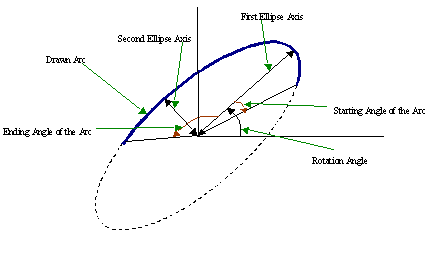
\includegraphics[width=0.5\textwidth]{pics/ellipse.png}

\cvfunc{ellipse2Poly}\label{ellipse2Poly}
Approximates an elliptic arc with a polyline

\begin{lstlisting}
void ellipse2Poly( Point center, Size axes, int angle,
                   int startAngle, int endAngle, int delta,
                   vector<Point>& pts );
\end{lstlisting}
\begin{description}
\cvarg{center}{Center of the arc}
\cvarg{axes}{Half-sizes of the arc. See \cross{ellipse}}
\cvarg{angle}{Rotation angle of the ellipse in degrees. See \cross{ellipse}}
\cvarg{startAngle}{Starting angle of the elliptic arc in degrees}
\cvarg{endAngle}{Ending angle of the elliptic arc in degrees}
\cvarg{delta}{Angle between the subsequent polyline vertices. It defines the approximation accuracy.}
\cvarg{pts}{The output vector of polyline vertices}
\end{description}

The function \texttt{ellipse2Poly} computes the vertices of a polyline that approximates the specified elliptic arc. It is used by \cross{ellipse}.

\cvfunc{fillConvexPoly}\label{fillConvexPoly}
Fills a convex polygon.

\begin{lstlisting}
void fillConvexPoly(Mat& img, const Point* pts, int npts,
                    const Scalar& color, int lineType=8,
                    int shift=0);
\end{lstlisting}
\begin{description}
\cvarg{img}{Image}
\cvarg{pts}{The polygon vertices}
\cvarg{npts}{The number of polygon vertices}
\cvarg{color}{Polygon color}
\cvarg{lineType}{Type of the polygon boundaries, see \cross{line} description}
\cvarg{shift}{The number of fractional bits in the vertex coordinates}
\end{description}

The function \texttt{fillConvexPoly} draws a filled convex polygon.
This function is much faster than the function \texttt{fillPoly}
and can fill not only convex polygons but any monotonic polygon without self-intersections,
i.e., a polygon whose contour intersects every horizontal line (scan
line) twice at the most (though, its top-most and/or the bottom edge could be horizontal).

\cvfunc{fillPoly}\label{fillPoly}
Fills the area bounded by one or more polygons

\begin{lstlisting}
void fillPoly(Mat& img, const Point** pts, const int* npts, int ncontours,
              const Scalar& color, int lineType=8, int shift=0,
              Point offset=Point() );
\end{lstlisting}
\begin{description}
\cvarg{img}{Image}
\cvarg{pts}{Array of polygons, each represented as an array of points}
\cvarg{npts}{The array of polygon vertex counters}
\cvarg{ncontours}{The number of contours that bind the filled region}
\cvarg{color}{Polygon color}
\cvarg{lineType}{Type of the polygon boundaries, see \cross{line} description}
\cvarg{shift}{The number of fractional bits in the vertex coordinates}
\end{description}

The function \texttt{fillPoly} fills an area bounded by several
polygonal contours. The function can fills complex areas, for example,
areas with holes, contours with self-intersections (some of thier parts), and so forth.

\cvfunc{getTextSize}\label{getTextSize}
Calculates the width and height of a text string.

\begin{lstlisting}
Size getTextSize(const string& text, int fontFace,
                 double fontScale, int thickness,
                 int* baseLine);
\end{lstlisting}
\begin{description}
\cvarg{text}{The input text string}
\cvarg{fontFace}{The font to use; see \cross{putText}}
\cvarg{fontScale}{The font scale; see \cross{putText}}
\cvarg{thickness}{The thickness of lines used to render the text; see \cross{putText}}
\cvarg{baseLine}{The output parameter - y-coordinate of the baseline relative to the bottom-most text point}
\end{description}

The function \texttt{getTextSize} calculates and returns size of the box that contain the specified text.
That is, the following code will render some text, the tight box surrounding it and the baseline:

\begin{lstlisting}
// Use "y" to show that the baseLine is about
string text = "Funny text inside the box";
int fontFace = FONT_HERSHEY_SCRIPT_SIMPLEX;
double fontScale = 2;
int thickness = 3;

Mat img(600, 800, CV_8UC3, Scalar::all(0));

int baseline=0;
Size textSize = getTextSize(text, fontFace,
                            fontScale, thickness, &baseline);
baseline += thickness;

// center the text
Point textOrg((img.cols - textSize.width)/2, (img.rows + textSize.height)/2);

// draw the box
rectangle(img, textOrg + Point(0, baseline), textOrg + Point(textSize.width, -textSize.height),
          Scalar(0,0,255));
// ... and the baseline first
line(img, textOrg + Point(0, thickness), textOrg + Point(textSize.width, thickness),
     Scalar(0, 0, 255));

// then put the text itself
putText(img, text, textOrg, fontFace, fontScale,
        Scalar::all(255), thickness, 8);
\end{lstlisting}
        
        
\cvfunc{line}\label{line}
Draws a line segment connecting two points

\begin{lstlisting}
void line(Mat& img, Point pt1, Point pt2, const Scalar& color,
          int thickness=1, int lineType=8, int shift=0);
\end{lstlisting}
\begin{description}
\cvarg{img}{The image}
\cvarg{pt1}{First point of the line segment}
\cvarg{pt2}{Second point of the line segment}
\cvarg{color}{Line color}
\cvarg{thickness}{Line thickness}
\cvarg{lineType}{Type of the line:
  \begin{description}
  \cvarg{8}{(or omitted) 8-connected line.}
  \cvarg{4}{4-connected line.}
  \cvarg{CV\_AA}{antialiased line.}
  \end{description}}
\cvarg{shift}{Number of fractional bits in the point coordinates}
\end{description}

The function \texttt{line} draws the line segment between
\texttt{pt1} and \texttt{pt2} points in the image. The line is
clipped by the image boundaries. For non-antialiased lines
with integer coordinates the 8-connected or 4-connected Bresenham
algorithm is used. Thick lines are drawn with rounding endings.
Antialiased lines are drawn using Gaussian filtering. To specify
the line color, the user may use the macro
\texttt{CV\_RGB(r, g, b)}.


\cvfunc{LineIterator}\label{LineIterator}
Class for iterating pixels on a raster line

\begin{lstlisting}
class LineIterator
{
public:
    // creates iterators for the line connecting pt1 and pt2
    // the line will be clipped on the image boundaries
    // the line is 8-connected or 4-connected
    // If leftToRight=true, then the iteration is always done
    // from the left-most point to the right most,
    // not to depend on the ordering of pt1 and pt2 parameters
    LineIterator(const Mat& img, Point pt1, Point pt2,
                 int connectivity=8, bool leftToRight=false);
    // returns pointer to the current line pixel
    uchar* operator *();
    // move the iterator to the next pixel
    LineIterator& operator ++();
    LineIterator operator ++(int);

    // internal state of the iterator
    uchar* ptr;
    int err, count;
    int minusDelta, plusDelta;
    int minusStep, plusStep;
};
\end{lstlisting}

The class \texttt{LineIterator} is used to get each pixel of a raster line. It can be treated as versatile implementation of the Bresenham algorithm, where you can stop at each pixel and do some extra processing, for example, grab pixel values along the line, or draw a line with some effect (e.g. with XOR operation).

The number of pixels along the line is store in \texttt{LineIterator::count}.

\begin{lstlisting}
\\ grabs pixels along the line (pt1, pt2) from 8-bit 3-channel image to the buffer
LineIterator it(img, pt1, pt2, 8);
vector<Vec3b> buf(it.count);

for(int i = 0; i < it.count; i++, ++it)
    buf[i] = *(const Vec3b)*it;
\end{lstlisting}


\cvfunc{rectangle}\label{rectangle}
Draws a simple, thick, or filled up-right rectangle.

\begin{lstlisting}
void rectangle(Mat& img, Point pt1, Point pt2,
               const Scalar& color, int thickness=1,
               int lineType=8, int shift=0);
\end{lstlisting}
\begin{description}
\cvarg{img}{Image}
\cvarg{pt1}{One of the rectangle's vertices}
\cvarg{pt2}{Opposite to \texttt{pt1} rectangle vertex}
\cvarg{color}{Rectangle color or brightness (grayscale image)}
\cvarg{thickness}{Thickness of lines that make up the rectangle. Negative values, e.g. \texttt{CV\_FILLED}, mean that the function has to draw a filled rectangle.}
\cvarg{lineType}{Type of the line, see \cross{line} description}
\cvarg{shift}{Number of fractional bits in the point coordinates}
\end{description}

The function \texttt{rectangle} draws a rectangle outline or a filled rectangle, which two opposite corners are \texttt{pt1} and \texttt{pt2}.
               

\cvfunc{polylines}\label{polylines}
Draws several polygonal curves

\begin{lstlisting}
void polylines(Mat& img, const Point** pts, const int* npts, int ncontours, bool isClosed,
               const Scalar& color, int thickness=1, int lineType=8, int shift=0 );
\end{lstlisting}
\begin{description}
\cvarg{img}{The image}
\cvarg{pts}{Array of polygonal curves}
\cvarg{npts}{Array of polygon vertex counters}
\cvarg{ncontours}{The number of curves}
\cvarg{isClosed}{Indicates whether the drawn polylines are closed or not. If they are closed, the function draws the line from the last vertex of each curve to its first vertex}
\cvarg{color}{Polyline color}
\cvarg{thickness}{Thickness of the polyline edges}
\cvarg{lineType}{Type of the line segments, see \cross{line} description}
\cvarg{shift}{The number of fractional bits in the vertex coordinates}
\end{description}

The function \texttt{polylines} draws one or more polygonal curves.

\cvfunc{putText}\label{putText}
Draws a text string

\begin{lstlisting}
void putText( Mat& img, const string& text, Point org,
              int fontFace, double fontScale, Scalar color,
              int thickness=1, int lineType=8,
              bool bottomLeftOrigin=false );
enum
{
 FONT_HERSHEY_SIMPLEX = 0,
 FONT_HERSHEY_PLAIN = 1,
 FONT_HERSHEY_DUPLEX = 2,
 FONT_HERSHEY_COMPLEX = 3,
 FONT_HERSHEY_TRIPLEX = 4,
 FONT_HERSHEY_COMPLEX_SMALL = 5,
 FONT_HERSHEY_SCRIPT_SIMPLEX = 6,
 FONT_HERSHEY_SCRIPT_COMPLEX = 7,
 FONT_ITALIC = 16
};
\end{lstlisting}
\begin{description}
\cvarg{img}{The image}
\cvarg{text}{The text string to be drawn}
\cvarg{org}{The bottom-left corner of the text string in the image}
\cvarg{fontFace}{The font type, one of \texttt{FONT\_HERSHEY\_...}}
\cvarg{fontScale}{The font scale factor that is multiplied by the font-specific base size}
\cvarg{thickness}{Thickness of the lines used to draw the text}
\cvarg{lineType}{The line type; see \texttt{line} for details}
\cvarg{bottomLeftOrigin}{When true, the image data origin is at the bottom-left corner, otherwise it's at the top-left corner}
\end{description}

The function \texttt{putText} draws a text string in the image.
Symbols that can not be rendered using the specified font are
replaced question marks. See \cross{getTextSize} for a text rendering code example.

\subsection{XML/YAML Persistence}

\subsection{Clustering and Search in Multi-Dimensional Spaces}

\cvfunc{kmeans}\label{kmeans}

\begin{lstlisting}
double kmeans( const Mat& samples, int clusterCount, Mat& labels,
               TermCriteria termcrit, int attempts,
               int flags, Mat* centers );
enum { KMEANS_RANDOM_CENTERS=0, KMEANS_PP_CENTERS=2, KMEANS_USE_INITIAL_LABELS=1 };
\end{lstlisting}
\begin{description}
\cvarg{samples}{Floating-point matrix of input samples, one row per sample}
\cvarg{clusterCount}{The number of clusters to split the set by}
\cvarg{labels}{The input/output integer array that will store the cluster indices for every sample}
\cvarg{termcrit}{Specifies maximum number of iterations and/or accuracy (distance the centers can move by between subsequent iterations)}

\cvarg{attempts}{How many times the algorithm is executed using different initial labelings. The algorithm returns the labels that yield the best compactness (see the last function parameter)}
\cvarg{flags}{It can take the following values:
\begin{description}
\cvarg{KMEANS\_RANDOM\_CENTERS}{Random initial centers are selected in each attempt}
\cvarg{KMEANS\_PP\_CENTERS}{Use kmeans++ center initialization by Arthur and Vassilvitskii}
\cvarg{KMEANS\_USE\_INITIAL\_LABELS}{During the first (and possibly the only) attempt, the
function uses the user-supplied labels instaed of computing them from the initial centers. For the second and further attempts, the function will use the random or semi-random centers (use one of \texttt{KMEANS\_*\_CENTERS} flag to specify the exact method)}
\end{description}}
\cvarg{centers}{The output matrix of the cluster centers, one row per each cluster center}
\end{description}

The function \texttt{kmeans} implements a k-means algorithm that finds the
centers of \texttt{clusterCount} clusters and groups the input samples
around the clusters. On output, $\texttt{labels}_i$ contains a cluster index for
the sample stored in the $i^th$ row of the \texttt{samples} matrix.

The function returns the compactness measure, which is computed as
\[
\sum_i \|\texttt{samples}_i - \texttt{centers}_{\texttt{labels}_i}\|^2
\]
after every attempt; the best (minimum) value is chosen and the
corresponding labels and the compactness value are returned by the function.
Basically, the user can use only the core of the function, set the number of
attempts to 1, initialize labels each time using some custom algorithm and pass them with
\newline (\texttt{flags}=\texttt{KMEAN\_USE\_INITIAL\_LABELS}) flag, and then choose the best (most-compact) clustering}

\cvfunc{partition}\label{partition}
Splits an element set into equivalency classes.

\begin{lstlisting}
template<typename _Tp, class _EqPredicate> int
    partition( const vector<_Tp>& vec, vector<int>& labels,
               _EqPredicate predicate=_EqPredicate());
\end{lstlisting}
\begin{description}
\cvarg{vec}{The set of elements stored as a vector}
\cvarg{labels}{The output vector of labels; will contain as many elements as \texttt{vec}. Each label \texttt{labels[i]} is 0-based cluster index of \texttt{vec[i]}}
\cvarg{predicate}{The equivalence predicate (i.e. pointer to a boolean function of two arguments or an instance of the class that has the method \texttt{bool operator()(const \_Tp\& a, const \_Tp\& b)}. The predicate returns true when the elements are certainly if the same class, and false if they may or may not be in the same class}
\end{description}

The generic function \texttt{partition} implements a quadratic algorithm for
splitting a set into one or more equivalancy classes, described in \url{http://en.wikipedia.org/wiki/Disjoint-set_data_structure}. The function
returns the number of equivalency classes.

\subsection{Utility and System Functions and Macros}

\cvfunc{alignPtr}\label{alignPtr}
Aligns pointer to the specified number of bytes

\begin{lstlisting}
template<typename _Tp> _Tp* alignPtr(_Tp* ptr, int n=sizeof(_Tp));
\end{lstlisting}
\begin{description}
\cvarg{ptr}{The aligned pointer}
\cvarg{n}{The alignment size; must be a power of two}
\end{description}

The function returns the aligned pointer of the same type as the input pointer:
\[(\_Tp*)(((size\_t)ptr + n-1) \& -n)\]


\cvfunc{alignSize}\label{alignSize}
Aligns a buffer size to the specified number of bytes

\begin{lstlisting}
size_t alignSize(size_t sz, int n);
\end{lstlisting}
\begin{description}
\cvarg{sz}{The buffer size to align}
\cvarg{n}{The alignment size; must be a power of two}
\end{description}

The function returns the minimum number that is greater or equal to \texttt{sz} and is divisble by \texttt{n}:
\[(sz + n-1) \& -n\]


\cvfunc{allocate}\label{allocate}
Allocates an array of elements

\begin{lstlisting}
template<typename _Tp> _Tp* allocate(size_t n);
\end{lstlisting}
\begin{description}
\cvarg{n}{The number of elements to allocate}
\end{description}

The generic function \texttt{allocate} allocates buffer for the specified number of elements. For each element the default constructor is called.


\cvfunc{allocate}\label{allocate}
Allocates an array of elements

\begin{lstlisting}
template<typename _Tp> void deallocate(_Tp* ptr, size_t n);
\end{lstlisting}
\begin{description}
\cvarg{ptr}{Pointer to the deallocated buffer}
\cvarg{n}{The number of elements in the buffer}
\end{description}

The generic function \texttt{deallocate} deallocates the buffer allocated with \cross{allocate}. The number of elements must match the number passed to \cross{allocate}.

\cvfunc{CV\_Assert}\label{CV Assert}
Checks a condition at runtime.

\begin{lstlisting}
#define CV_Assert( expr ) ...
#define CV_DbgAssert(expr) ...
\end{lstlisting}

\begin{description}
\cvarg{expr}{The checked expression}
\end{description}

The macros \texttt{CV\_Assert} and \texttt{CV\_DbgAssert} evaluate the specified expression and if it is 0, the macros raise an error (see \cross{error}). The macro \texttt{CV\_Assert} checks the condition in both Debug and Release configurations, while \texttt{CV\_DbgAssert} is only retained in the Debug configuration.

\cvfunc{error}\label{error}
Signals an error and raises the exception

\begin{lstlisting}
void error( const Exception& exc );

#define CV_Error( code, msg )
#define CV_Error_( code, args )
\end{lstlisting}
\begin{description}
\cvarg{exc}{The exception to throw}
\cvarg{code}{The error code, normally, a negative value. The list of pre-defined error codes can be found in \texttt{cxerror.h}}
\cvarg{msg}{Text of the error message}
\cvarg{args}{printf-like formatted error message in parantheses}
\end{description}

The function \texttt{error} and the helper macros \texttt{CV\_Error} and \texttt{CV\_Error\_} call the error handler. Currently, the error handler prints the error code (\texttt{exc.code}), the context (\texttt{exc.file}, \texttt{exc.line} and the error message \texttt{exc.err} to the standard error stream \texttt{stderr}. In Debug configuration it then provokes memory access violation, so that the execution stack and all the parameters can be analyzed in debugger. In Release configuration the exception \texttt{exc} is thrown.

The macro \texttt{CV\_Error\_} can be used to construct the error message on-fly to include some dynamic information, for example:

\begin{lstlisting}
// note the extra parentheses around the formatted text message
CV_Error_(CV_StsOutOfRange,
    ("the matrix element (%d,%d)=%g is out of range",
    i, j, mtx.at<float>(i,j)))
\end{lstlisting}


\cvfunc{Exception}\label{Exception}
The exception class passed to error

\begin{lstlisting}
class  Exception
{
public:
    // various constructors and the copy operation
    Exception() { code = 0; line = 0; }
    Exception(int _code, const string& _err,
              const string& _func, const string& _file, int _line);
    Exception(const Exception& exc);
    Exception& operator = (const Exception& exc);

    // the error code
    int code;
    // the error text message
    string err;
    // function name where the error happened
    string func;
    // the source file name where the error happened
    string file;
    // the source file line where the error happened
    int line;
};
\end{lstlisting}

The class \texttt{Exception} encapsulates all or almost all the necessary information about the error happened in the program. The exception is usually constructed and thrown implicitly, via \texttt{CV\_Error} and \texttt{CV\_Error\_} macros, see \cross{error}.


\cvfunc{fastMalloc}\label{fastMalloc}
Allocates aligned memory buffer

\begin{lstlisting}
void* fastMalloc(size_t size);
\end{lstlisting}
\begin{description}
\cvarg{size}{The allocated buffer size}
\end{description}
 
The function \texttt{fastMalloc} allocates buffer of the specified size and returns it. When the buffer is 16 bytes or more, the returned buffer is aligned on 16 bytes.

\cvfunc{fastFree}\label{fastFree}
Deallocates memory buffer

\begin{lstlisting}
void fastFree(void* ptr);
\end{lstlisting}
\begin{description}
\cvarg{ptr}{Pointer to the allocated buffer}
\end{description}

The function \texttt{fastFree} deallocates the buffer, allocated with \cross{fastMalloc}.
If NULL pointer is passed, the function does nothing.

\cvfunc{format}\label{format}
Returns a text string formatted using printf-like expression

\begin{lstlisting}
string format( const char* fmt, ... );
\end{lstlisting}
\begin{description}
\cvarg{fmt}{The printf-compatible formatting specifiers}
\end{description}

The function \texttt{format} acts like \texttt{sprintf}, but forms and returns STL string. It can be used for form the error message in \cross{Exception} constructor.

\cvfunc{getNumThreads}\label{getNumThreads}
Returns the number of threads used by OpenCV

\begin{lstlisting}
int getNumThreads();
\end{lstlisting}

The function returns the number of threads that is used by OpenCV.

See also: \cross{setNumThreads}, \cross{getThreadNum}.


\cvfunc{getThreadNum}\label{getThreadNum}
Returns index of the currently executed thread

\begin{lstlisting}
int getThreadNum();
\end{lstlisting}

The function returns 0-based index of the currently executed thread. The function is only valid inside a parallel OpenMP region. When OpenCV is built without OpenMP support, the function always returns 0.

See also: \cross{setNumThreads}, \cross{getNumThreads}.

\cvfunc{getTickCount}\label{getTickCount}
Returns the number of ticks

\begin{lstlisting}
int64 getTickCount();
\end{lstlisting}

The function returns the number of ticks since the certain event (e.g. when the machine was turned on).
It can be used to initialize \cross{RNG} or to measure a function execution time by reading the tick count before and after the function call. See also the tick frequency.

\cvfunc{getTickFrequency}\label{getTickFrequency}
Returns the number of ticks per second

\begin{lstlisting}
double getTickFrequency();
\end{lstlisting}

The function returns the number of ticks per second.
That is, the following code computes the executing time in seconds.
\begin{lstlisting}
double t = (double)getTickCount();
// do something ...
t = ((double)getTickCount() - t)/getTickFrequency();
\end{lstlisting}

\cvfunc{setNumThreads}\label{setNumThreads}
Sets the number of threads used by OpenCV

\begin{lstlisting}
void setNumThreads(int nthreads);
\end{lstlisting}
\begin{description}
\cvarg{nthreads}{The number of threads used by OpenCV}
\end{description}

The function sets the number of threads used by OpenCV in parallel OpenMP regions. If \texttt{nthreads=0}, the function will use the default number of threads, which is usually equal to the number of the processing cores.

See also: \cross{getNumThreads}, \cross{getThreadNum}
